\documentclass{report}

\usepackage{placeins}
\usepackage{graphicx}
\usepackage{pdfpages}
\usepackage{hyperref}
\usepackage{amssymb}
\usepackage{fancyhdr}
\usepackage{enumitem}
\usepackage{threeparttable}
\usepackage{multicol}
\usepackage[compact]{titlesec}
\usepackage{framed}
\usepackage{quoting}
\usepackage{caption}
\usepackage{xcolor}
\usepackage{minted}
\usepackage{tocloft}
\usepackage[a4paper,
            bindingoffset=0cm,
            left=2.5cm,
            right=2.5cm,
            top=2.5cm,
            bottom=3.5cm,
            footskip=1.5cm]{geometry}

% Header & footer
\pagestyle{fancy}
\fancyhf{}
\renewcommand{\headrulewidth}{0pt}
\fancyfoot[C]{\thepage}

% 2-column bibliography
\makeatletter
\renewenvironment{thebibliography}[1]
     {\begin{multicols}{2}[\chapter*{References}]%
      \small
      \list{\@biblabel{\@arabic\c@enumiv}}%
          {\settowidth\labelwidth{\@biblabel{#1}}%
            \leftmargin\labelwidth
            \advance\leftmargin\labelsep
            \@openbib@code
            \usecounter{enumiv}%
            \let\p@enumiv\@empty
            \renewcommand\theenumiv{\@arabic\c@enumiv}}%
      \sloppy
      \clubpenalty4000
      \@clubpenalty \clubpenalty
      \widowpenalty4000%
      \sfcode`\.\@m}
     {\def\@noitemerr
      {\@latex@warning{Empty `thebibliography' environment}}%
      \endlist\end{multicols}}
\makeatother

% Make links blue
\renewcommand\UrlFont{\color{blue}\rmfamily}

% Structured abstract headings
\newcommand{\absdiv}[1]{
  \par
  \noindent\textbf{#1:}
}

% Research questions list
\newlist{rqlist}{enumerate}{1}
\setlist[rqlist, 1]{
  label=\textbf{RQ\arabic{rqlisti}.},
  leftmargin=2cm,
  rightmargin=1.25cm
}

% Block quote
\definecolor{bg}{RGB}{186, 233, 255}
\colorlet{shadecolor}{bg}
\newenvironment{displayquote}
{\begin{samepage}\begin{shaded*}
  \quoting[leftmargin=0pt, vskip=0pt]
}
{\endquoting
  \end{shaded*}\end{samepage}
}

% Section numbering
\renewcommand\thechapter{\arabic{chapter}}
\renewcommand\thesection{\thechapter.\arabic{section}}
\renewcommand\thesubsection{\thesection.\arabic{subsection}}

\makeatletter
\renewcommand\small{%
   \@setfontsize\small\@ixpt{11}%
   \abovedisplayskip 8.5\p@ \@plus3\p@ \@minus4\p@
   \abovedisplayshortskip \z@ \@plus2\p@
   \belowdisplayshortskip 4\p@ \@plus2\p@ \@minus2\p@
   \def\@listi{\leftmargin\leftmargini
               \parsep 0\p@ \@plus1\p@ \@minus\p@
               \topsep 8\p@ \@plus2\p@ \@minus4\p@
               \itemsep0\p@}%
   \belowdisplayskip \abovedisplayskip
}

\frenchspacing
\widowpenalty=10000
\clubpenalty=10000

\setlength\footnotesep{12\p@}
\setlength\textfloatsep{8mm\@plus 2\p@ \@minus 4\p@}
\setlength\intextsep   {8mm\@plus 2\p@ \@minus 2\p@}

\setcounter{secnumdepth}{2}

% \renewcommand{\cftbeforetoctitleskip}{-0.25in} % position TOC title vertically

\renewcommand\@pnumwidth{2em}
\setcounter{tocdepth}{1}
\setlength{\parskip}{0.55em}
\linespread{1.2}

\def\@dottedtocline#1#2#3#4#5{%
  \ifnum #1>\c@tocdepth \else
    \vskip \z@ \@plus.2\p@
    {\leftskip #2\relax \rightskip \@tocrmarg \advance\rightskip by 0pt plus 2cm
               \parfillskip -\rightskip \pretolerance=10000
     \parindent #2\relax\@afterindenttrue
     \interlinepenalty\@M
     \leavevmode
     \@tempdima #3\relax
     \advance\leftskip \@tempdima \null\nobreak\hskip -\leftskip
     {#4}\nobreak
     \leaders\hbox{$\m@th
        \mkern \@dotsep mu\hbox{.}\mkern \@dotsep
        mu$}\hfill
     \nobreak
     \hb@xt@\@pnumwidth{\hfil\normalfont \normalcolor #5}%
     \par}%
  \fi}
\makeatother


\begin{document}

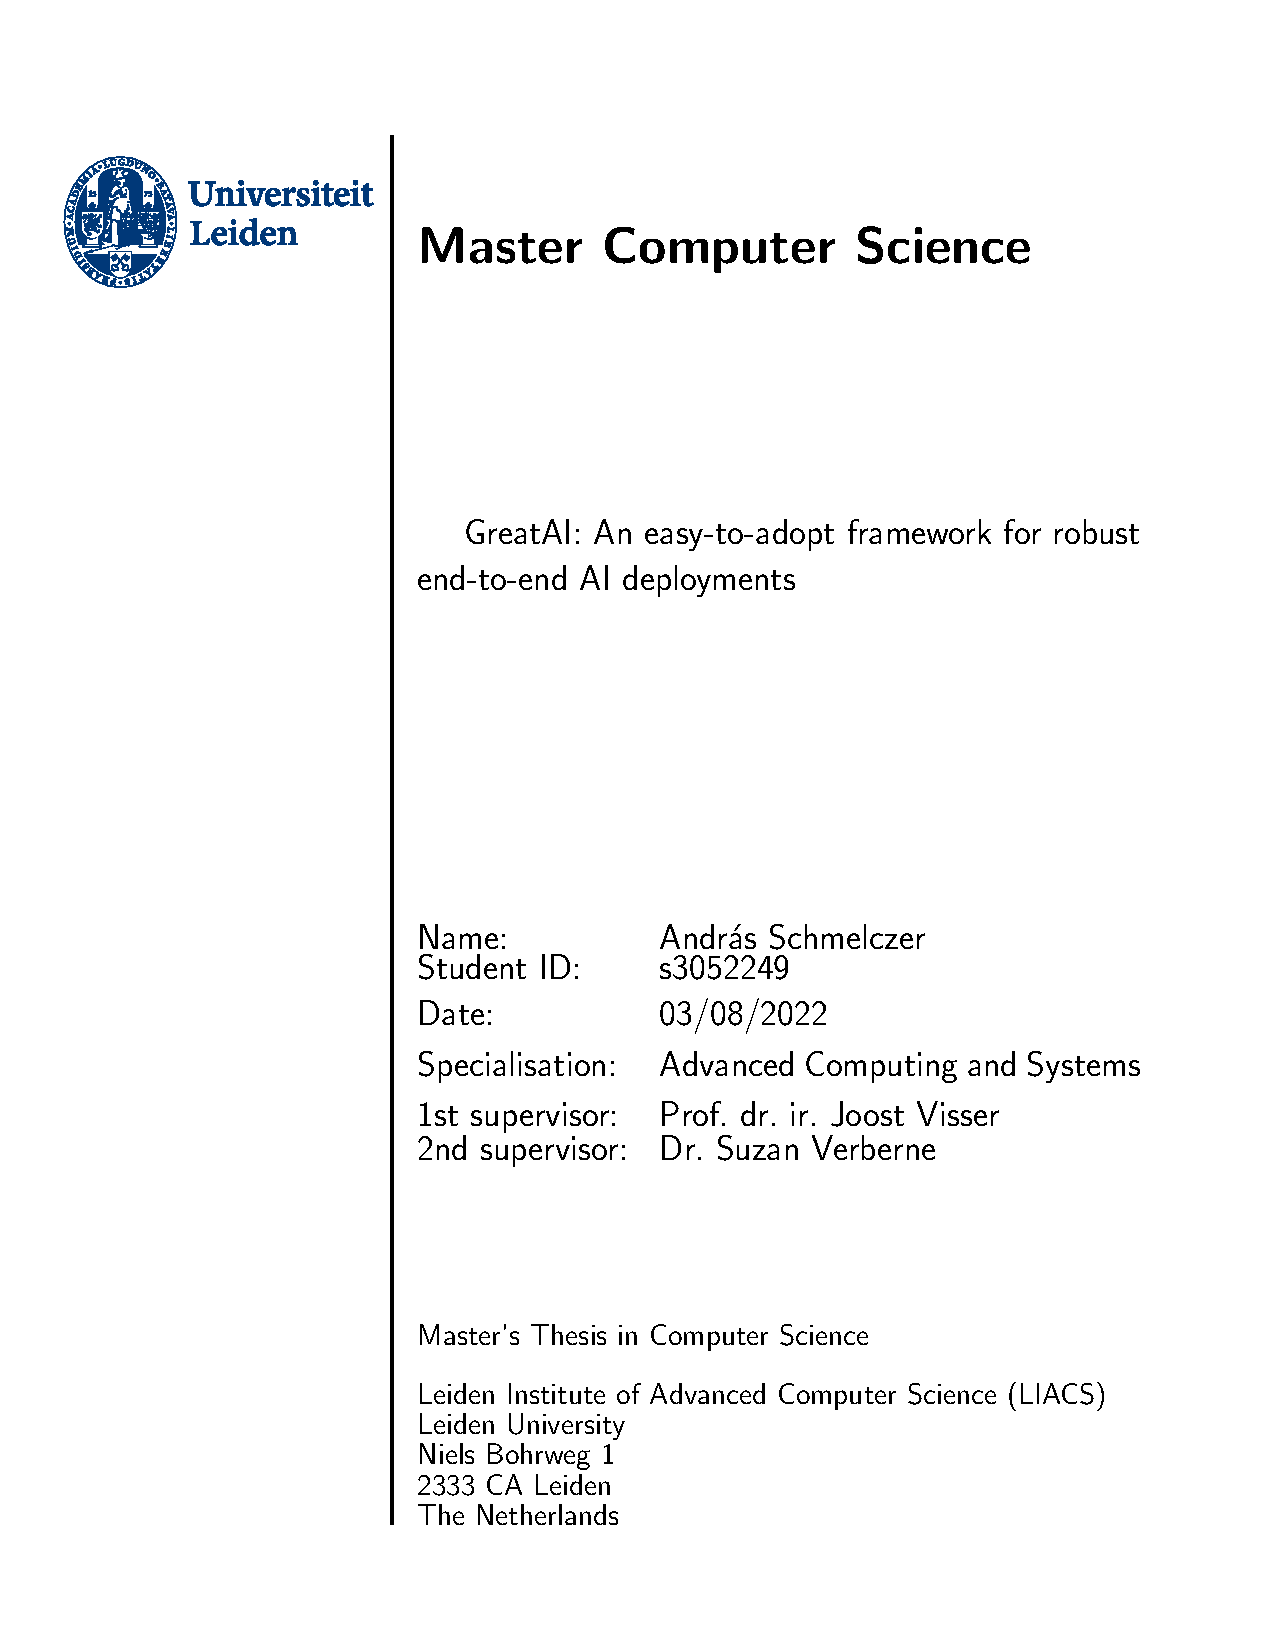
\includepdf[pages=-]{frontpage/frontpage.pdf}
\begin{abstract}

\absdiv{Background}
Despite its long-standing history, artificial intelligence (AI) has only recently started enjoying widespread industry awareness and adoption, partly thanks to the prevalence of libraries that accessibly expose state-of-the-art models. However, the transition from prototypes to production-ready AI applications is still a source of struggle across the industry. Even though professionals already have access to frameworks for deploying AI correctly, case studies and developer surveys have found that many deployments do not follow best practices.

\absdiv{Objective}
This thesis investigates the causes of and a possible resolution to the asymmetry between the adoption of libraries for applying and deploying AI. The potential solution is validated through designing a software framework, called \textit{GreatAI}, which aims to facilitate \underline{G}eneral \underline{R}obust \underline{E}nd-to-end \underline{A}utomated \underline{T}rustworthy deployments while attempting to overcome the practical drawbacks of its predecessors.

\absdiv{Methods}
\textit{GreatAI} serves as a proxy for exploring the proposed design decisions, moreover, its initial focus is limited to the domain of natural language processing (NLP). Its design is validated by applying the principles of design science methodology through iteratively shaping it in two case studies of a commercial NLP pipeline. Subsequently, interviews are conducted with ten practitioners to assess its generalisability.

\absdiv{Results}
\textit{GreatAI} successfully helps implement 33 best practices through an accessible interface. These target the transition between the prototype and production phases of the AI development lifecycle. The feedback from professional data scientists and software engineers showed that ease of use and functionality are equally important in deciding to adopt deployment technologies, and the proposed framework was rated overwhelmingly positively in both dimensions.

\absdiv{Conclusions}
Increasing the overall maturity of industrial AI deployments by devising APIs with ease of adoption in mind is proved to be feasible. Additionally, the created software was deemed effective by experts and a candidate for raising awareness about the utility of following best practices.

\end{abstract}


\tableofcontents

\chapter*{Acknowledgements}
I wish to extend my special thanks to my supervisors, Prof. dr. ir. Joost Visser and Dr. Suzan Verberne, for their invaluable assistance and guidance. I would also like to thank ScoutinScience B.V. for our fruitful collaboration and for allowing me to use their software for experimentation, validation, and demonstration purposes. Last but not least, I would like to individually thank Name, Name, ..., and Name for participating and providing insightful feedback in our interviews.

\chapter{Introduction}

Artificial intelligence (AI) techniques have recently started enjoying widespread industry awareness and adoption; the use of AI is increasingly prevalent in all sectors \cite{wirtz2019artificial,bosch2021engineering}. The reasons behind this are manifold \cite{jordan2015machine}, to name a few: recent breakthroughs in deep-learning, increased public awareness, abundance of available data, access to powerful low-cost commodity hardware, education, but most interestingly, the rise of high-level libraries making ready-to-use state-of-the-art (SOTA) models easily available. The latter practically abolishes the barrier of entry for applying AI --- and with that --- can help use-cases in many areas. 

However, the successful integration of AI components into production-ready applications demands strong engineering methods in order to achieve robust deployments \cite{serban2020adoption}. That is why it is as important as ever to also focus on the quality and robustness of deployed models and software. For instance, the lack of a proper overview of the data transformation steps may lead to suboptimal performance and to introducing unintended biases which may contribute to the ever-increasing negative externality of misused AI \cite{o2016weapons}.

Concerningly, a peculiar tendency seems to be unfolding: even though industry professionals already have access to numerous frameworks for deploying AI correctly and responsibly, case studies and developer surveys have found that a considerable fraction of deployments do not follow best practices \cite{serban2020adoption,haakman2021ai,amershi2019software,de2019understanding,sculley2015hidden}. Utilising state-of-the-art machine-learning (ML) models has become reasonably simple; applying them properly is as difficult and nuanced as ever. 

This thesis sets out to investigate the reasons behind the apparent asymmetry between the adoption of accessible AI libraries and existing reusable solutions for robust AI deployments. It is hypothesised that the primary reason for the underwhelming adoption rate of best practices is the short supply of professionals equally proficient in the domains of both data science and software engineering. Nevertheless, even without their presence, practitioners could rely on frameworks for automated mature deployment processes. However, the barrier of entry for using such existing libraries is too high, especially when compared with the complexity of AI-libraries.

Therefore, a software framework --- called \textit{GreatAI}\footnote{\href{https://github.com/schmelczer/great-ai}{github.com/schmelczer/great-ai}} --- is designed and its design is presented in this thesis. The principal motivation behind the construction of \textit{GreatAI} is to facilitate the responsible and robust deployment of algorithms and models by designing an accessible API in an attempt to overcome the practical drawbacks of other, similar frameworks. Its name stands for its main aim: to assist easily creating \underline{G}eneral \underline{R}obust \underline{E}nd-to-end \underline{A}utomated, and \underline{T}rustworthy AI deployments.

The utility of \textit{GreatAI} is validated using the principles of design science methodology \cite{wieringa2014design} through iteratively designing its API and implementation in a case study concerning the text mining pipeline for a commercial product in collaboration with ScoutinScience B.V.\footnote{\href{https://scoutinscience.com/}{scoutinscience.com}} The goal of the aforementioned software suite is to evaluate technical transfer opportunities in scientific publications. Subsequently, interviews are conducted with practitioners for validating the generalisability of the design.

\section{Research questions}

I hypothesise that facilitating the adoption of AI deployment best practices is viable by finding less complex framework designs which are easier to adopt in order to decrease the negative externality of misused AI. This paper is set out to investigate this hypothesis by answering the following research questions. 

\begin{rqlist}
  \item To what extent does the complexity of AI deployment hinder industrial applications?
  \item What API design techniques can be effectively applied in order to decrease the complexity of correctly deploying AI services?
  \item To what extent can \textit{GreatAI} automatically implement AI deployment best practices?
  \item How adequate is the design of \textit{GreatAI} for helping to apply best practices in other contexts?
\end{rqlist}

In this case, complexity refers to the difficulty faced by professionals (data scientists and software engineers alike) when integrating libraries with their solutions. This could also be described as the barrier of entry or steepness of the learning curve. If the aforementioned hypothesis is correct, the adoption of best practices can be efficiently increased by decreasing this complexity.

AI deployment best practices entail the technical steps that ought to be taken in order to achieve robust, end-to-end, automated, and trustworthy deployments. These are detailed in Section \ref{section:requirements}.

The existence question regarding the problem itself (\textbf{RQ1}) is answered by reviewing the literature of the more than 30 published case studies. \textbf{RQ2} and \textbf{RQ3} are closely connected, the design and evaluation phases utilised to answer them follow an iterative process. They are examined in Chapter \ref{chapter:design} and Chapter \ref{chapter:case} respectively. The final evaluation step is to ascertain the capability of the framework design to generalise beyond a single subdomain and problem context. This question, \textbf{RQ4}, is investigated through interviews with industry professionals in Chapter \ref{chapter:interviews}.

\section{Structure}

The rest of the thesis is organised as follows: Chapter \ref{chapter:background} approaches the problem and the state-of-the-art from three perspectives: the trends of AI library API designs, the experiences gained from practical applications, and a comparison of existing deployment options. Next, the methodology utilised for the subsequent chapters is described in Chapter \ref{chapter:methods}. The design cycle is broken into two chapters, Chapter  \ref{chapter:design} and \ref{chapter:case}. The former clarifies the scope and describes the design principles, while the latter details the specifics of the practical case study, the framework's interaction with it, and technological contributions of the novel design. The results are further validated by conducting interviews with industry professionals in Chapter \ref{chapter:interviews}. The thesis is concluded in Chapter \ref{chapter:conclusion}.

\chapter{Background} \label{chapter:background}

Despite the long-standing history of artificial intelligence (AI), industry awareness and adoption has only recently started to meaningfully catch up \cite{wirtz2019artificial}. At the same time, more regulations and guidelines are being published, for instance, the Ethics guidelines for trustworthy AI by the European Commission's High-Level Expert Group on AI\footnote{\href{https://digital-strategy.ec.europa.eu/en/library/ethics-guidelines-trustworthy-ai}{digital-strategy.ec.europa.eu/en/library/ethics-guidelines-trustworthy-ai}}. This contains seven key requirements, including human agency and oversight, technical robustness, safety, transparency, and accountability. When it comes to accountability, there are meaningful advances being made \cite{raji2020closing}, however, in the case of the other requirements, the situation is more nuanced. Thankfully, the domain of software engineering for machine learning (SE4ML)\footnote{Both in practice and in the literature, this is sometimes also referred to as \textit{AI engineering} and has a large intersection with --- or arguably is the same as --- \textit{MLOps}.} has been working towards finding ways to assist data scientists in ensuring these (and more) expectations are met by their software.

In the following, the context of the problem is presented from three perspectives. Starting with its possible cause: the democratisation of state-of-the-art AI algorithms and models. Subsequently, the challenges encountered when applying AI in practice is outlined by case studies and survey data. Lastly, the existing approaches and solutions are introduced.

\section{Accessible AI} \label{section:accessible-ai}

Most companies prefer not to develop new models but instead reuse prior ones \cite{bosch2021engineering} and they are able to do so increasingly easier. In recent years, there has been a proliferation of highly accessible AI libraries. For example, let us consider the domain of natural language processing (NLP). There are various options for finding AI solutions that work out of the box: FLAIR \cite{akbik2019flair} and Huggingface's transformers \cite{wolf2019huggingface} let developers access the state-of-the-art models and methods in only a couple of lines of code (in many cases 2 or 3). Using transfer-learning, Huggingface enables developers to leverage vast amounts of knowledge learned by pretrained models (such as BERT \cite{devlin2018bert} and its many improved variations) and fine-tune them for their specific use case. The API exposing this is also extremely accessible.

It is not just these two packages, the list of readily available tools is vast: SpaCy \cite{srinivasa2018natural}, Gensim \cite{vrehuuvrek2011gensim}, and scikit-learn \cite{pedregosa2011scikit}, XGBoost \cite{Chen_2016} are other great examples. The situation is similar in all subdomains of artificial intelligence: some domain expertise is --- admittedly --- beneficial but not a hard-requirement. This, combined with the exponentially increasing computing power affordably available to consumers and business alike \cite{sun2019summarizing}, results in AI that is accessible by many.

\section{State of the industry} \label{section:industry}

In contrast with this trend, the software landscape around packaging, deploying, and maintaining machine learning (ML) --- and in general --- data-heavy applications paints a different picture. Fortunately, the related issues and their ramifications have been already thoroughly investigated.

When looking at ML\footnote{The terms AI and ML are often not differentiated and are used as synonyms in practice. For instance, see this study by the FDA \cite{food2019proposed}. ML is a well-defined subdomain of AI, however, most modern AI applications are also ML applications, hence, conflating the two terms may be slightly imprecise but usually not wrong.} code in practice through the lens of technical debt, Sculley et al. \cite{sculley2015hidden} emphasise the repercussions of writing \textit{glue code} between the algorithms and different systems or libraries and define it as an anti-pattern. The consequence of this is the advice against using generic libraries because their rigid API-s may inhibit improvements, cause lock-in, and result in large amounts of glue code. This is a recurring theme in discussions with industry professionals.

Haakman et al. \cite{haakman2021ai} interviewed 17 people at ING which is a well-known fintech company undergoing a digital transformation to embrace AI. They found that the existing tools for ML do not meet the particularities of the field. For instance, a Feature Engineer working in the Data \& Analytics department explained that regular spreadsheets are preferred over existing solutions like MLFlow for keeping track of experiment results. The reason behind this is simplicity. Additionally, multiple other interviewees described the need to self-develop (or highly-customize) dashboards for monitoring deployed models which results in many non-reusable solutions across the company for the same problem. The authors conclude that there is a research gap between the ever-improving SOTA techniques and the challenges of developing real-world ML systems. In short, additional tool support is needed for facilitating the ML lifecycle.

In a case study at Microsoft, Amershi et al. \cite{amershi2019software} interviewed 14 people and surveyed another 551 AI and ML professionals from the company. One of the main concerns surfaced was relating to automation which is a vital cross-cutting concern, especially for testing. At the same time, a human-in-the-loop is still favoured. The survey data pointed out the difficulty posed by integrating AI, especially in the case of less experienced respondents. This was elaborated on by describing the preferences of software engineers as striving for elegant, abstract, modular, and simple systems; in contrast, data tends to be of large volume, context-specific and heterogeneous. Reconciling these inherent differences requires significant effort, nevertheless, Microsoft manages to overcome this with highly sophisticated internal infrastructure.

Using AI is not unique to large companies, in a study conducted with the collaboration of three startups \cite{de2019understanding}, the aim was to fill in the gap of understanding how professionals develop ML systems in small companies. Overall, the results showed they have similar priorities to that of large companies, including an emphasis on the online monitoring of deployed models. However, less structure is present in the development lifecycle, as one interviewee had explained: some steps are left out from time to time because they are forgotten about.

Similarly, Thiée \cite{thiee2021systematic} describes the slow but ever-growing rate of ML adoption by small and medium-sized enterprises (SMEs). With the caveat that many more of these companies would wish to adopt data-driven approaches but are facing new challenges stemming from the domain's complexity.

Serban et al. \cite{serban2020adoption,serban2021practices} describe the results of their global surveys aiming to ascertain the SOTA in how teams develop, deploy, and maintain ML systems. In \cite{serban2020adoption}, they compiled a set of 29 actionable best practices. These were analysed and validated with a survey of 313 participants to discover the adoption rate and relative importance of each best practice. For example, they determined the most important best practice to be \textit{logging production prediction traces}, however, the adoption was measured to be below 40\%. In more than three quarters of the cases, newcomers to AI reported that they \textit{partially} or \textit{not at all} follow best practices. This tendency decreases with more years of experience, reaching a maximum adoption rate of just above 60\%. In a similar fashion, Serban et al. in \cite{serban2021practices}, identify another 14 best practices that concern trustworthy AI mainly through data governance. They strive to complement high-level checklists with actionable best practices. Analysing 42 survey responses reveals a familiar pattern. Most best practices have less than 50\% adoption.

Finally, Bosch et al. \cite{bosch2021engineering} organise and structure the problem space of AI engineering research based on their 16 primary case studies. The authors note the increasing and broad adoption of ML in the industry, while also emphasising that \textit{transition from prototype to production-quality deployment} proves to be challenging for many companies. Large amounts of software engineering expertise is required to create additional facilities for the application such as data pipelines, monitoring, and logging. They define \textit{deployment \& compliance} to be one of the four main categories of problems and describe it as highly underestimated and the source of ample struggle.

\section{Existing solutions} \label{section:existing}

From the previous section, it is noticeable that given enough resources and at the scale of 4195 AI professionals, Microsoft managed to create a comprehensive in-house solution. A similar impression is given by Uber \cite{li2017scaling}; they built a highly sophisticated infrastructure using techniques from distributed and high-performance computing. Though, the authors note that even this solution has its shortcomings in the form rigidity (number of supported libraries and model types) but it still allows the easy extension of the system.

Given the nature of problems faced and amount of available resources, it is not surprising the both of these high-tech, Fortune 500 companies needed to, and did overcome the problems presented by deploying AI. We can learn from their approaches, nonetheless, using them may be infeasible for individuals and SMEs, thus, the issues remain for the majority of practitioners. Luckily, the open-source scene of AI/ML/DS tools, libraries, frameworks, and platforms is thriving. Additionally, there is a considerable number of closed-source --- usually platforms-as-a-service (PaaS) --- solutions next to them. Let us look at some prominent examples.

IBM's AutoAI \cite{wang2020autoai} promises to provide automation for the entire machine learning lifecycle, including deployment. It is a closed-sourced, paid service which --- from their documentation --- seems to focus mostly on non-technical users by providing them with a UI for authoring models. The restrictions caused by the encapsulation of the entire process can be severe. The challenges of integration were emphasised above \cite{sculley2015hidden}. Additionally, an engineer working on Microsoft's comparable solution, the Azure ML Studio, highlighted that once users gain enough understanding of ML, such visual tools can get in their way, and they may need to seek out other solutions \cite{amershi2019software}. Unfortunately, the main value proposition of Azure ML Studio is also to provide a UI for laypeople, and it has also been set to be retired by 2024. Its successor is Azure Machine Learning which shares many similarities with AWS's SageMaker suite \cite{joshi2020amazon}.

SageMaker offers the most comprehensive suite of tools and service; most importantly it has a set of features called \textit{AWS SageMaker MLOps}. This provides easy and/or default implementations for industry best practices described by Serban et al. \cite{serban2020adoption,serban2021practices}. Among others, it promotes the use of CI/CD, model monitoring, tracing, model versioning, storing both data and models on shared infrastructure, numerous collaboration tools, etc. Nonetheless, SageMaker does not enjoy universal adoption as indicated by the survey data. The cause of this may be the lack of self-hosting option and its relatively high prices: many companies prefer on-premise hosting for privacy and financial reasons \cite{bosch2021engineering}. Additionally, vendor lock-in, and possibly --- in the case where it is not already used for the project --- the initial effort required for setting up AWS integration could be possible deterrents.

When it comes to open-source libraries, we can find the MLOps libraries of both TensorFlow and PyTorch: TensorFlow Extended (TFX) \cite{baylor2017tfx} and TorchX\footnote{\href{https://pytorch.org/torchx/latest/}{pytorch.org/torchx/latest}}. TFX comes with a more mature set of features with the caveat that initial time-investment is needed for their setup. The features of TorchX only concern the distributed deployment to a wide range of providers, including Kubernetes (K8s), AWS Batch, or Ray \cite{moritz2018ray}. There is no augmentation for the SE4ML best practices. Given the tight coupling between these libraries and their corresponding ML frameworks, they cannot generalise to models\footnote{The Open Neural Network Exchange (\href{https://onnx.ai/}{onnx.ai}) format could be an option for overcoming these incompatibilities, however, a more universal support is needed for seamless integration.} or algorithms of other frameworks and technologies. 

Open-source platforms also exist such as MLflow and Seldon Core. They both rely on Kubernetes to provide their features. MLflow puts more emphasis on the training phase (in deployment, it lacks a feedback loop which is essential for reaching many of the best-practices), while Seldon Core focuses on the deployment stage. The latter comes integrated with a powerful explanation engine, Alibi Explain \cite{klaise2021alibi}. It also boasts the most comprehensive suite of features including outlier detection, online model selection (with multi-armed bandit theory), and distributed tracing. In short, it seems to be the ideal candidate for the title of \textit{framework for robust end-to-end AI deployments}. Its only downside is the amount of complexity propagated to its clients: it is built on top of Kubernetes, and relies on Helm, Ambasador/Istio, Prometheus, and Jaeger for its features. Hence, the first step in using it is setting up a K8s cluster with all the required components, then when it comes to model deployment, a Kubernetes configuration file has to be created to make use of Seldon's Custom Resource Definition. These are smaller obstacles if the project is already built on top of K8s; however, even then, software engineers with strong cloud and DevOps background are actively required for using Seldon Core.

Additionally, increasing attention is given to ML deployments in embedded systems both from a theoretical \cite{john2020ai} and practical \cite{prado2020bonseyes} point of view. Prado et al. \cite{prado2020bonseyes} survey the available deployment frameworks and end-to-end solutions including those for embedded devices. They note their inefficiencies that come from the lack of features and too much rigidity. They introduce their framework for embedded AI deployments which can be used out-of-the box but also lets the users easily replace and extend its pipeline with steps to fit their changing needs and advancements of the field. While Meenu et al. \cite{john2020ai} present and compare different architectural choices for large-scale deployments in edge-computing. They also note that: \textit{"...there is a need to consider and adapt well established SE practices which have been ignored or had a very narrow focus in ML literature"}.

\begin{table}
\centering
\begin{threeparttable}
\caption{High-level comparison of popular AI deployment platforms and libraries.}
\label{table:platform-comparison}
\setlength{\tabcolsep}{0.25em} % for the horizontal padding
{\renewcommand{\arraystretch}{1.2} % for the vertical padding
\begin{tabular}{|l|c|c|c|c|c|c|c|}
\hline
                             &  AutoAI    & Azure ML   & SageMaker  & TFX        & TorchX     & MLflow     & Seldon Core \\ \hline
Open-source\textsuperscript{1}&            &            &            & \checkmark & \checkmark & \checkmark & \checkmark  \\ \hline
Self-hosted\textsuperscript{1}&            &            &            & \checkmark & \checkmark & \checkmark & \checkmark  \\ \hline
Vendor-agnostic\textsuperscript{2}&            &            &            & \checkmark & \checkmark & \checkmark & \checkmark  \\ \hline
AI-agnostic\textsuperscript{2}&            & \checkmark & \checkmark &            &            & \checkmark & \checkmark  \\ \hline
E2E feedback\textsuperscript{3}&            & \checkmark & \checkmark &            &            &            & \checkmark  \\ \hline
Distributed monitoring\textsuperscript{3}&            & \checkmark & \checkmark & \checkmark & \checkmark & \checkmark\textsuperscript{*} & \checkmark  \\ \hline
Online model selection\textsuperscript{3}& \checkmark\textsuperscript{*} & \checkmark & \checkmark &            &            &            & \checkmark  \\ \hline
Versioning\textsuperscript{3}& \checkmark & \checkmark & \checkmark & \checkmark & \checkmark & \checkmark & \checkmark  \\ \hline
Quick setup\textsuperscript{4}& \checkmark & \checkmark &            &            &            &            &             \\ \hline
No DevOps dependencies\textsuperscript{4}&            &            &            &            & \checkmark &            &             \\ \hline
\end{tabular}}
\begin{tablenotes}
\item[1] For privacy and accountability reasons. \cite{bosch2021engineering}
\item[2] Minimising required glue code. \cite{sculley2015hidden}
\item[3] Implementing best-practices. \cite{serban2020adoption,serban2021practices}
\item[4] Easy integration into existing processes. \cite{haakman2021ai,thiee2021systematic}
\item[*] Only partial support.
\end{tablenotes}
\end{threeparttable}
\end{table}

In summary, the problems expressed in Section \ref{section:industry} can be understood when looking at the available solutions. Table \ref{table:platform-comparison} shows a high-level comparison of frameworks along the dimensions in which practitioners reportedly face difficulties in the \textit{Deployment} stage of the CRISP-DM model \cite{wirth2000crisp}.

\section{Summary}

The surveys and case studies have shown the industry's continuous struggle to evolve their prototypes into robust and responsible production-ready deployments. Simultaneously, platforms aiming to help overcome this challenge already exist but lack widespread adoption. The frequently recurring explanations for not adopting existing solutions surfaced in Section \ref{section:industry} revolve around their complexity and rigidity. These complaints are validated when looking at the available frameworks in Section \ref{section:existing}. While using AI has become more accessible than ever, deploying remains challenging owing to the lack of any \textit{easy-to-use framework for robust end-to-end AI deployments}.

The coexistence of multiple major obstacles along with their promised solutions and the lack of their wide-spread adoption leads us to believe that current frameworks are inadequate for many contexts. There is an unmet need for accessible AI deployment methods. The revolution brought by FLAIR, HuggingFace, and similar libraries for the domain of ML remains unmatched in the domain of AI Engineering.

\chapter{Methods} \label{chapter:methods}

The chosen methodology for this study is Design Science which emphasises the need to design and investigate artifacts in their context \cite{wieringa2014design}. It consists of a design and an empirical cycle. The purpose of the former is to improve a problem context with a new or redesigned artifact. While in the latter, the problem is investigated and its potential treatment is validated concurrently. The design cycle shares similarities with Action Research \cite{davison2004principles}, where the researchers attempt to solve a real-world problem while simultaneously studying the experience of solving said problem. 

As for the empirical cycle, the pragmatist approach is taken since the value of this research lies in its utility. Moreover, pragmatism adopts an engineering approach to research \cite{shull2007guide} which is inline with the philosophy of design science. Additionally, as no research method is without flaws, it is imperative to try to compensate their weaknesses by applying multiple methods. Hence, the study also relies on interviews with professionals for validating the design decisions of \textit{GreatAI}.

\section{Design \& empirical cycles}

The problem context is the difficulty in responsibly transitioning (while following best practices) from prototype industrial AI applications to production-ready deployments. With the possible treatment being libraries with high-level API-s and a set of default settings. It is important to note that \textit{GreatAI} is merely a proof-of-concept, and its aim is to serve as the proxy for the design decisions behind it. Through this, the design can be indirectly evaluated. Hopefully, a by-product will be a library that can be effectively applied to this problem context.

The practical cases used for the evaluation are further elaborated in Chapter \ref{chapter:case}. In short, they focus on individual components of a growing commercial platform\footnote{\href{https://dashboard.scoutinscience.com/}{dashboard.scoutinscience.com}} with the aim of finding tech-transfer opportunities in academic publications. The main input of the system as a whole are PDF-files while the output is a list of metrics describing various aspects of each paper, such as interesting sentences, scientific domains, and the scientific contribution. The output also includes a predicted score used for ranking. This ranking is subsequently processed by the business developers of Technology Transfer Offices (TTO-s) of multiple Dutch and German universities who later give feedback on the results.

Overall, this problem context carries the properties of typical industry use-cases: it utilises a wide-range of natural language processing methods, contains complex interactions between the services, benefits from the integration of end-to-end feedback, and has to provide the clients with a platform that they can rely on in their organisation's core processes. Since the final ranking affects real people, explainability and robustness are also central questions.

The aim of \textit{GreatAI} can be summarised using the terminology of design science in the following way: 
\textit{Facilitate the easy adoption of AI deployment best practices
by finding a less complex framework design 
which is easier to adopt
in order to decrease the negative externality of misused AI.}

However, before generalising, the design of the framework is iteratively refined using the feedback acquired from applying it in practical contexts which in this case is the research and development of a smaller and a more complex AI component using the work-in-progress framework. The treatment is finding a simple design (less cognitively straining to use) which still leads to high-quality deployments as defined in Section \ref{section:requirements}. Questions \textbf{RQ2} and \textbf{RQ3} capture this process; for investigating the feedback acquired from iteratively working on the case --- which is the definition of action research --- is of immense valuable. 

\section{Applicability \& generalisability}

In order to conclusively answer \textbf{RQ3} and \textbf{RQ4}, interviews are conducted from a population of software engineers and data scientists with varying levels of professional background. Since me and my colleagues are likely to have a bias for (or against) the proposed design, the first step of checking its applicability in other practical contexts is to ask the opinion of non-affiliated practitioners.

First, before their interview, interviewees are requested to complete a questionnaire about their last completed AI project; the questions come from a subset of the SE4ML survey. They are also advised to take a quick look at the tutorial page\footnote{\href{https://great-ai.scoutinscience.com/tutorial/}{great-ai.scoutinscience.com/tutorial}} of the documentation. The interviews are divided into two halves. In the first part, after a brief introduction, participants are asked to solve a real-world task by finishing a partially completed example application using GreatAI, they are also encouraged to think out loud so that their feedback can be noted. Successfully completing the task creates a system implementing a known number of best-practices. This way, the added value --- in terms of larger number of implemented best-practices --- can be quantitatively analysed by comparing the qualities of the finished implementation with the previously given answers. 

Notes are taken throughout the interviews and subsequently extended using reflective journaling \cite{halcomb2006verbatim} combined with thematic coding. After which, the insights from the interviewed professionals are distilled using the techniques of thematic analysis \cite{fereday2006demonstrating} following the methodologies of \cite{cruz2019catalog} and \cite{haakman2021ai}. These insights can then be combined with the numerical results to explain and elaborate on them. 

The second half consists of a short survey allowing to create the Technology Acceptance Model (TAM) \cite{davis1989perceived} of the problem context. The ultimate goal of the presented library is to help increase the adoption rate of best practices. In order to reach that goal, first, the library itself has to gain adoption. TAM and its numerous variations provide means of measuring users' willingness of adopting new technologies. TAM has been widely applied in literature \cite{marangunic2015technology} and due to its general psychological origins, it proves to be effective in other areas of technology, not just software \cite{riemenschneider2002explaining}. 

The parsimonious version of TAM will be utilised which was measured to have similar predictive power to that of the original TAM while having fewer variables \cite{wu2011user}. Parsimonious TAM observes three interconnected human aspects that influence the actual behaviour (adoption): perceived usefulness, perceived ease of use, and intention to use. Participants are asked 10 questions corresponding to these aspects about their experience using GreatAI. The questionnaire is shown in Appendix \ref{appendix:questions}. The internal consistency of the answers is calculated using Chronbach's Alpha \cite{bland1997statistics} after which the responses are reflected upon.

\chapter{Designing the framework} \label{chapter:design}

Providing users with a high level of abstraction is not unheard of in the context of practical AI/ML platforms. Many software-as-a-service products offer features for hiding the technicalities of machine learning. However --- as we discussed in Section \ref{section:existing} --- these tend to abstract away the details of both data science and AI engineering, overall hindering the development process. The design proposed here aims to tackle and simplify only the deployment-related concepts.

\section{Scope} \label{section:scope}

As highlighted by several case studies in Chapter \ref{chapter:background}, the transition from prototypes to production-ready systems is often named as the source of unexpected struggle. Maybe it is not a coincidence that a significant portion of the SE4ML best practices should be implemented in this phase. Unfortunately, it is easy to gloss over them while tackling the underestimated difficulties of this \textit{transition}. Therefore, the aim of \textit{GreatAI} is to ease this step of the lifecycle. Consequently, its scope is limited to the \textit{transition} step.

There have been attempts that at least partially address this issue; however, as we saw in Chapter \ref{chapter:background}, these have limitations either from the perspective of best practices or stemming from their difficulty in being adopted. The scope has to be well-defined and limited to provide the best chance of providing an easy-to-adopt solution. To understand the API of a library, users first need to understand its aim and surface and have to become familiar with the problems it solves. Thus, limiting the focus solely to the \textit{transition} step seems reasonable. This step is highlighted in Figure \ref{fig:scope}.

\begin{figure}
    \centering
    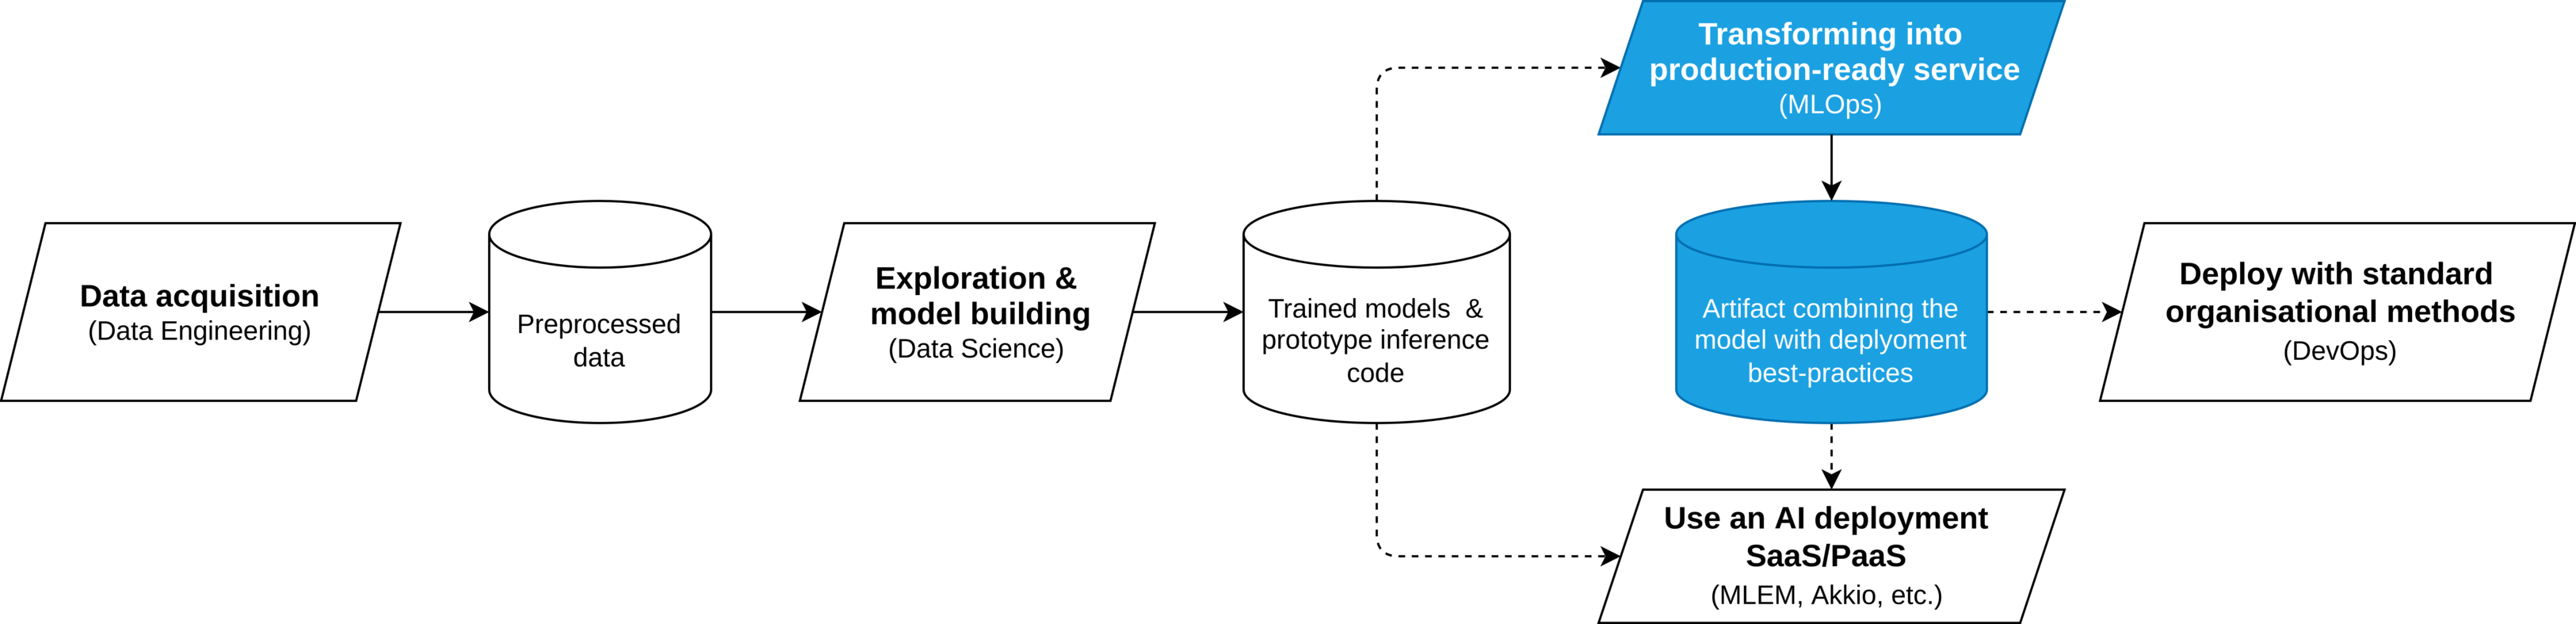
\includegraphics[width=\linewidth]{figures/scope.drawio.png}
    \captionsetup{width=.9\linewidth}
    \caption{Usual process steps (based on \cite{john2020architecting}) in the development lifecycle of a data-heavy software solution. The dashed arrows denote optional paths: after a prototype has been completed, there are multiple options for its deployment. The steps with blue background show the primary scope of \textit{GreatAI}.}
    \label{fig:scope}
\end{figure}

It is interesting to mention that \href{https://xkcd.com/927/}{there is a proliferation} of platform/software as a service (PaaS/SaaS) products for deploying AI\footnote{Such as \href{https://mlem.ai/}{MLEM}, \href{https://streamlit.io/cloud}{Streamlit} or any AutoML SaaS platform, for example, \href{https://www.akkio.com/role/software-engineers}{Akkio} as these often have a one-click deployment feature as well.}. At first, these may look intriguing. However, they tend to only focus on getting code easily deployed in the cloud: AI best practices are not prioritised in this setup. Nevertheless, in many cases, it may be a suitable option to use such a service, and these can also complement \textit{GreatAI} as illustrated in Figure \ref{fig:scope}: first, the prototype is transformed into a \textit{GREAT} service and materialised as a common software artifact implementing best practices. Then, it is either deployed using a deployment SaaS or the organisation's existing software deployment setup.

\section{Requirements} \label{section:requirements}

The best practices (which are referenced throughout the thesis) with which the design is concerned are a subset of those compiled by Serban et al. \cite{serban2020adoption,serban2021practices} and John et al. \cite{john2020architecting}. The core requirements --- set of covered best practices --- for a software solution that has the potential to improve our problem context are presented in the following, along with some explanation and clarification for each of them.

\paragraph{General} Albeit not explicitly in the list of best practices, compatibility is vital in encouraging adoption. Large projects frequently end up depending on numerous packages, each of which may impose some restrictions on the code: since these all have to be satisfied simultaneously, this can result in severe constraints. 

The open-source scene of data-related libraries is vibrant. To take the example of data validation, there are at least four popular choices which offer varying but similar features: \href{https://github.com/SeldonIO/alibi-detect}{Alibi detect}, \href{https://github.com/PAIR-code/facets}{Facets}, \href{https://github.com/great-expectations/great_expectations}{Great Expectations}, and Data Linter \cite{hynes2017data}. The responsibility of choosing the most fitting solution falls on the user. Thus, they should not be limited in this by \textit{GreatAI}. On the contrary, the programming language (PL) of the library may be its only non-general property. Fortunately, the de facto PL for data science is Python, so implementing the library in it should not significantly limit its applicability.

\paragraph{Robustness} In software development, robustness can be achieved by preparing the application to handle errors gracefully, even unexpected ones \cite{bishop1998robust}. Errors can and will happen in practice: storing and investigating what has led to them is required to prevent future ones. In the case of ML, errors might not be as obvious to detect as in more traditional applications (see the above-mentioned data validators). Even if a single feature's value falls outside the expected distribution, unexpected results can happen. In cases where this might lead to real-world repercussions, extra care has to be taken to construct as many safeguards as practicable. \textit{GreatAI} should support its clients in this.

\paragraph{End-to-end} In this case, it refers to end-to-end feedback. That is, feedback should be gathered on the system's real-world performance, which should be taken into account when designing/training the next iteration of the model. Static datasets may fail to capture the changing nature of real life and can become outdated if they are not revised continuously. A well-packaged deployment should make it trivial to integrate new training data.

\paragraph{Automated} The available time of data scientists and software engineers is limited and expensive. For this reason, humans should only be involved when their involvement is necessary. Steps in the development process that can be automated without negative consequences must be automated in order to achieve efficient development processes and let the experts focus on the issues that require their attention the most.

\paragraph{Trustworthy} As detailed in the \href{https://digital-strategy.ec.europa.eu/en/library/ethics-guidelines-trustworthy-ai}{\textit{Ethics guidelines for trustworthy AI}}, human oversight, transparency, and accountability are some of the key requirements for trustworthy AI applications. For increasing public acceptance and trust while minimising negative societal impact, trustworthiness is essential.

The requirements were chosen stemming from their general importance and potential to be mostly implemented by a software framework. That is why these provide an ideal initial direction for tackling the issue. Of course, these do not cover all best practices; for instance, the ones relating to organisational processes fall outside the realm of computer science.

\section{Design principles} \label{section:principles}

Before diving into the concrete issues being solved, let us detail the principles we use while implementing their solutions. As implied in Section \ref{section:scope}, the Unix philosophy \cite{ritchie1978unix,salus1994quarter} of software design is followed. Most notably, the design goal that encourages to \textit{write programs that do one thing and do it well}. Apart from providing a clear and simple picture of the intended use cases for the library, this is also in line with the main notion of \textit{A Philosophy of Software Design} \cite{ousterhout2018philosophy}: APIs should be narrow and deep. 

A narrow width refers to having a small exposed surface area, i.e. having a small number of functions and classes in the public API. In contrast, depth implies that each accomplishes an involved, complex goal. In a way, the width of an API is the price users have to pay (the effort required for learning it) to use it, while the depth is analogous to the return they get from it. Having to learn little and being provided with a lot of functionality maximises return on investment (ROI), hence, developer experience (DX). 

Moreover, the theoretical frameworks presented in \textit{The Programmer's Brain} \cite{hermans2021programmer} provides us with explanations and vocabulary from psychology for arguing about the cognitive aspects of API design. In the following, two of them will be used for detailing the design principles: cognitive dimensions of code bases (CDCB) which is an extension of the cognitive dimensions of notation (CDN) framework \cite{blackwell2001cognitive}, and linguistic anti-patterns \cite{arnaoudova2016linguistic}. The former comes with a set of dimensions describing different (often competing) cognitive aspects of code that influence one's ability to perform specific tasks.

Linguistic anti-patterns provide guidelines for improving consistency and decreasing the false sense of consistency when there is none. Also, choosing the right names for identifiers can help activate information stored in the long-term memory, making it quicker to comprehend and easier to reason about the code \cite{deissenboeck2006concise}. Finding the most accurate and useful names is more challenging than it first seems. Accuracy and usefulness are already often competing goals: the more precise the name, the longer and, therefore, less convenient to use \cite{butler2009relating}. In short, good names are essential to good APIs; consciously considering the implications of names must be an integral part of the design process.

Nonetheless, simple APIs come with a high technical cost. The library has to implement these in a way that still allows for high performance in production \cite{kleppmann2017designing} and avoids being tied to specific libraries or technologies. Inspiration for the latter may be gained from the ML pipelines of Prado et al. \cite{prado2020bonseyes}: they show that more freedom can be achieved with plug-and-play steps and preconfigured defaults. 

\subsection{Default configuration}

Existing frameworks frequently suffer from the entanglement of numerous levels of abstractions.\footnote{\href{https://grugbrain.dev/\#grug-on-apis}{grugbrain.dev/\#grug-on-apis}} Instead of exposing each implementation detail and encouraging users to interact with most of them, these can be abstracted away in a more high-level layer. Even where configuration may be helpful for advanced users, default values can still be chosen automatically while providing an override option where necessary.

For example, tracing the evaluations and the model versions used in a distributed fashion is very much expected of a trustworthy system. Hence, turning this feature on by default but allowing opting-out from it can result in less scaffolding required from the library's users. It also decreases their up-front cognitive load, which by definition flattens the learning-curve \cite{hermans2021programmer}. Similar features can be imagined for providing a service API for the algorithms, giving feedback, marking outliers, and more.

Being \textit{automated} is listed as a requirement, but it is imperative to only automate for simplifying and not for hiding decisions. More precisely, guessing must not be a part of automation. For instance --- an otherwise handy WebGL library --- TWGL.js, has a feature for automatically guessing the type of vectors based on their names. Suppose it matches the \texttt{/colou?r/i} pattern. In that case, it is treated as a vector with three components\footnote{\href{https://github.com/greggman/twgl.js/blob/e3a8d0ed09f7f5cd4be0e4cb5976081c2b5013aa/src/attributes.js\#L139}{\tiny github.com/greggman/twgl.js/blob/e3a8d0ed09f7f5cd4be0e4cb5976081c2b5013aa/src/attributes.js\#L139}}. It is easy to imagine that this can help in certain scenarios. Still, it does so at the cost of immense confusion when correctly renaming a variable breaks the application. In CDCB, this equates to scoring high on the dimension of \textit{Hidden dependencies} and low on \textit{Visibility}.

Learning from this, any guessing must be avoided to create a pleasant API. However, this conflicts with providing defaults for each configuration value. Even if these would be reasonable defaults derived from educated guesses, they are still merely guesses. Nevertheless, if the users were required to specify each configuration option, that would lead to vastly more boilerplate code. This verbosity is captured by the \textit{Diffuseness} dimension of CDCB and, of course, should be minimised.

To resolve this conflict, \textit{GreatAI} should have recommended values instead of defaults. This can mean a context object (as suggested in \cite{ousterhout2018philosophy}), which contains the result of each design consideration that has to be made for a service's deployment. If not configured manually, the recommended values are applied automatically, just like defaults. However, the values chosen for each parameter must be clearly highlighted. Coming from the library's single responsibility, the number of parameters should not be immense; hence, the user can be expected to comprehend them instead of just being overwhelmed and skipping them.

This way, the library attempts to notify its user about the existence of these decisions but does not force them to decide manually. As a result, no initial configuration is needed for starting out with the library (high \textit{Provisionality}, low \textit{Diffuseness}), and the dependencies are not hidden since they are explicitly highlighted.

\subsection{Documentation}

Little value can be derived from software without good documentation; undoubtedly, good documentation is a prerequisite for adoption. Documentations come in many shapes: modern integrated development environments (IDEs) tend to show a popup of a function's description when requested (for instance, on mouse hover), but at the same time, a more comprehensive online manual and example projects are also still expected. Descriptive error messages can also be viewed as documentation.

The library must have quality documentation for all categories. Accordingly, for structuring it, the \textit{Diátaxis} philosophy is preferred \cite{Procida_Diataxis_documentation_framework} which prescribes dividing documentation into 4 parts along 2 axes: practical-theoretical and passive-active consumption. The four quadrants derived from this are tutorials, how-to guides, references, and explanations.

Once again, we might notice two competing interests: the level of detail and the length of the documentation. For example, FastAPI\footnote{\href{https://fastapi.tiangolo.com/async/\#concurrent-burgers}{fastapi.tiangolo.com}}, a popular Python web framework, has extensive descriptions and explanations on all topics related to Python's import system, the HTTP protocol, concurrency, deployment, and more. The actual framework's documentation is sprinkled over these overly broad topics. This is undoubtedly helpful for beginners to acquire knowledge from a single place. Yet, this high level of accessibility actually hinders the process of finding the relevant sections; in CDCB, this shows a trade-off between the support of \textit{Searching} and \textit{Comprehension} tasks. Diátaxis' take is that linking to external resources about the library's domain is welcome, but the documentation must have a single responsibility: describing the library itself.

A large portion of software documentations is automatically generated from source code, and this has the advantage of always keeping it in sync with code changes. However, it might also signal that the API is too large because it is inconvenient for the developers to document it by hand. Striking the right balance between handcrafted and automatically extracted documentation may be a vital component of good documentation.

When it comes to example code, showing at least a minimal starter code and the way of customising it has to be showcased front and centre. It is a well-known observation that developers only read the documentation when they are stuck, and there might be some merit to this. Helping them not get stuck --- by providing a starter code from which they can explore the API using IntelliSense-like solutions --- should be preferred. Take the example of another widely popular Python web framework, Flask\footnote{\href{https://flask.palletsprojects.com/en/2.1.x/}{flask.palletsprojects.com/en/2.1.x}}, at this time, has 324 homogeneously styled links on its landing page. Out of these, only two lead to the quick-start code. Of course, it is not hidden, but we argue that the DX could be improved by displaying where to start more prominently.

\subsection{Developer experience}

Subjectively, a key component of good DX is \textit{Progressive evaluation} through which development can become a highly iterative, experimental process. This is well-understood by popular data science tools, such as Jupyter Notebooks. \textit{GreatAI} also has to support some level of this, for example, in the form of auto-reload on code changes. Further key ingredients of good DX are consistency and discoverability. To give one more example, the MySQL connector's Python implementation\footnote{\href{https://dev.mysql.com/doc/connector-python/en/}{dev.mysql.com/doc/connector-python/en}} has a cursor object which exposes a \texttt{fetchone} method. Even though this naming scheme is not conventional in Python since it does not follow \href{https://peps.python.org/pep-0008/}{PEP 8}, at least the API is intuitive: changing \texttt{sql\_cursor.fetchone()} to \texttt{sql\_cursor.fetchall()} returns all items instead of just one. Using good and consistent names is the key to good DX.

At the same time, Python codebases are rarely strictly object-oriented (OO). They are a mix of the functional, data-driven, and OO paradigms. Consequently, relying on classes for grouping related functions is not always desirable; therefore, it is even more imperative to name similar functions similarly. This helps discoverability and chunking \cite{hermans2021programmer}, which amounts to quicker comprehension.

There is one more reason to prefer consistency: humans have limited short-term memory (STM) \cite{miller1956magical}. Even though flags as function parameters are frowned upon by some \cite{martin2009clean}, they can be useful, especially when configuring libraries. However, if there is no convention for the default value of a flag, clients have to remember the flag's name and initial value simultaneously, quickly overloading their STM. Thus, in the codebase, all defaults must be the same, let us say, \texttt{False}. Sometimes, it can result in a \textit{disable} prefix, which may turn into a double negation. Nevertheless, users should never encounter this since the doubly-negated version is the default; thus, it is only singly negated when overriding it. This approach also implies that something may be recommended to be turned on by default.

\section{Architecture} \label{section:architecture}

Although API design has been the central subject so far, it is worth remembering that APIs are usually expected to have corresponding implementations. \textit{GreatAI} is no exception. As laid out in Section \ref{section:principles}, we strive for narrow and deep interfaces; thus, it is time to address the \textit{depth} component.

\textit{GreatAI} stands on the shoulders of numerous open-source packages and integrates them to provide its various features. The most fundamental dependencies and the entire library in context are shown in Figure \ref{fig:technologies}. Given a Python script or a Jupyter notebook, \textit{GreatAI} transforms the specified prediction functions into a production-ready deployment, deployable either as a Docker image, WSGI-server, or an executable relying on \texttt{uvicorn}. The complete list of dependencies can be found in the repository\footnote{\href{https://github.com/schmelczer/great-ai/blob/main/pyproject.toml}{github.com/schmelczer/great-ai/blob/main/pyproject.toml}}.

\begin{figure}
    \centering
    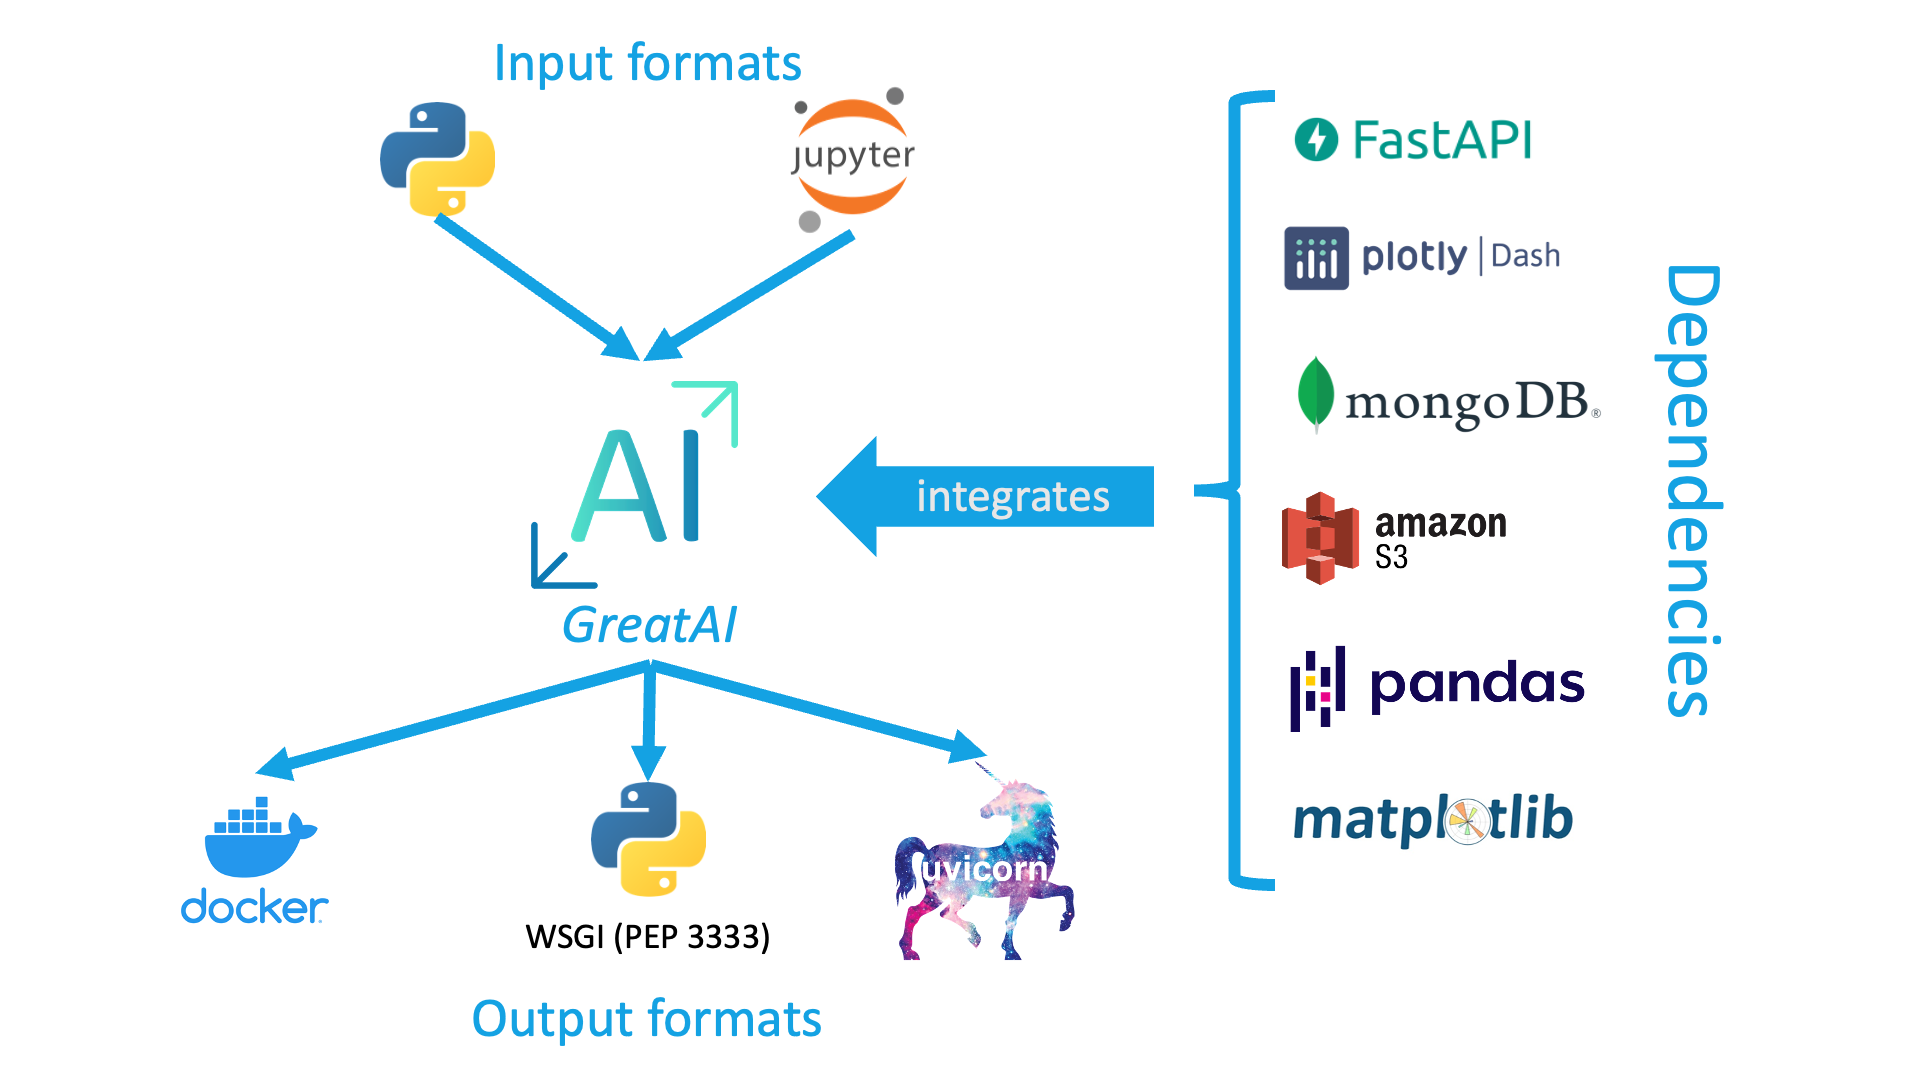
\includegraphics[width=0.65\linewidth]{figures/technologies.png}
    \captionsetup{width=.9\linewidth}
    \caption{A very high-level overview of \texttt{GreatAI} in its context. The main dependencies are also highlighted.}
    \label{fig:technologies}
\end{figure}

The general theme in the implementation is that each explicit best practice should have its distinct, loosely-coupled functions or classes. When collaboration opportunities arise, such as persisting the model versions (\nth{1} component) into prediction traces (\nth{2} component), there are three primary conduits for realising them. These are the \texttt{context} object responsible for the global configuration per process, the \texttt{FunctionMetadataStore} specifying the expected behaviour of each prediction function, and finally the \texttt{TracingContext} that is created anew for each prediction input (session).

After refining the framework with feedback gathered from case studies and users, we will end up with the core architecture presented in Figure \ref{fig:architecture}. The implementation is mixed-paradigm, combining the expressiveness of functional and the design patterns of object-oriented programming (OOP) in order to maintain an overall low complexity. Reflection is also utilised, especially for run-time type-checking and generating the API definitions and dashboard components. Regardless, the architecture is still presented with a syntax similar to the class diagrams of UML2 \cite{Rumbaugh2004} because it provides the freedom to express even the non-OOP design aspects.

For the sake of brevity, Figure \ref{fig:architecture} does not show all fields, and some related entities have been combined, e.g. the \textit{GroundTruthAPI} box represents the \texttt{add\_ground\_truth}, \texttt{query\_ground\_truth}, and \texttt{delete\_ground\_truth} functions. The client project can also access most of the presented entities, but these optional dependency arrows are not shown in the diagram. The \texttt{utilities} submodule is also left unexpanded; almost all of its functions are orthogonal with the exception of \texttt{parallel\_map}. The latter follows a textbook producer-consumer model facilitated by queues and event signals \cite{wang2020producer}.

\begin{figure}
    \centering
    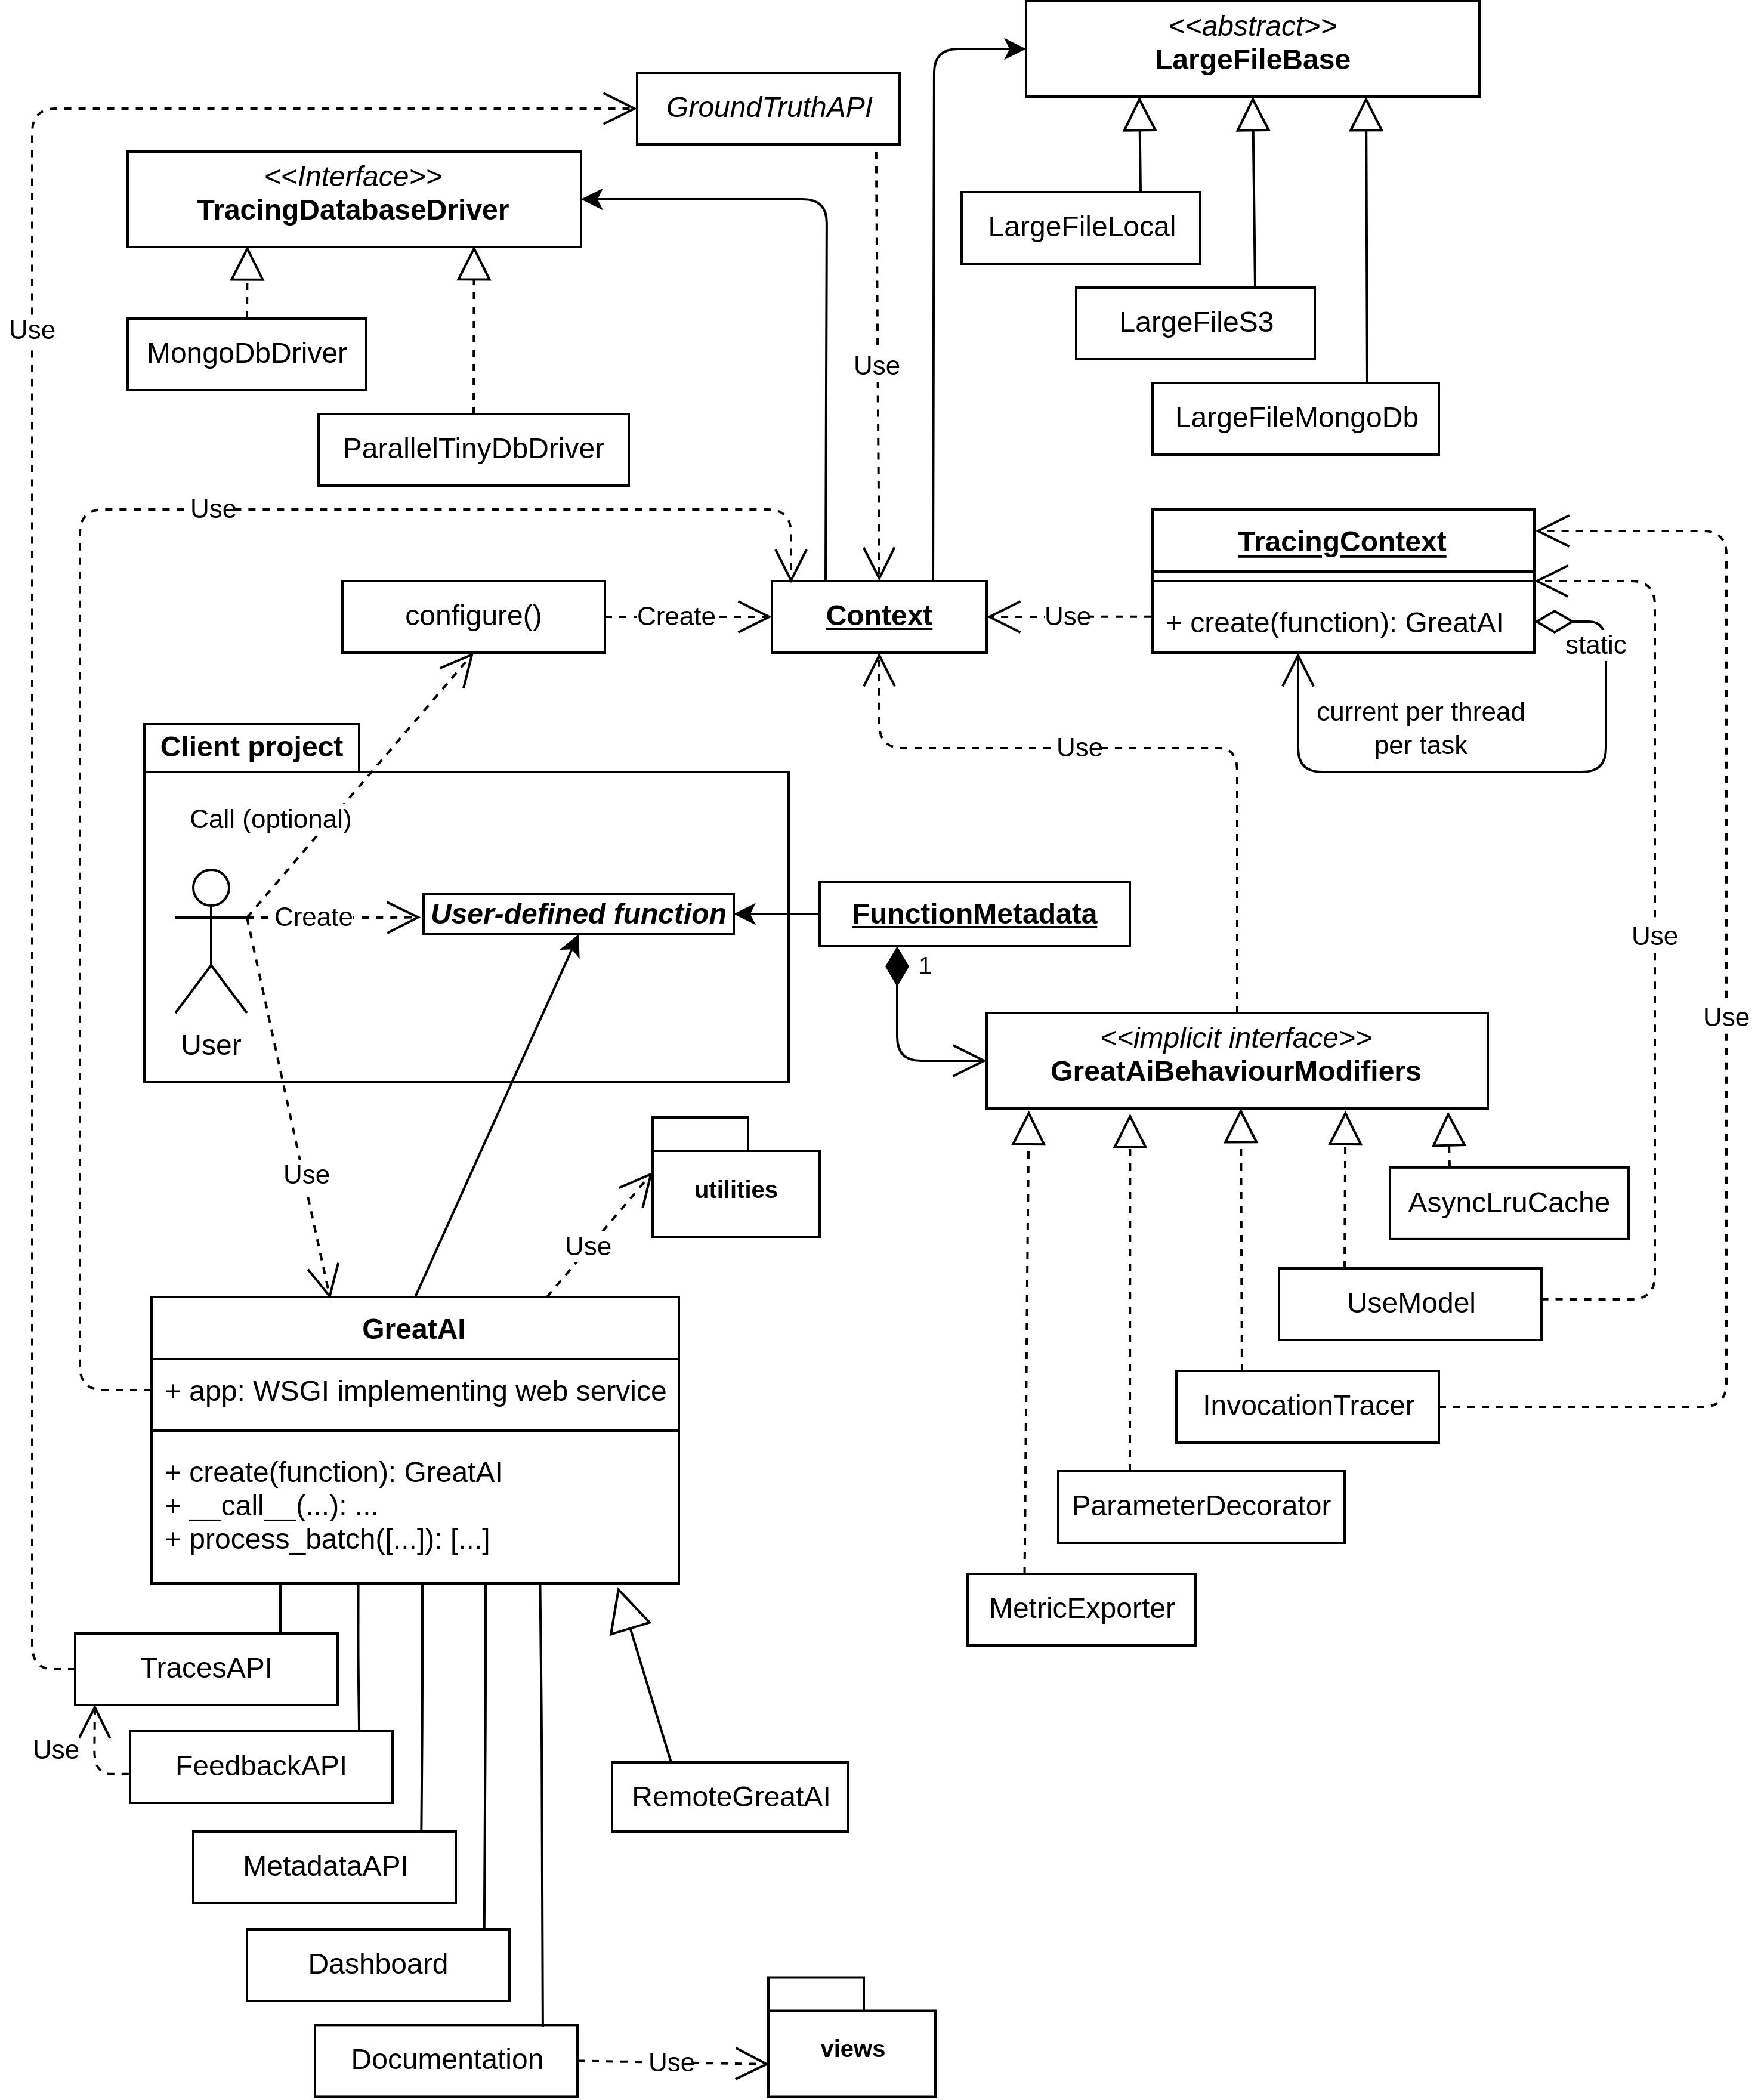
\includegraphics[width=\linewidth]{figures/architecture.png}
    \captionsetup{width=.9\linewidth}
    \caption{The core architecture of \textit{GreatAI} illustrated with syntax loosely-based on UML2 \cite{Rumbaugh2004}. Given its framework nature, the expected client project and the actor integrating it are highlighted; the associations between the framework and the client project are achieved through the use of decorators.}
    \label{fig:architecture}
\end{figure}

\chapter{The ScoutinScience platform} \label{chapter:case}

The core product of \href{https://scoutinscience.com/}{ScoutinScience B.V.} is its platform\footnote{\href{https://dashboard.scoutinscience.com/}{dashboard.scoutinscience.com}}. The clients are technology-transfer offices of Dutch and German universities, government organisations (e.g.: Wetsus), and corporates (e.g.: Heraeus Group, Ruma Rubber B.V.) who wish to extend the scope of their R\&D activities. ScoutinScience connects to multiple data sources of academic publications and integrates them into a single database. Each new publication is evaluated with a suite of AI components that ultimately determine its technology transfer potential. Other features are also extracted that help the users get a quick overview of the authors, topics, and contributions of a given piece of research.

Each client organisation gets to see a different filtered view of this database ranked by the predicted probability of technology transfer opportunities being present. The main motivation is to make these business developers' and other professionals work more efficient by showing them which papers have the highest chance of being considered interesting by them. 

To achieve this, we have a service-based architecture \cite{kleppmann2017designing} on the backend-side --- apart from the data integration, communication, and business logic --- it is made up of services wrapping simpler (phrase-matching, Naïve Bayes) and more sophisticated (conditional random fields, transformer) models. As we will soon see, these can also depend on each other, for instance, based on the predicted scientific domain, a different model can be chosen for scoring certain aspects of papers.

I was among the first engineers on the team which has grown considerably in the past two years. While architecting, designing, and integrating more and better models into our software solution, I experienced the same difficulties as were described in Chapter \ref{chapter:background}. The gap between prototypes and production-ready services is larger than it seems. It is also larger than it should be. This had motivated me to investigate the state-of-the-art and I have found that it is insufficient in many cases. Since the ScoutinScience platform is a quite typical example of applying AI in the industry, it will serve as the real-life case, problem context, and testbed for attempting to design a solution which can hopefully advance the state-of-the-art.

In this chapter, the process of designing \textit{GreatAI} is described along with how it fits into real-life use-cases. First, a simple experiment is presented which leads to the implementation of a software service, subsequently, as the feature-set of the library grows and matures, a more complex component is developed. Lastly, the final version of the design is presented and qualitatively evaluated to verify how well it satisfies the requirements described in Section \ref{section:requirements}.

\section{Domain classification with Naïve Bayes} \label{section:simple-case}

Using different models for slight variations of the same problem is commonplace in the industry. For instance, UberEats has a vast, hierarchical set of models for every country, region, and city for calculating the estimated time of delivery \cite{li2017scaling}. We have also found that in order to best process an academic publication, knowing its domain is essential. The reason for this can be (among others) the wildly different vocabularies of different domains. For example, the term \textit{framework} in computer science almost always refers to a software artifact (usually implying high tech-transfer potential). In contrast, in most other domains, \textit{framework} is used to describe theoretical models that are less central to practical applications. Of course, it is not merely the meaning of the terms but, more importantly, their distribution that varies significantly. Therefore, the topic of this section is to design and develop a domain prediction model for academic papers.

\subsection{Background}

Fortunately, this is one of the oldest text classification tasks. In fact, Maron introduced the Naïve Bayes classifier in 1961 \cite{maron1961automatic} for precisely this purpose: classifying documents' subjects. However, it is still an active problem when it comes to academic texts, as indicated by Elsevier-funded research carried out by Rivest et al. \cite{rivest2021level}. They created a 176-class classification problem for comparing bibliometric and deep-learning approaches. However, this comparison is made difficult because 44\% of the labels are \textit{assigned suboptimally} in the ground-truth dataset.

Prior work evaluated SciBERT \cite{beltagy2019scibert} --- a BERT \cite{devlin2018bert} model pretrained on academic publications --- on a simpler version of the task in which the domains of sentences\footnote{Sentences are more appropriate units for processing due to SciBERT's maximum token length of 512 which comes from its attention mechanism's quadratic complexity \cite{vaswani2017attention}.} have to be decided\footnote{\href{https://paperswithcode.com/sota/sentence-classification-on-paper-field}{paperswithcode.com/sota/sentence-classification-on-paper-field}}. It achieved an F1-score of $0.6571$ after being pretrained on the Semantic Scholar Corpus (SSC) \cite{Lo2020S2ORCTS} and finetuned on the train split of the Microsoft Academic Graph (MAG) dataset \cite{wang2019review}\footnote{SciBERT was applied to a preprocessed version (\href{https://github.com/allenai/scibert/tree/master/data/text_classification/mag}{github.com/allenai/scibert/tree/master/data/text\_classification/mag}) of this dataset.}. To my knowledge, no other published work exists on this sentence classification task. This may be explained by the task's lack of practical relevance and contrived nature (uniform label distribution), as we will see in the following subsection.

\begin{displayquote}
\textbf{Design note} After getting familiar with the context, it is time to focus on experimenting and developing our domain prediction service. At the same time, the difficulties encountered should be noted and integrated into \textit{GreatAI}'s design.
\end{displayquote}

\subsection{Data}

Two datasets will be considered for the experiments. SciBERT's MAG and the SSC. The former is used to compare the results with SciBERT's, while the latter is utilised for training a model for production purposes because it has 19 labels compared with MAG's seven, and it also contains abstracts instead of just sentences; thus, it is more fitting for our practical use-case.

SciBERT's version of the MAG dataset has 84 thousand and 22.3 thousand sentences in its train and test splits, respectively. These are mostly in English and have all punctuation and casing removed. Each sentence is classified as belonging to one of seven fields. Figure \ref{fig:mag-distribtion} shows that the classes have a uniform distribution. 

\begin{figure}
    \centering
    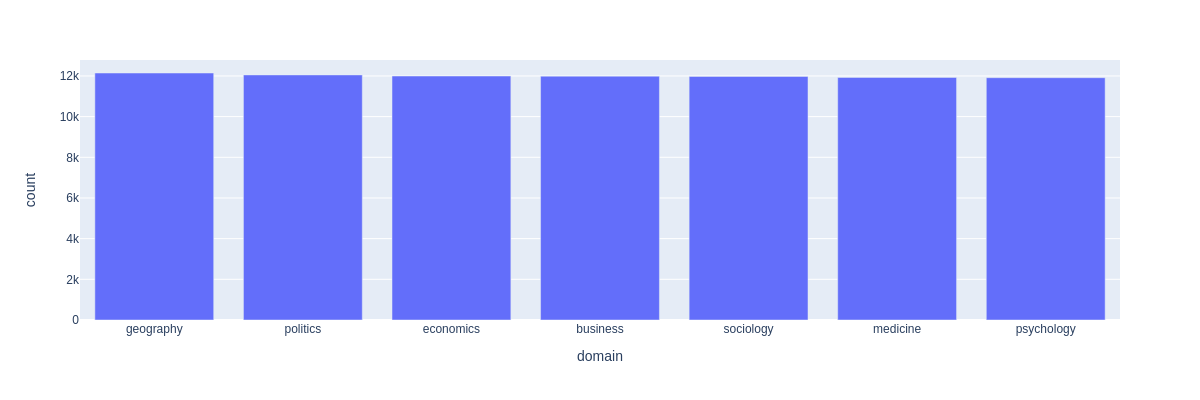
\includegraphics[width=0.5\linewidth]{figures/mag-distribution.png}
    \captionsetup{width=.9\linewidth}
    \caption{Class distribution of the MAG  \cite{wang2019review} dataset's 84000 sentences in its \textit{train} split.}
    \label{fig:mag-distribtion}
\end{figure}

SSC is much larger: it contains over 80 million abstracts. Having more data certainly helps in sampling the term distribution more accurately; nonetheless, the law of diminishing returns applies, especially when using simple models. Therefore, the data will be randomly downsampled to give us a more manageable couple of hundreds of megabytes of abstracts. We can see the distribution of class labels in Figure \ref{fig:ss-distribution}. The dataset is considerably less balanced: \textit{medicine} is by far the most voluminous field.

\begin{figure}
    \centering
    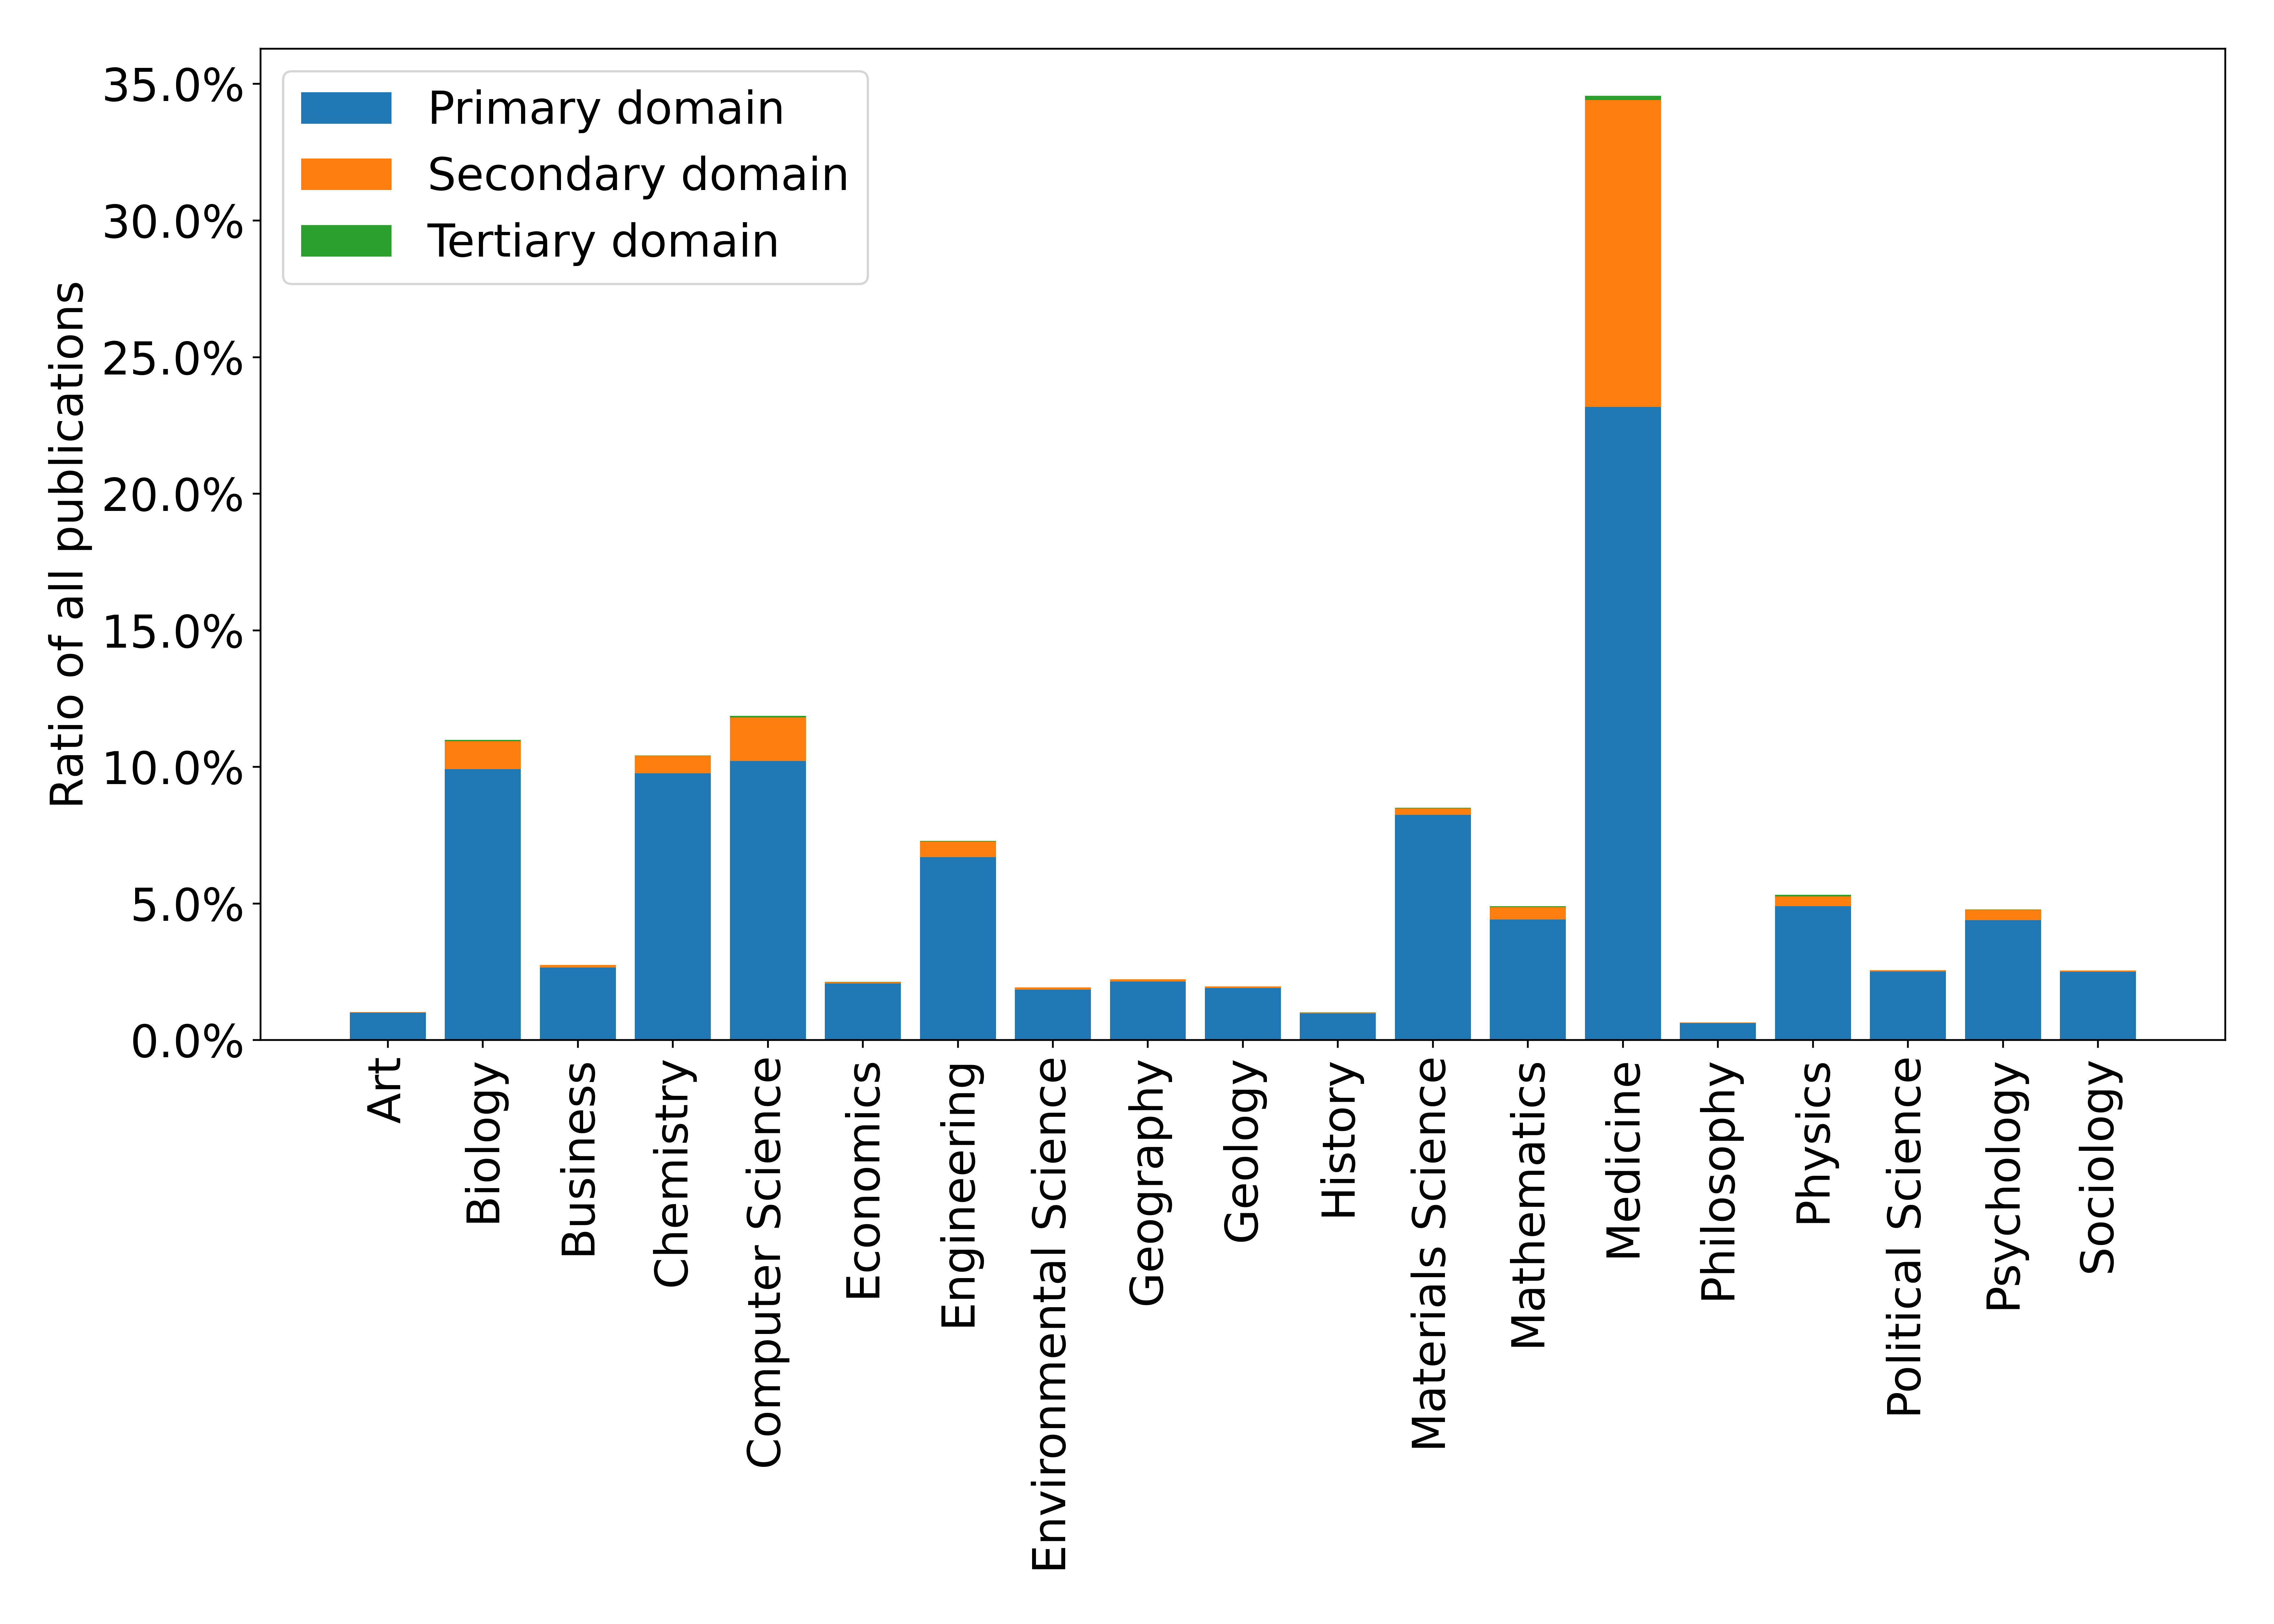
\includegraphics[width=0.8\linewidth]{figures/ss-distribution.png}
    \captionsetup{width=.9\linewidth}
    \caption{Label distribution of the Semantic Scholar dataset \cite{Lo2020S2ORCTS}. Each publication may be assigned at most three domains.}
    \label{fig:ss-distribution}
\end{figure}

\begin{displayquote}
\textbf{Where should we store this data?} ``On my machine'' seems like an easy answer. However, if we have a team working with the data or it has intrinsic value, it must be stored in an easy-to-access, potentially redundant way. Serban et al. \cite{serban2020adoption} expressed this need in the following best practice: \textit{Make Data Sets Available on Shared Infrastructure (private or public)}. Meanwhile, wherever data is stored, it should also be versioned to satisfy the next best practice: \textit{Use Versioning for Data, Model, Configurations, and Training Scripts}.
\end{displayquote}

MAG needs no further preprocessing if we aim to match SciBERT's setup \cite{beltagy2019scibert}. However, since SSC contains heaps of metadata, the relevant parts have to be extracted and preprocessed. In this case, these are the concatenation of the abstract's text and the paper's title along with the paper's domains (there can be multiple domains for a single paper: it is a multi-label classification task). Lastly, the non-English entries are discarded because we only expect to process papers in English.

\begin{displayquote}
\textbf{How should we preprocess the data?} These simple processing steps (filter, map, project) are almost always present in the data science lifecycle. For example, cleaning the input text from various HTML, OCR, PDF, or \LaTeX \hskip 0.12cm extraction artifacts is almost always necessary for text analysis. This is captured in the \href{https://se-ml.github.io/practices}{AI best practices collection} under the following category: \textit{Write Reusable Scripts for Data Cleaning and Merging}. Also, the best practice of \textit{Test all Feature Extraction Code} is somewhat applicable: the applied processing steps must not introduce unwanted artifacts.
\end{displayquote}

\subsection{Methods}

Our aims are twofold: (1) to evaluate a sentence classification model on MAG and compare it with prior art; and (2) to retrain and apply this model for classifying publication metadata (including abstracts). This would allow the ScoutinScience platform to select an appropriate processing pipeline which has been trained on a matching vocabulary (and domain) for each publication. 

It seems reasonable that only considering the distribution (frequencies) of individual terms may be sufficient. For testing this hypothesis, a unigram language model (Multinomial Naïve Bayes) is constructed, and its accuracy is compared with SciBERT's. The former definitely aligns with the advice to \textit{Use The Most Efficient Models}.

Using the MNB implementation of scikit-learn \cite{pedregosa2011scikit}, it only took a couple of lines to create, hyperparameter-optimise, and test a text classifier. Including data loading and visualisations, it takes 71 lines of code (LOC) to be more precise. \footnote{The code is available at \href{https://great-ai.scoutinscience.com/tutorial/}{great-ai.scoutinscience.com/tutorial}.} This further proves how simple it is to use standard packages. The code can be considered for satisfying the \textit{Automate Hyper-Parameter Optimisation} best practice since it also implements an automated hyperparameter sweep. 

The sentences are tokenised into words and vectorised with TF-IDF (with logarithmic term frequency) \cite{buckley1985implementation}, the hyperparameters found via 10-fold cross-validation on the \textit{train} split lead to filtering out tokens which occur in fewer than five documents or more than 5\% of the documents.

\begin{displayquote}
\textbf{What could be automated here?} As discussed in Section \ref{section:accessible-ai}, libraries exposing algorithms and even SOTA models can already be considered mature and accessible. In this case, only scikit-learn was utilised, but subjectively, most popular libraries have a similarly easy-to-use API. Therefore, I see no urgent need for further action regarding the \textit{experimentation} step of the lifecycle in connection with the AI best practices.
\end{displayquote}

\subsection{Results \& Discussion}

\begin{figure}
    \centering
    \includegraphics[width=0.8\linewidth]{figures/mag-confusion.png}
    \captionsetup{width=.9\linewidth}
    \caption{Confusion matrix of a Naïve Bayes classifier on the MAG dataset's sentences. The matrix is normalised column-wise. Notice, how most mistakes happen between semantically similar classes, for instance: \textit{politics} -- \textit{sociology} or \textit{business} -- \textit{economics}.}
    \label{fig:mag-confusion}
\end{figure}

\begin{figure}
    \centering
    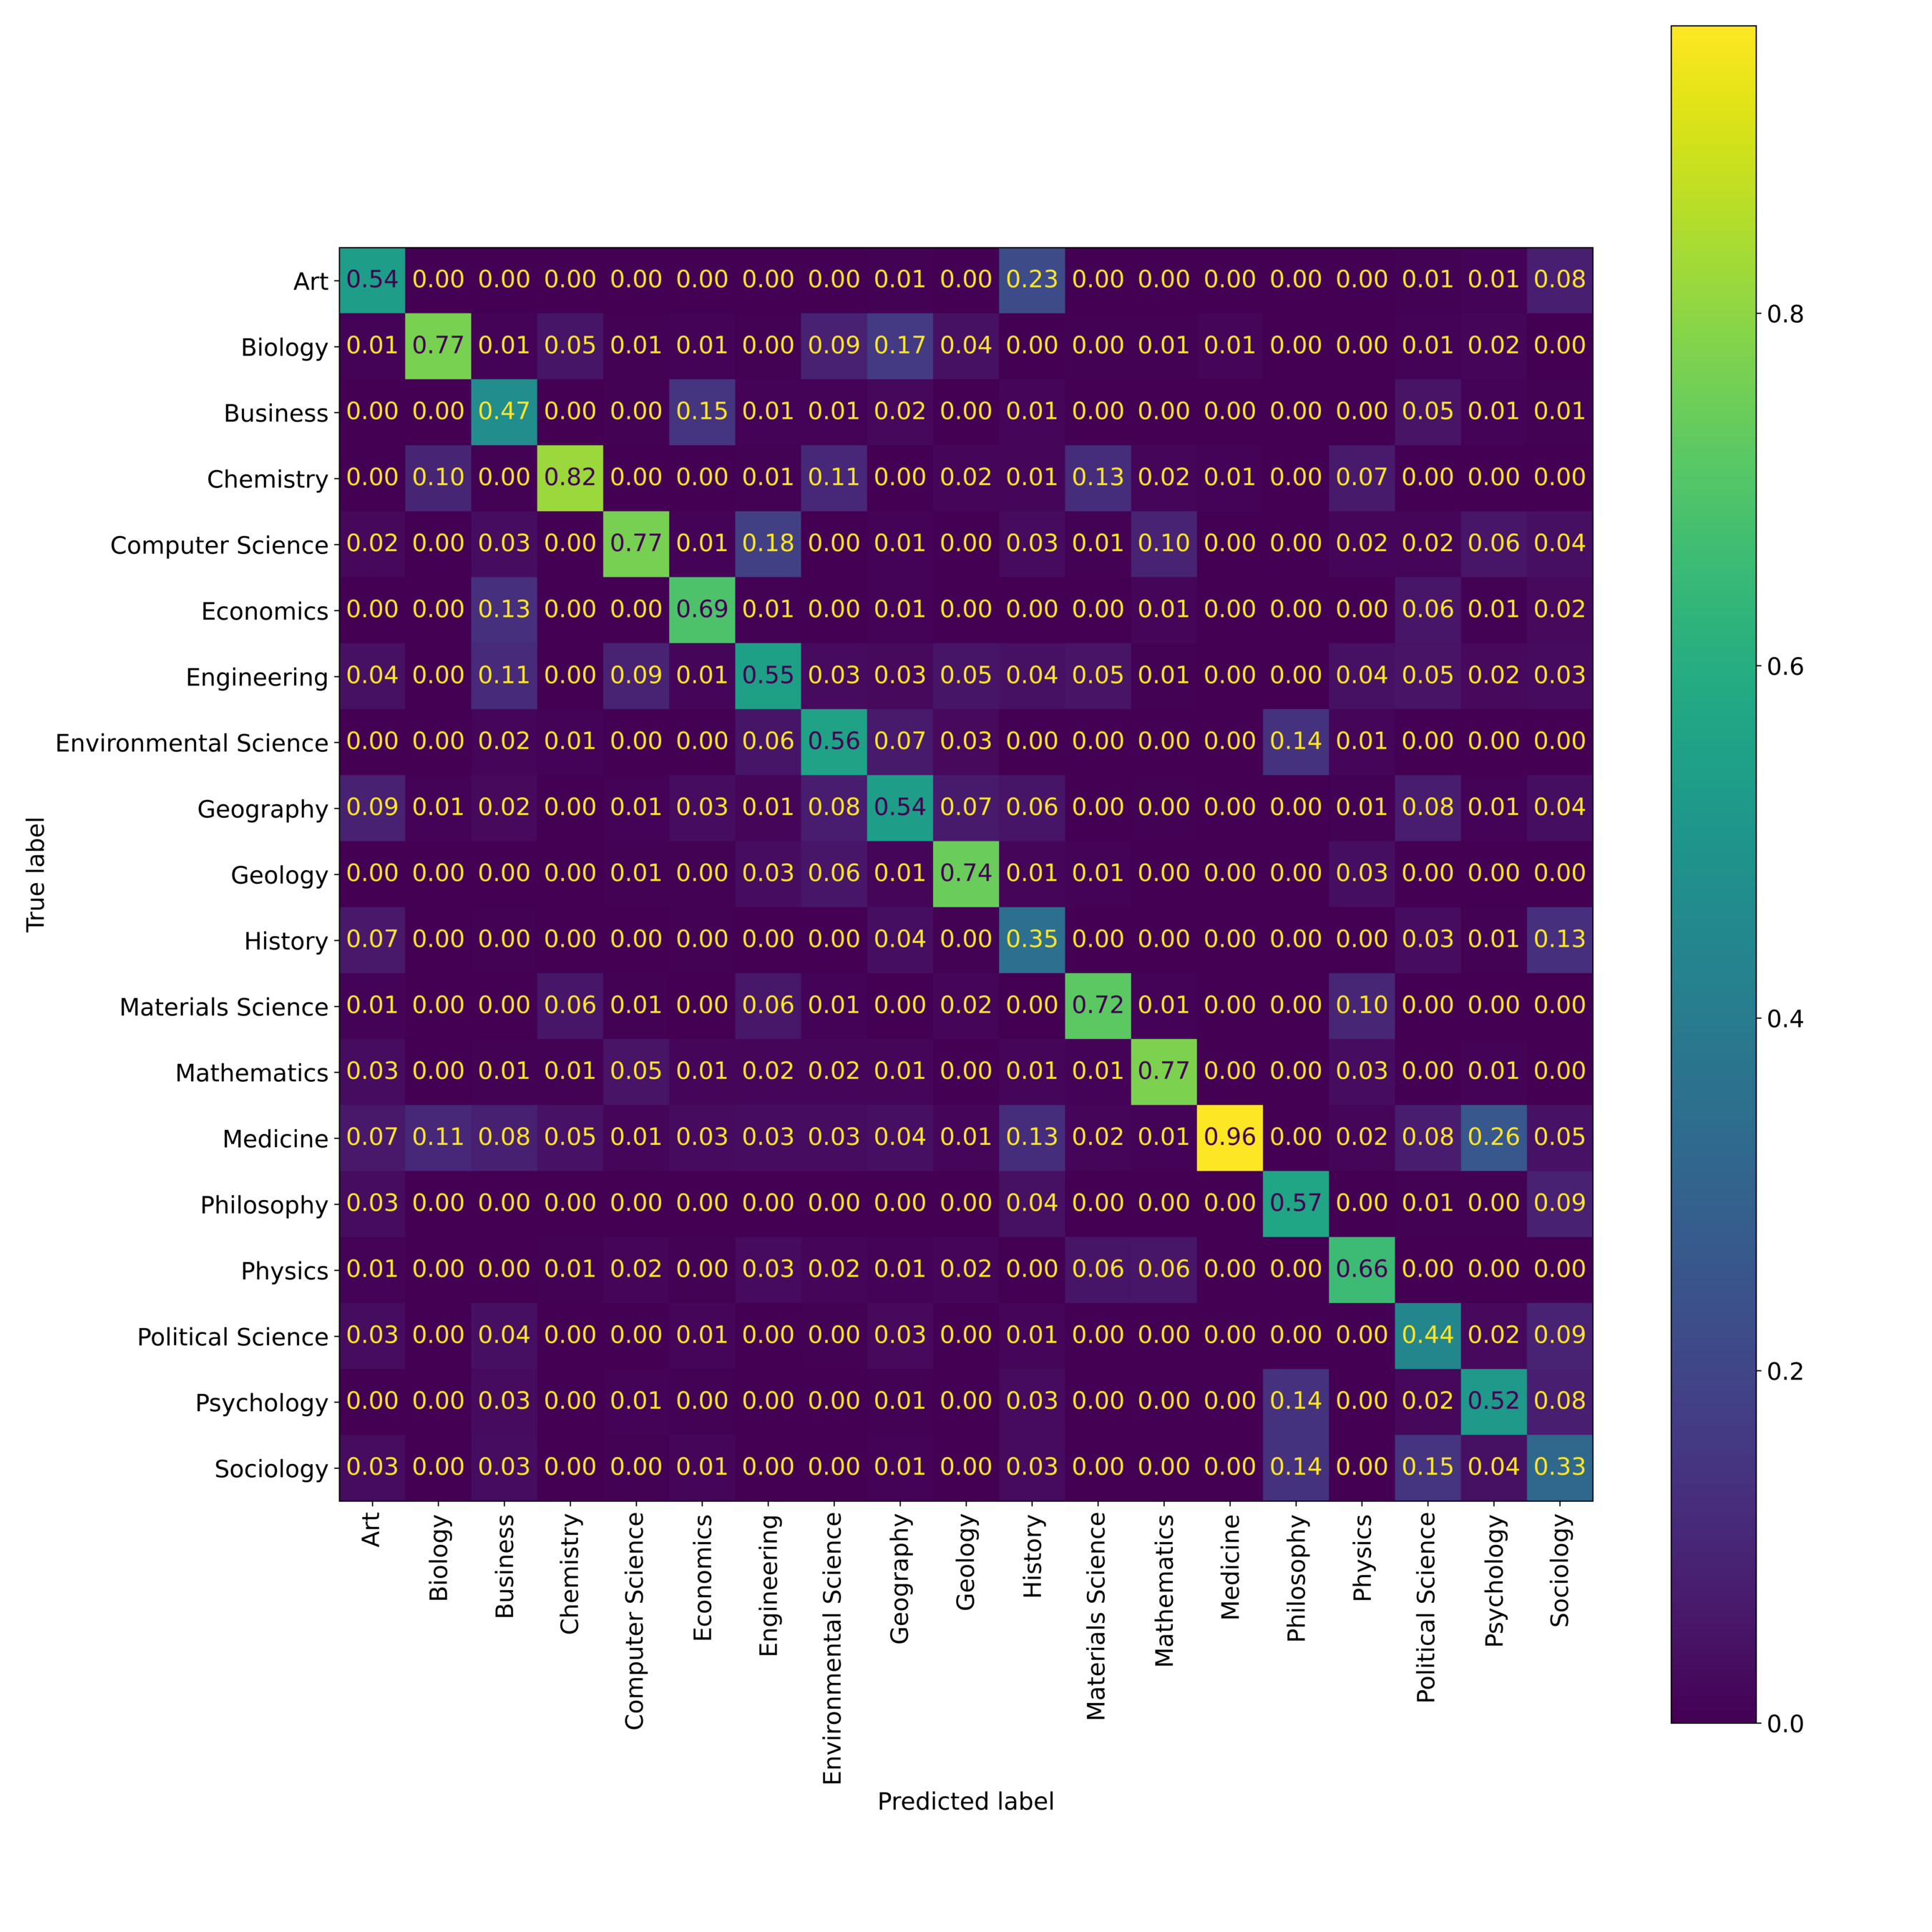
\includegraphics[width=\linewidth]{figures/ss-confusion.png}
    \captionsetup{width=.9\linewidth}
    \caption{Confusion matrix of a Naïve Bayes classifier on the SSC dataset's sentences. The matrix is normalised column-wise. Notice, how most mistakes happen between semantically similar classes, for instance:  \textit{philosohpy} -- \textit{sociology} or \textit{history} -- \textit{art}.}
    \label{fig:ss-confusion}
\end{figure}

When this model is applied to the \textit{test} split of MAG, we get the confusion matrix of Figure \ref{fig:mag-confusion}. This Naïve Bayes classifier achieves a whopping $0.6795$ F1 score. This is $2.3\%$ more than SciBERT's on the same dataset. Thus, it seems that MNB clearly outperforms SciBERT for this particular use case: it is not only more accurate, but its model is magnitudes smaller, while it is also considerably faster to train (or finetune in the case of SciBERT) and use (its running time is in the order of milliseconds per publication). It also has no upper limit on the input length. Thus, this experiment validates choosing MNB for the task over SciBERT.

It is, of course, not entirely surprising that the sophisticated transformer architecture of SciBERT is not necessary for a straightforward task like this. Apart from phrases, the relations between separate words of a sentence do not carry nearly as much discriminative power as the identity of the terms \cite{hand2001idiot}; hence, there is little reason for using an attention mechanism. The fact that SciBERT even works in any way on this task is already a testament to its general applicability. Nevertheless, this short experiment has proved that we can safely opt for using MNB for production.

Since Multinomial Naïve Bayes is best at returning a single label and SSC has multiple labels per datapoint: for evaluation purposes, it is checked whether the returned label is contained in the labels of the ground truth. On this dataset, MNB achieves a lower macro-average F1 score of 0.59.\footnote{The code for this is available at \href{https://great-ai.scoutinscience.com/examples/simple/deploy}{great-ai.scoutinscience.com/examples/simple/deploy}.} The weighted-average F1 is 0.70, and the overall accuracy is also 70\%. The substantial difference between the macro and weighted averages comes from the unbalanced distribution of the labels.

The lower F1 score is not surprising because this dataset has more than twice as many classes. Additionally, the mistakes made are defensible when we look at Figure \ref{fig:ss-confusion}: most of them are between close or related classes.

\begin{displayquote}
This is the usual point where papers conclude: a proof-of-concept/prototype has been built, and its performance demonstrated, measured --- and usually --- explained. Nonetheless, in an industrial setting, our problem is far from being solved: it has yet to be deployed.
\end{displayquote}

\subsection{Deployment}

First, an inference function needs to be written that can take input on the fly and calculate a corresponding prediction. Since we aim to follow the best practices, namely: \textit{Explain Results and Decisions to Users} and \textit{Employ Interpretable Models When Possible}, explaining the results is expected. Fortunately, with our simple model, it is easy to determine the most influential weights, thus, words. The explanations are derived by taking the top 5 tokens from the input text ranked by their feature weights. The last deployment step may be to provide access to our model for others.

\begin{displayquote}
\textbf{How do we provide an interface for the inference function?} We either have an offline or online inference workflow (or both). For the former, we have to provide a way to use it in batch processing; a simple Python function may be adequate for this purpose, though allowing it to be easily (or automatically) parallelised would improve its consumers' DX. If it is an online workflow, we must have a service running continuously and accepting input at any time. This can be achieved by a remote procedure call (RPC) interface or, more commonly, a web API. Developers usually refer to these as REST APIs, and sometimes, they even follow the conventions of REST. Either way, we must develop a wrapper over the service to make it available to other internal/external consumers.
\end{displayquote}

According to the body of research on the adoption of best practices, this is where many real-world projects conclude. This also happens to be \textbf{the gap}. Believing that solely focusing on the research and experiments is good enough is a fallacy: when following this approach, the deployment step ends up being a rushed attempt of wrapping the \textit{AI} and putting it in the production environment. This is, inarguably, a deployment. However, it likely follows very few of the best practices, which can lead to suboptimal real-life performance, lack of accountability, lack of opportunity to improve, and possibly an overall negative societal impact.

\begin{displayquote}
\textbf{How could we implement more best practices?} The most notable missing software/operations features are the lack of automated deployment, automated regression testing, online monitoring, persisting the traces, graceful error-handling, taking feedback on the results (if possible in the use-case), calculating the online accuracy based on the feedback, and retraining the model if necessary using novel data. These all correspond to best practices.
\end{displayquote}

\section{Bridging the gap with GreatAI}

First, let us revisit the library's scope for clarification. As concluded in Section \ref{section:scope}, \textit{GreatAI} should ease the \textit{transition} step between prototypes and production-ready deployments. However, this leaves open the question of what constitutes this step. There are cross-cutting concerns; for example, feature extraction is implemented and used in the training phase, but it is also deployed alongside the model. The robustness criterion has to be met by this procedure even though its implementation is only in focus in the earlier stages of the project. Since having an untested function deployed into production can have severe repercussions, I conclude, assuring its correctness lies within the scope of \textit{GreatAI}.

This section briefly explores how the problems raised can be solved using \textit{GreatAI} and the API it provides to best fit the needs of its users. We first focus on the aspects of data, then we discuss the utility of helper functions, and lastly, the automated wrapping of services.

\subsection{Handling data} \label{subsection:large-file}

The obstacles coming from the intertwined nature of different models are widely recognised \cite{haakman2021ai,amershi2019software,sculley2015hidden}. This can lead to non-monotonic error propagation, meaning that improvements in one part of the system might decrease the overall system quality \cite{amershi2019software}. The importance of schema versioning in an environment of rapidly changing models and transformations is highlighted for a specific use-case in \cite{van2017versioning} and more generally by the \textit{Use Versioning for Data, Model, Configurations and Training Scripts} best practice. These emphasise the requirement for versioning models and, in general, data.

We have to address two kinds of data storage needs: training data and trained models. Because our code is probably already tracked under Git (and \href{https://octoverse.github.com/#lets-look-back-at-the-code-and-communities-built-on-git-hub-this-year}{likely synchronised with GitHub}), using the Git Large File Storage (LFS)\footnote{\href{https://git-lfs.github.com/}{git-lfs.github.com}} might seem intriguing. However, it is a paid (and surprisingly expensive) service of GitHub, especially when we factor in the expected sizes of the models and training data with the fact that the only way to remove files counting towards our quota is to \href{https://docs.github.com/en/repositories/working-with-files/managing-large-files/removing-files-from-git-large-file-storage#git-lfs-objects-in-your-repository}{delete the entire repository}.

An open-source tool, the Data Version Control (DVC)\footnote{\href{https://dvc.org/}{dvc.org}} provides a nearly perfect alternative. It comes with a command-line interface (CLI) inspired by Git's and can be integrated with several backend storage servers. Its only downside is, of course, that it is one more tool that increases the complexity of the project and the initial setup time. If this is an acceptable price to pay, then I personally recommend opting for DVC. Nevertheless, if this may prohibit a team\footnote{As was the case with MLFlow tracking in an ING team described in Section \ref{section:industry}.} from properly handling data according to the best practices, I present a simpler solution.

The complexity of an API can be decreased by relying on its users' preexisting knowledge, and known patterns \cite{hermans2021programmer,ousterhout2018philosophy}. Therefore, we can reuse familiar APIs, such as the \texttt{open()} method from Python. Therefore, a method is proposed which provides the same interface; however, the backing storage can be a mixture of local disk space, S3-compatible storage, MongoDB, or any other storage backend. It provides a superset of \texttt{open()}'s interface\footnote{\href{https://docs.python.org/3/library/functions.html\#open}{docs.python.org/3/library/functions.html\#open}}: the same parameters can be used with it resulting in similar observed behaviour. The expected features: versioning, progress bars, caching, garbage collecting the cache, and automatically deleting old remote versions are all present and come with recommended --- but easy to see and change --- configuration.

Easing development is not merely about automating everything but also about making the code easy to change (which is the \textit{Viscosity} dimension of CDCB). Going from opening a local file on the disk with the built-in open method, to opening a file from S3 is as easy as changing \texttt{open('file.txt', 'w')} to \texttt{LargeFileS3('file.txt', 'w')}. In the case of the latter, an additional \texttt{version} keyword argument can also be given to lock ourselves in using a certain version which is very much desired in the case of models.

\subsection{Utilities}

It is easy to notice multiple recurring tasks when it comes to processing text. Cleaning it from various extraction artifacts and normalising characters is one of the most common. But splitting sentences, language tagging, and robustly lemmatising are also often recurring tasks. Because having reusable and tested feature extraction code covers two best practices, it seems straightforward that a utility module could be created for this, which could be extensively tested through unit testing.

This is exactly the motivation behind \texttt{great\_ai.utilities}. Extra care has to be taken not to overfit these utilities on the cases considered in this chapter; however, I believe these are versatile enough to be helpful in many text-related contexts. A conclusive answer to this assumption will be found during the interviews.

Implementing the unit tests uncovered multiple edge cases and even runtime errors; hence, the merit of \textit{Test all Feature Extraction Code} best practice is unequivocal. There is one more best practice that could be partially covered here, especially because its solution also helps both during batch inference but also at training/feature extraction time: \textit{Enable Parallel Training Experiments}.

A function called \texttt{parallel\_map()} is implemented which closely mimics the API of the built-in Python function: \texttt{map}. Furthermore, it exemplifies how even a close to trivial function can improve the DX by magnitudes. Rooted in the global interpreter lock (GIL)\footnote{\href{https://wiki.python.org/moin/GlobalInterpreterLock}{wiki.python.org/moin/GlobalInterpreterLock}} of CPython, in almost all cases, multi-threading does not lead to higher performance of CPU-bound tasks. For this purpose, multiprocessing has to be used. Fortunately, the built-in \texttt{multiprocessing} library has a great API. However, doing a parallel mapping task with a progress bar still takes about a dozen lines. This can deter people (at least me) from taking advantage of more than just a single CPU core during exploratory experimentation. With \texttt{parallel\_map()}, this challenge becomes a single-line, routine task. 

\subsection{Deployment approach}

Some of the expectations one might have for data-intensive (such as AI) software are similar to that for software in general. These are also captured by the best practices: \textit{Use Continuous Integration}, \textit{Automate Model Deployment}, and \textit{Enable Automatic Roll Backs for Production Model} to name a few. It is important to notice that these have already been solved by software engineering, more specifically, by the DevOps paradigm \cite{leite2019survey}. 
In line with the findings of John et al. \cite{john2020architecting} on the SOTA of AI deployments, I suggest we wrap the applications in a format more compatible with existing DevOps toolkits. Instead of reinventing the wheel, we should rely on more established DevOps best practices for implementing the SE4ML deployment best practices. Besides, organisations are expected to have their deployment processes for classical applications; thus, allowing them to reuse those for AI applications seems to be the most convenient approach.

Based on personal empirical evidence, three types of software artifacts are identified (in the context of Python) for which a wide range of established practices exist. WSGI server\footnote{\href{https://peps.python.org/pep-3333/}{peps.python.org/pep-3333}} compatible applications, executable scripts, and Docker Images\footnote{\href{https://docs.docker.com/registry/spec/manifest-v2-2/}{docs.docker.com/registry/spec/manifest-v2-2}}. To achieve this, \textit{GreatAI} provides a compatibility layer between simple Python inference functions and all the above common artifacts. Taking functions as input for the first step also satisfies the requirement to be \textbf{General}. Nevertheless, to also allow customisation, additional configuration, metadata, and behavioural specification can be given as well.

The main advantage of the wrapping approach is that it does not require any input from the clients (by default). I opted for a decorator \cite{gamma1995design}, which lets users wrap their function by adding a single additional line of code as shown in Listing \ref{listing:hello-world}. After which, the created WSGI application can be accessed through the \texttt{greeter.app} property where \texttt{greeter} is the identifier of the user-defined function. A CLI script (\texttt{great-ai}), along with a \texttt{Dockerfile} are also provided to cover the other two deployment artifacts.

\begin{listing}[!ht]
\begin{minted}[
frame=lines,
framesep=2mm,
baselinestretch=1,
linenos
]{python}
from great_ai import GreatAI

@GreatAI.create
def greeter(name: str) -> str:
    return f"Hello {name}!"
\end{minted}
\captionsetup{width=.9\linewidth}
\caption{Simplest example using \textit{GreatAI} for wrapping a function. In practice, \texttt{greeter} probably would be the inference function of an ML model.}
\label{listing:hello-world}
\end{listing}

Coincidentally, deployment best practices can be easily implemented in this wrapper layer. In the first iteration, these are input validation, persisting traces, online monitoring, and generating documentation. Input validation may be used to \textit{Check that Input Data is Complete, Balanced and Well Distributed}. Traces are essential for both \textit{Log Production Predictions with the Model's Version and Input Data} and \textit{Provide Audit Trails}. However, traces can also indirectly help \textbf{Robustness} because even production systems cannot be expected to be perfect. Saving and letting the users filter on encountered errors while allowing them to correlate those with the inputs producing them is imperative for facilitating debugging. Lastly, monitoring and documentation correspond with helping best practices: \textit{Continuously Monitor the Behaviour of Deployed Models} and \textit{Communicate, Align, and Collaborate With Others} respectively.

To allow customising the service's behaviour to fit different use cases, the default configurations can be overridden by calling some library functions. An example of this can be seen in Listing \ref{listing:complex}, while more details of the semantics can be found in the documentation\footnote{\href{https://great-ai.scoutinscience.com/how-to-guides/create-service/}{great-ai.scoutinscience.com/how-to-guides/create-service}}.

\begin{listing}[!ht]
\begin{minted}[
frame=lines,
framesep=2mm,
baselinestretch=1,
linenos
]{python}
from great_ai import GreatAI, parameter, use_model, log_metric

@GreatAI.create
@parameter('positive_number', validate=lambda n: n > 0)
@use_model('secret-number', version='latest')
def add_to_secret_number(positive_number: int, model: int) -> int:
    """This docstring will be exported as documentation."""
    log_metric('log directly into the Trace', positive_number * 2)
    return secret + positive_number

assert add_number(1).output == 5
\end{minted}
\captionsetup{width=.9\linewidth}
\caption{A simple \textit{GreatAI} service with behavioural customisations. In practice, the function would probably be the inference function for an ML model.}
\label{listing:complex}
\end{listing}

\subsection{Summary}

After implementing some features of the library, it can already be used for deploying the previously discussed domain prediction model. In this case, online prediction is expected; hence, the REST API-based deployment is chosen, which is created by \texttt{GreatAI.create} and packaged in a Docker image. This image can be instantiated by the company's existing DevOps pipeline and cloud infrastructure. In the end, users can see one more tag in the header section of publication evaluations, where they can also see the explanation behind the model's decision as demonstrated in Figure \ref{fig:dashboard-domains}. Let us now explore how it fares in a more complex case.

\begin{figure}
    \centering
    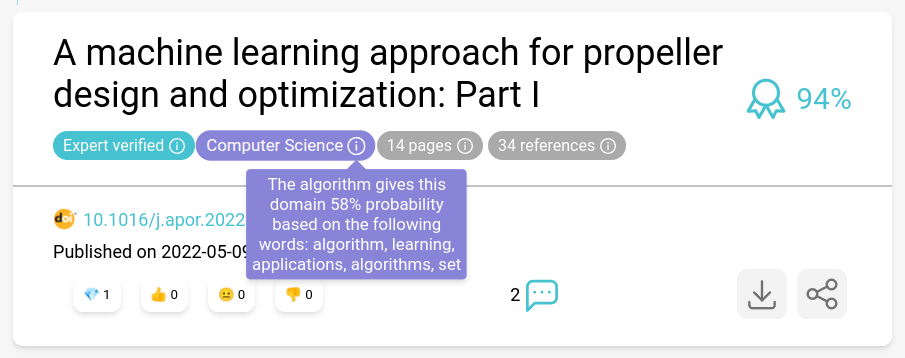
\includegraphics[width=0.7\linewidth]{figures/dashboard-domains.png}
    \captionsetup{width=.9\linewidth}
    \caption{Screenshot of the domain prediction integrated into the ScoutinScience platform, where it is used as a filtering option.}
    \label{fig:dashboard-domains}
\end{figure}

\section{Text summarisation with SciBERT} \label{section:complex-case}

Let us now turn our attention towards a more complex component. The ScoutinScience Dashboard\footnote{\href{https://dashboard.scoutinscience.com/}{dashboard.scoutinscience.com}} contains a full-page evaluation view for academic publications. On this, the known metadata, historical trends about the paper's topics, social media mentions, a PDF viewer showing the document, and other augmentation tools are displayed. One of these is the \textit{Highlights} section, which aims to summarise the paper from a technology-transfer perspective.

The current approach uses a simple heuristic based on a set of phrases selected by business developers and extended by the help of a word2vec model \cite{mikolov2013efficient}. The user feedback deemed this implementation slightly helpful but not adequate for providing an accurate overview. Thus, this is the baseline that I attempt to improve on in this section.

\begin{displayquote}
Compared with Section \ref{section:simple-case}, this time around, the toolset of \textit{GreatAI} is available at our disposal. Hopefully, this will streamline the development and --- especially --- the deployment. Given its arguably higher complexity, the experiment falls closer to industrial use-cases, and hence, can give more accurate feedback on how to further improve the API.
\end{displayquote}

\subsection{Background}

Automatic text summarisation (ATS) is also one of the earliest established tasks of text analysis and boasts numerous promising results \cite{el2021automatic}. Text summarisation is usually divided into extractive and abstractive approaches. Even though the latter can lead to more fluent summaries, it is also prone to hallucinate content that is unfaithful to the input \cite{maynez2020faithfulness}. For this reason, extractive techniques are preferred in this case.

Our problem requires generating a special type of summary: it must only concern a single aspect (tech-transfer) of the document. Aspect-based text summarisation has also seen some progress over the last decades \cite{berkovsky2008aspect,hayashi2021wikiasp} but these methods require concretely defined topics. Unfortunately, \textit{tech-transfer potential} is anything but a clear topic definition.

Numerous discussions and interviews with business developers over the last two years made it clear that there is no universally agreed on definition for it. At least, all of them agree that they know it when they see it. Additionally, most of them agree that they can confidently make a decision at the granularity of sentences. This gives rise to an obvious idea: show the experts something that they can annotate. Because the time of experts is valuable, and relevant sentences are few and far between, extra care needs to be taken to improve the ratio of positive examples in the dataset. The research of Iwatsuki Kenichi on formulaic expressions (FE) \cite{iwatsuki2020evaluation,iwatsuki2021extraction,iwatsuki2021communicative,iwatsuki2022extraction} provides a promising direction to do so. 

A formulaic expression is a phrase with zero or more ``slots'' which when filled appropriately, leads to expressing a certain intent. In the context of scientific texts, an example\footnote{Taken from the ground-truth data available at \href{https://github.com/Alab-NII/FECFevalDataset/blob/master/human_evaluation/background.tsv}{github.com/Alab-NII/FECFevalDataset}.} could be: \texttt{it was not until * that}. The asterisk can be substituted with multiple terms and the intention of this expression is (likely) to describe the \textit{History of the related topics}. Iwatsuki et al. identified a set of 39 intentions, compiled a manually labelled dataset \cite{iwatsuki2020evaluation}, and developed multiple approaches for automatically extracting and classifying formulaic expressions in large corpora \cite{iwatsuki2021communicative,iwatsuki2022extraction}.

\subsection{Methods}

In order to compile a new dataset, experts are asked to judge sentences that passed an \textit{intention check}. This pooling approach is commonly used in the field of information retrieval \cite{schutze2008introduction}. The filtering is expected to sieve out sentences that are probably not relevant from a technology-transfer perspective using Iwatsuki's formulaic expression intention labels. Subsequently, relevance judgements --- in the form of \textit{interesting} or \textit{not interesting} labels --- are gathered for these sentences. This method turns the extractive summarisation into a binary classification task for which a SciBERT model \cite{beltagy2019scibert} can be finetuned. Ultimately, the summaries are derived from sentences that are selected by the classifier trained on the experts' annotations.

We have to note two possible shortcomings of this setup: firstly, we assume the FE intentions are strongly correlated with the sought-after aspect, this may or may not be true. secondly, only the individual relevance of the sentences is considered instead of the overall relevance (utility) of the summary. Nonetheless, it is expected that stemming from the length of the documents and the sparseness of the selected sentences, that any combination of them is likely to have low redundancy.

\subsection{Results}

For the first iteration, 1500 sentences were selected for 2 experts to annotate in a binary fashion according to strict guidelines. An example is shown in Figure \ref{fig:annotator}. Afterwards, for measuring the interrater agreement, Cohen's kappa \cite{cohen1960coefficient} is calculated as shown in Equation \ref{equation:kappa}. Which turns out to be \textbf{0.4310} for the two annotators. This happens to be just above the lower end of \textit{moderate agreement}. However, we have to note that the original quality ranges are often criticised for being too relaxed \cite{mchugh2012interrater}. However, in the case of summarisation, Verberne et al. \cite{verberne2018creating} argue that reasonable end-quality can be reached even when the interrater agreement is relatively low. The ground truth is determined by taking the logical disjunction of the annotations.

\begin{figure}
    \centering
    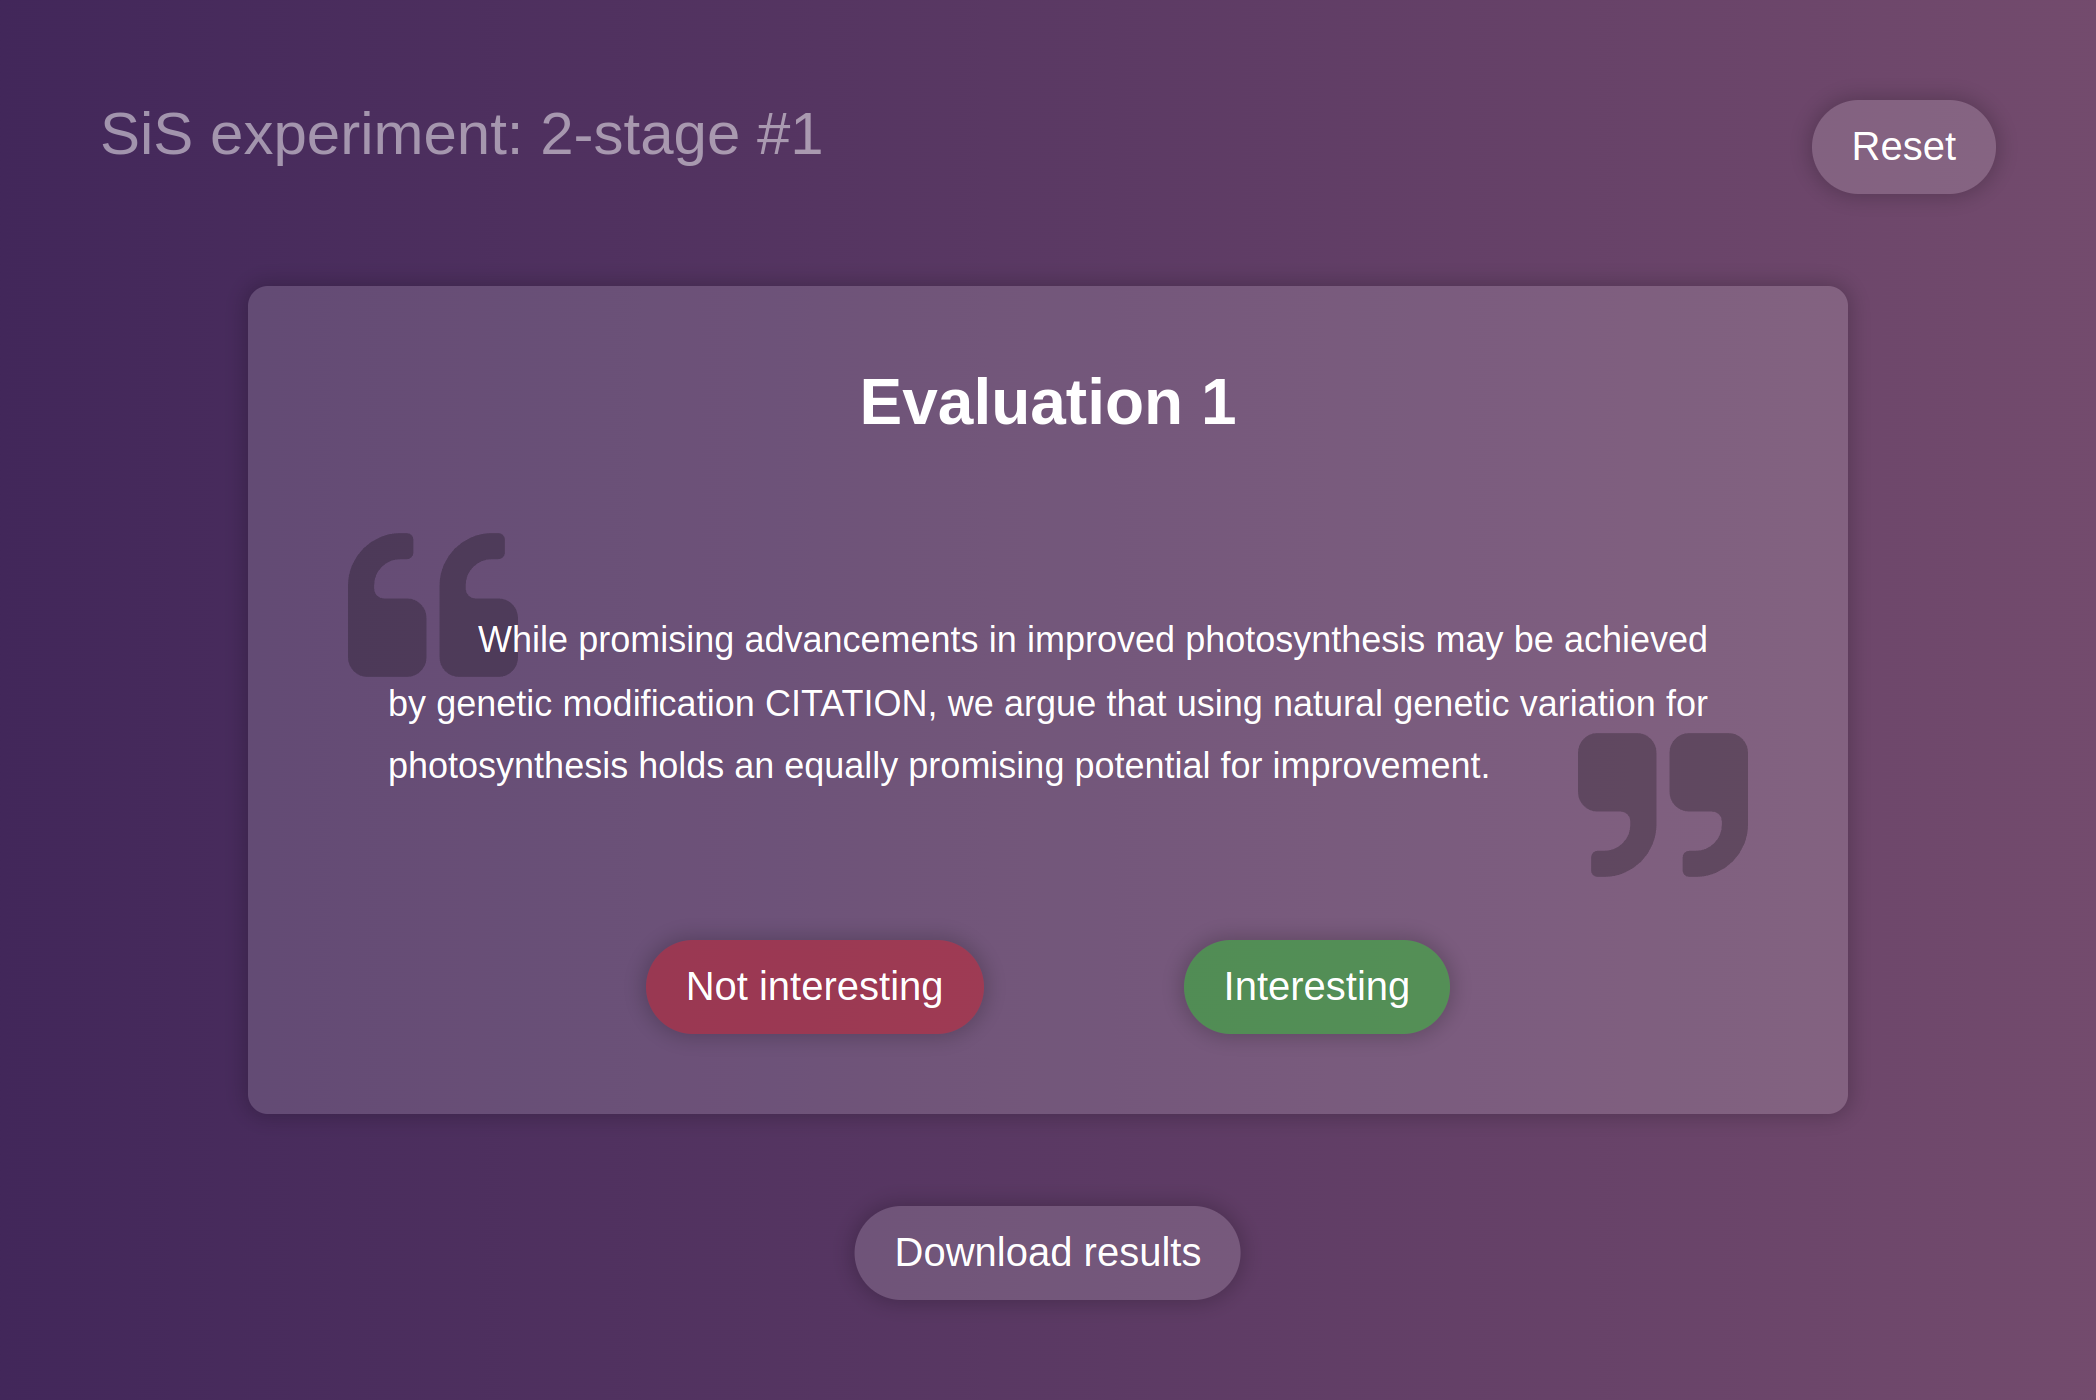
\includegraphics[width=0.75\linewidth]{figures/annotator.png}
    \captionsetup{width=.9\linewidth}
    \caption{Annotator UI showing a single sentence and the two possible labels that can be assigned to it based on its relevance to technology transfer.}
    \label{fig:annotator}
\end{figure}

\begin{equation} \label{equation:kappa}
\kappa_{agreement} \equiv \frac{p_{observed} - p_{expected}}{1 - p_{expected}} = 1 - \frac{1 - p_{observed}}{1 - p_{expected}} 
\end{equation}

The next step is finetuning SciBERT with the help of HuggingFace transformers \cite{wolf2019huggingface}. The data are divided into training and test splits with a ratio of 4:1. From the train split, a validation split is also derived which is used for early stopping. The objective function is the positive class' F1-score and the early stopping patience is 5 epochs. The learning rate is $5 \times 10^{-5}$ and AdamW \cite{loshchilov2017decoupled} is used for optimisation with a weight decay of 0.05. The code can be found in the documentation\footnote{\href{https://great-ai.scoutinscience.com/examples/scibert/train/}{great-ai.scoutinscience.com/examples/scibert/train/}}, it is surprisingly slightly shorter than the code of Section \ref{section:simple-case}.

\begin{displayquote}
\textbf{Reproducability} Reproducible experiments are generally preferred. It is easy to forget to set some seeds values and, for example, end up with different datapoints in the test-train splits during training and validation in a Continuous Integration (CI) pipeline. To facilitate reproducability, it would be useful to reset the seeds of each imported library's random number generators (RNGs) when \textit{GreatAI} is configured. Thus, a feature has been added to detect and reset RNGs of installed and imported libraries. This certainly will not solve the reproducibility crisis \cite{hutson2018artificial} on its own, however, in some cases, it can result in one fewer step to miss.
\end{displayquote}

\begin{displayquote}
\textbf{Utility of LargeFiles} For the purposes of the documentation, the finetuning was conducted in the Google Colab online environment which is excellent for providing anyone with GPU-time for free. However, notebook environments are ephemeral, resulting in the need to manually upload and download all relevant data whenever a new virtual machine (VM) instance is granted. The \texttt{LargeFile} implementation alleviated this problem by handling the uploads and downloads automatically. Of course, first, backwards compatibility had to be solved for Python 3.7 which is the only available environment in Colab.
\end{displayquote}

The best validation results were achieved after 8 epochs which was slightly more than expected but is presumably due to the weight decay. The confusion matrix on the test split can be seen in Figure \ref{fig:scibert-confusion}: regardless the subjective definition of the task, SciBERT manages to achieve good quality which is indicated by an F1-score of \textbf{0.89}.

\begin{figure}
    \centering
    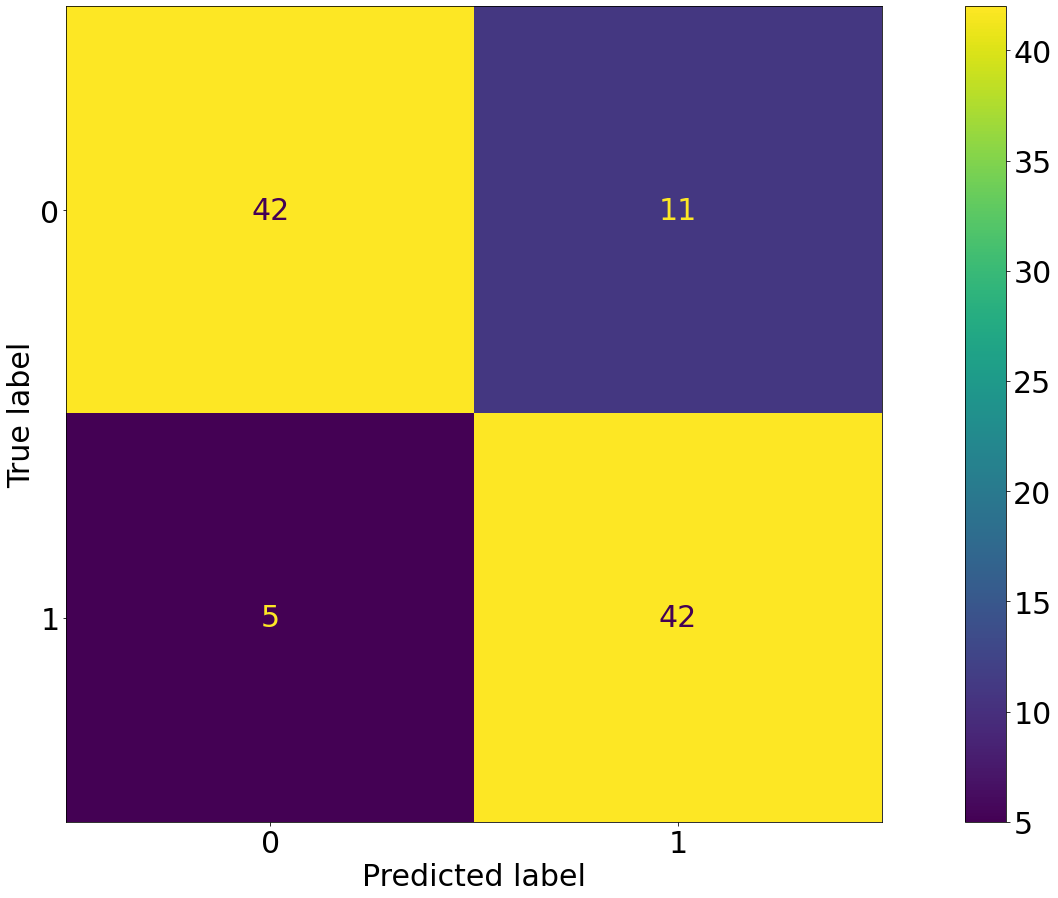
\includegraphics[width=0.4\linewidth]{figures/scibert-confusion.png}
    \captionsetup{width=.9\linewidth}
    \caption{Confusion matrix of the fine-tuned SciBERT model on the \textit{summary candidate sentences} dataset. The values are globally normalised and represent percentages.}
    \label{fig:scibert-confusion}
\end{figure}

Let us check how well the selected sentences correspond with the tech-transfer potential. Users and in-house experts can rate publications (from a tech-transfer perspective) by assigning them to one of four categories: \texttt{A}, \texttt{B}, \texttt{C}, and \texttt{D} with \texttt{A} being the most and \texttt{D} the least promising. This feedback is stored and used for analytic and training purposes. Since both the feedback grade and the ``highlights'' are supposed to reflect the same aspect of papers, therefore, we can reasonably expect some correlation between them.

Figure \ref{fig:histograms} shows the ratio of summary candidate sentences as predicted by the finetuned model in 4 categories (grades) of papers. The two datasets come from non-overlapping sets of papers, hence, the results come solely from the model's ability to generalise. It is interesting to see that the Spearman's rank correlation coefficient \cite{spearman1961proof} between the normalised ``highlights'' counts and the ratings of papers is \textbf{0.4784} and is statistically significant ($P = 5.4 \times 10^{-74}$). This proves the presence of a monotonic association. For context, the correlation between the grades and the number of sentences found by the baseline approach is 0.06597 ($P = 0.03$). We can conclude that the classifier's output is indicative of the publications' tech-transfer potential. 

\begin{figure}
    \centering
    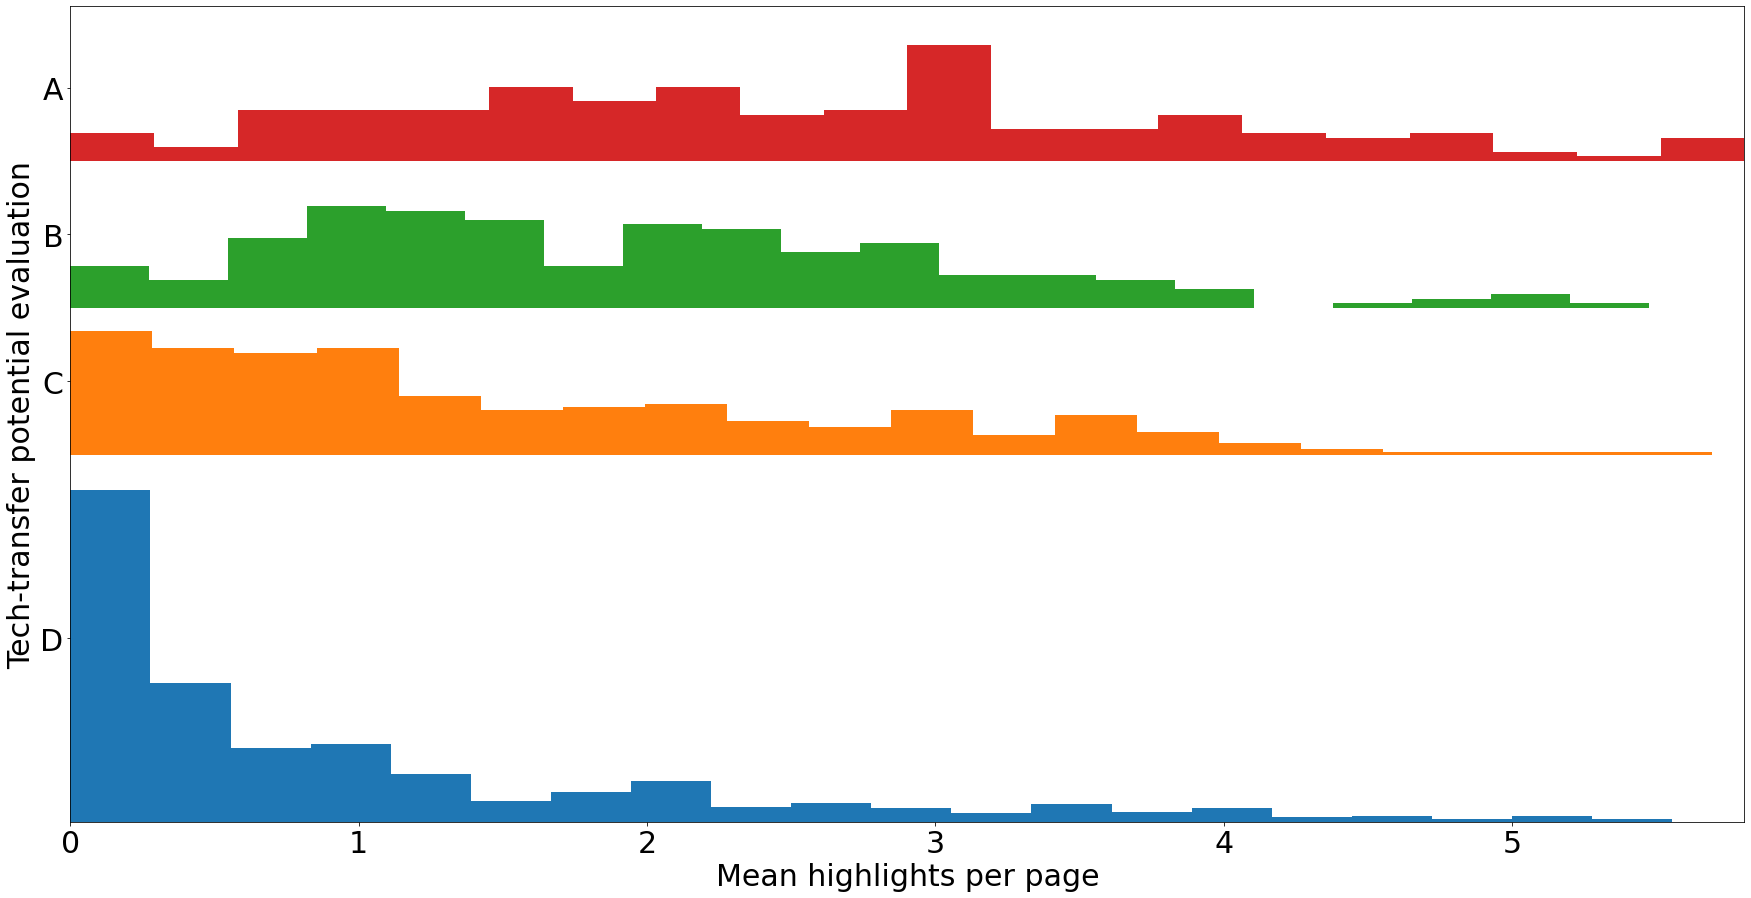
\includegraphics[width=0.85\linewidth]{figures/highlights-histograms.png}
    \captionsetup{width=.9\linewidth}
    \caption{Distribution of mean predicted summary candidate sentence counts in 4 categories. Category \texttt{A} correspond to the most, while \texttt{D} to the least interesting papers based on mean user feedback. The sample size is 1406 (\texttt{D}=715, \texttt{C}=309, \texttt{B}=198, \texttt{A}=184). The histograms are on the same scale.}
    \label{fig:histograms}
\end{figure}

\subsection{Deployment}

To implement the summarisation, at most the top 7 selected sentences are chosen as ranked by their log-probabilities. They are subsequently reordered according to their position in the text. As a quasi-explanation, the tokens' attention scores are visualised and overlaid on the highlighted sentences. The \textit{i}-th token's visualised attention comes from summing up the attention weights of each of the last layer's heads between the \texttt{[CLS]} and the \textit{i}-th token. To improve the end-user experience, a high-pass filter and a stop-word list is applied to the scores in order not to highlight the syntax-related tokens (punctuation, determiners). The service --- after being integrated into the dashboard --- can be seen in Figure \ref{fig:dashboard-highlights}.

\begin{displayquote}
In order to get insights into their inner workings, HuggingFace models can be given \texttt{output\_attentions=True} in their constructor which results in a new property becoming accessible on the results for querying the attentions. The only issue with it is that it is a 5-dimensional matrix which makes exploring and understanding it non-obvious. In short, it has very low \textit{Discoveribility}. For example, the attentions for the UI are calculated with this expression:
\begin{minted}[
baselinestretch=1,
]{python}
np.sum(result.attentions[-1].numpy()[0], axis=0)[0][1:-1]
\end{minted}
Even though the operation is conceptually simple, because of the opaque datastructure, this is anything but obvious to comprehend. Therefore, it is clear that this needs to be avoided in my library design; it has to have a clear and discoverable API which can be achieved by the use of typehints, descriptive property names, and docstrings.
\end{displayquote}

\begin{figure}
    \centering
    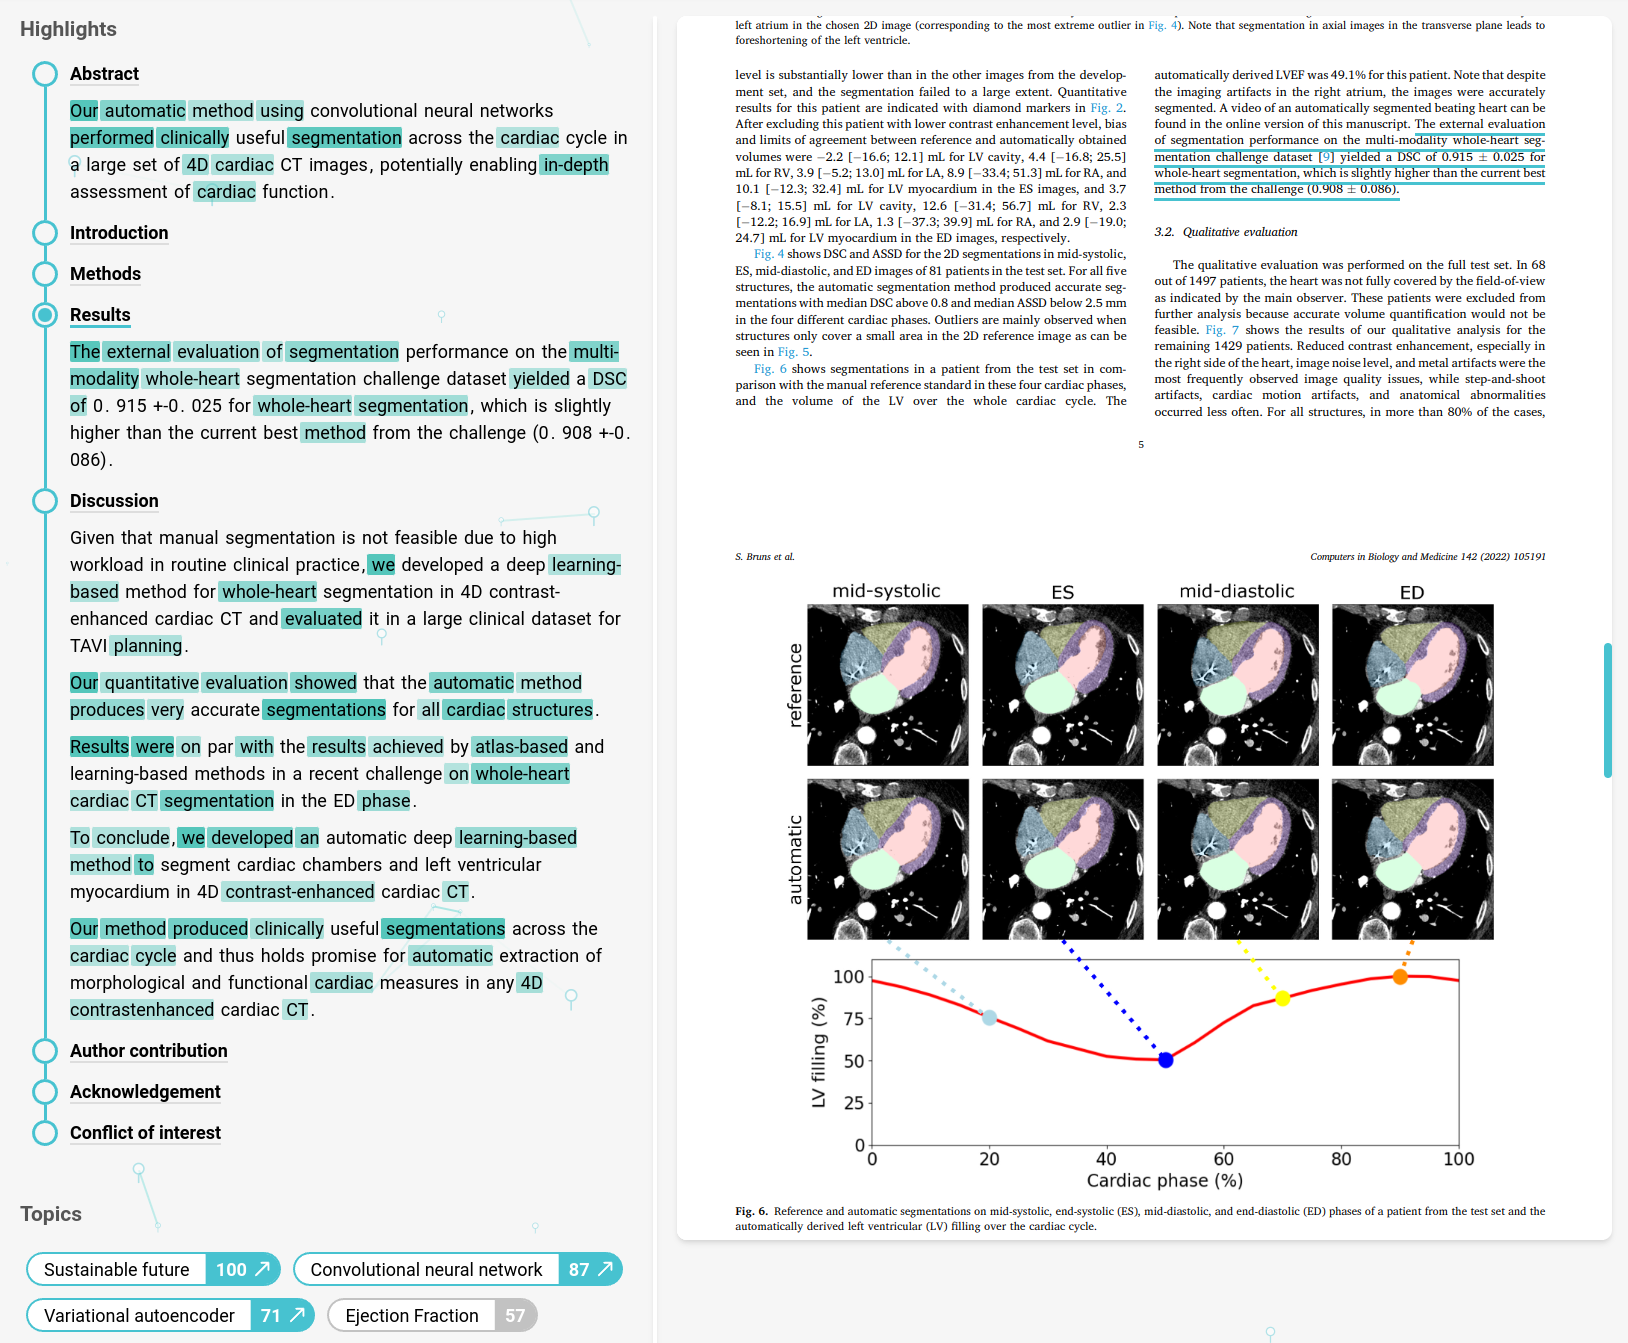
\includegraphics[width=1\linewidth]{figures/dashboard-highlights.png}
    \captionsetup{width=.9\linewidth}
    \caption{The tech-transfer summary of an academic publication (\cite{bruns2022deep}). The titles and sentences can be clicked for navigating the paper on the right, meanwhile some explanation is provided by the highlighted words, the opacity of which corresponds to their attention weights.}
    \label{fig:dashboard-highlights}
\end{figure}

\section{Improving GreatAI}

After having solved two problems by implementing two standalone services and integrating them into an existing ecosystem while relying on \textit{GreatAI} as a primary tool, a wide variety of insights have been gained. In the next couple of subsections, the extra features and design decisions are presented that have been motivated by the \textit{Highlights service}. After which, the final surface of the API is described and evaluated by its relation to the SE4ML \cite{serban2020adoption,serban2021practices} and AI engineering \cite{john2020architecting,john2020ai} best practices.

\subsection{Caching}

Sustainability is an increasingly crucial concern of ethical AI \cite{van2021sustainable}. Without discussing the pros and cons of the green computing movement \cite{10.1145/1400181.1400186}, we can still agree that computing time should not be wasted. To this end, caching the results of expensive operations has to be considered in any AI deployment. In this case, the \textit{Highlights service} is often called multiple times from different other services with the same parameters. With each operation taking up to a couple of seconds, implementing caching can lead to vastly faster response times and an overall more socially conscious deployment.

\subsection{Revisiting \texttt{parallel\_map}}

Even though most inference functions are CPU-bound, turns out, sometimes they involve IO, especially, when relying on the results of other, remote models. This means that a significant performance improvement can be achieved by implementing some inference functions asynchronously \cite{tilkov2010node}. Thus, \textit{GreatAI} also has to support decorating both regular (synchronous) and asynchronous functions. There is one notable consequence of this: the batch processing feature also has to be compatible with \texttt{async} inference functions. Batch processing is still a useful feature since it is likely that async inference functions are both IO (remote calls) and CPU (local evaluation) constrained at the same time, thus, they can benefit from multi-core parallelisation. 

However, the standard library's \texttt{multiprocessing}, the third party \texttt{multiprocess} \cite{mckerns2012building}, and, another popular library, \texttt{joblib}\footnote{\href{https://joblib.readthedocs.io/en/latest/}{joblib.readthedocs.io/en/latest}} all lack the support for efficiently parallelising async functions. For this reason, \texttt{parallel\_map} is reimplemented to create an event-loop in each worker process to keep the efficiency of non-blocking IO while also providing parallelisation for the CPU-bound sections of code.

\subsection{Programmatic integration}

Apart from supporting \texttt{async} calls, there are a couple of more step that can be taken to help integrating any service with a \textit{GreatAI} deployment. This is implemented by the \texttt{call\_remote\_great\_ai} function which hides the networking required to call a \textit{GreatAI} instance's REST API. It takes care of validation, automatic retries, serialisation, and deserialisation. This comes with the added benefit of encouraging decoupled services because the friction of integrating them is no longer noticeable which is beneficial for human collaboration \cite{hasselbring2002component}.

Additionally, a REST API is generated with its accompanying OpenAPI schema\footnote{\href{https://swagger.io/specification}{swagger.io/specification}} and served with a \href{https://swagger.io/}{Swagger} template. It also contains metadata about the function, for instance, its docstring, version, and version of its registered models concatenated in order to be SemVer\footnote{\href{https://semver.org/}{semver.org}} compatible. These can be seen in Figure \ref{fig:greatai-api}. This, combined with a \texttt{/version} HTTP endpoint for programmatic access and validation of the service's metadata proved to be key features when integrating the \textit{Highlights service} into ScoutinScience's service-based architecture.

\begin{figure}
    \centering
    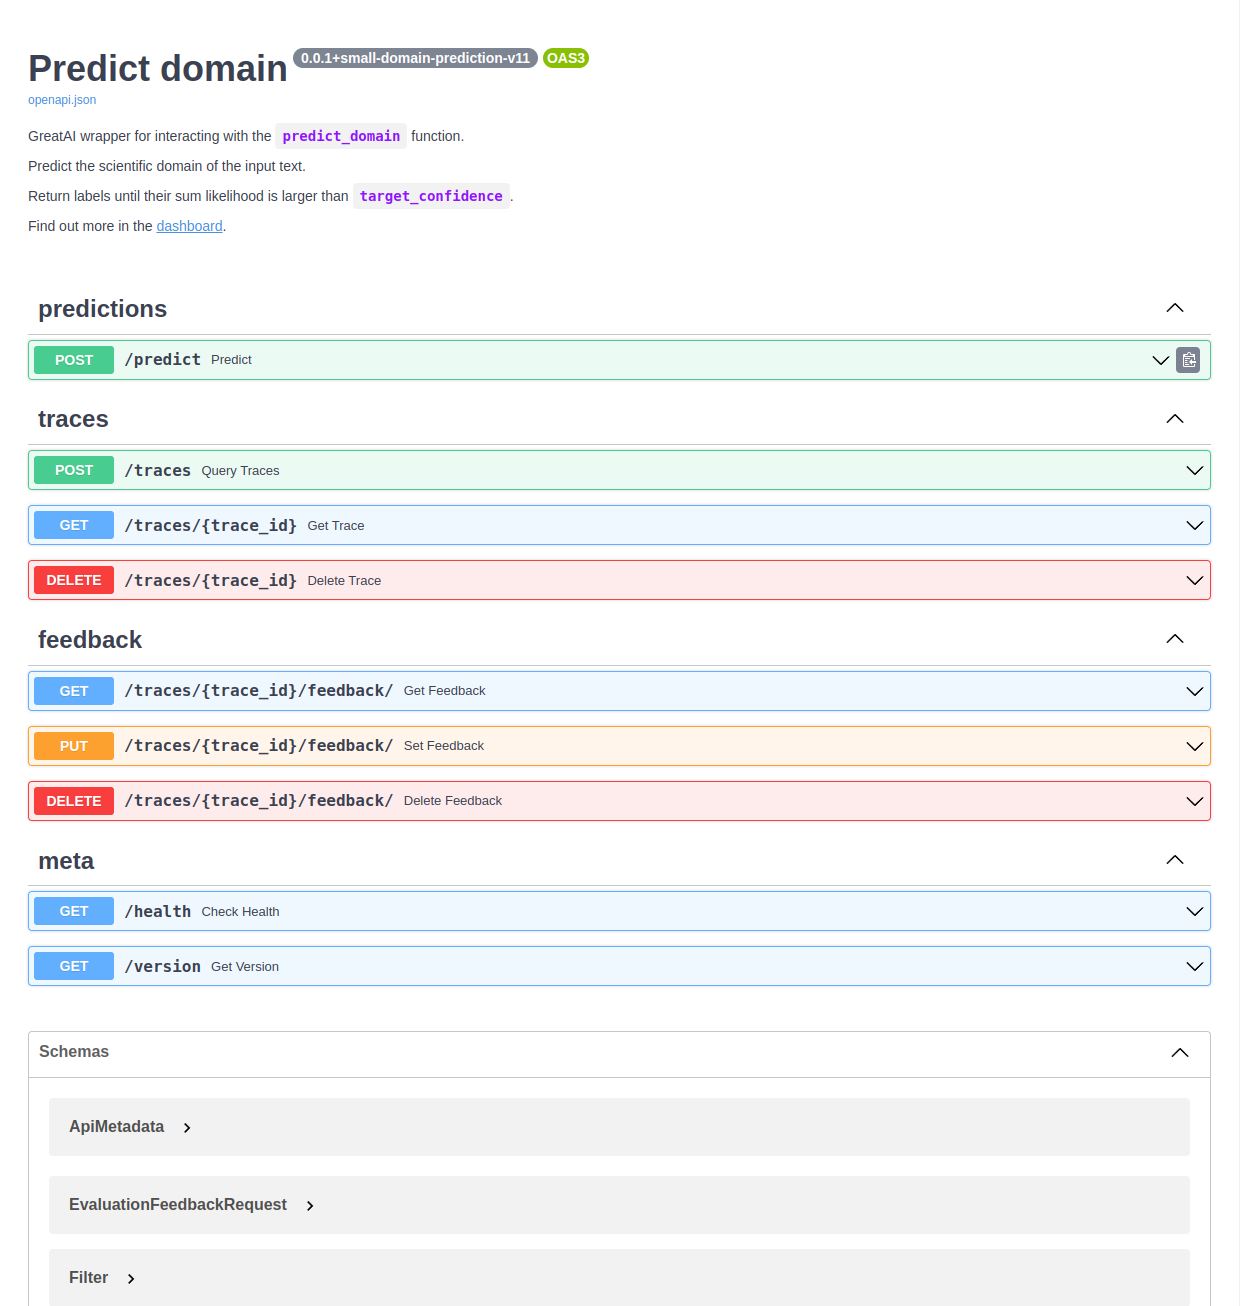
\includegraphics[width=0.85\linewidth]{figures/greatai-api.png}
    \captionsetup{width=.9\linewidth}
    \caption{Documentation of the automatically scaffolded REST API of a \textit{GreatAI} service. Notice, how its version string includes its registered models in a SemVer compliant way: \texttt{0.0.1+small-domain-prediction-v11}.}
    \label{fig:greatai-api}
\end{figure}

\subsection{\textit{Human} integration}

Even though the REST API of \textit{GreatAI} services exposes all necessary features\footnote{Such as providing feedback per prediction, complexly filtering and sorting traces, create-read-update-delete (CRUD) operations for the feedback and traces, accessing live monitoring info (current configuration, versions, cache statistics), etc.} which are great for programmatic access, these are not ideal for direct human comprehension. In order to ease the introduction of \textit{GreatAI} services, a rudimentary dashboard is --- optionally --- generated next to the REST API. The dashboard's main features can be observed in Figures \ref{fig:greatai-header}, \ref{fig:greatai-table}, and \ref{fig:greatai-parallel}. The diagrams and filterable/sortable table are interconnected and are automatically updated, the reactive behaviour is provided by the Dash framework \cite{shammamah_hossain-proc-scipy-2019}.

\begin{figure}
    \centering
    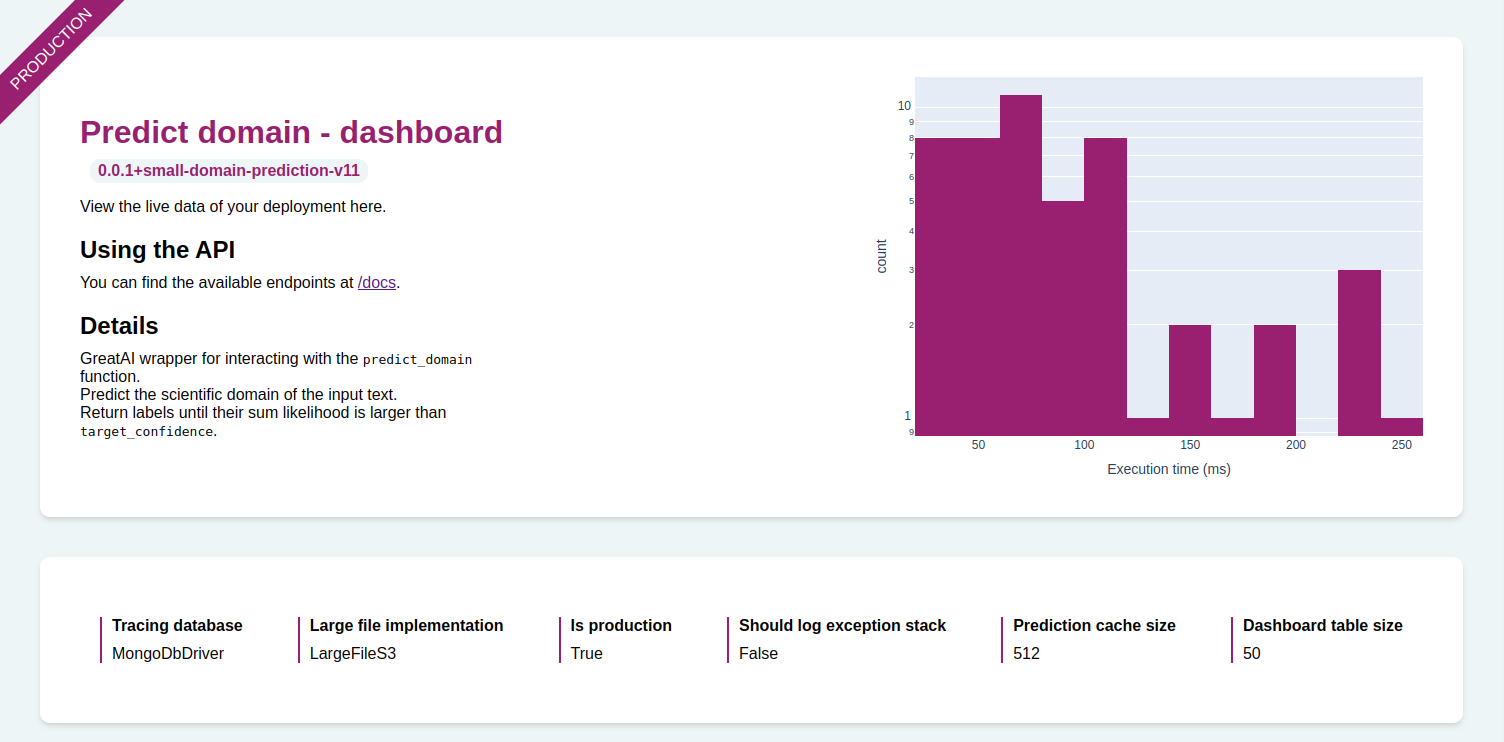
\includegraphics[width=1\linewidth]{figures/greatai-header.png}
    \captionsetup{width=.9\linewidth}
    \caption{The header of the automatically generated dashboard of the service from Section \ref{section:simple-case}. A documentation is generated on the left, while the histogram of response times is shown on the right. The current configuration is prominently displayed on the bottom.}
    \label{fig:greatai-header}
\end{figure}

\begin{figure}
    \centering
    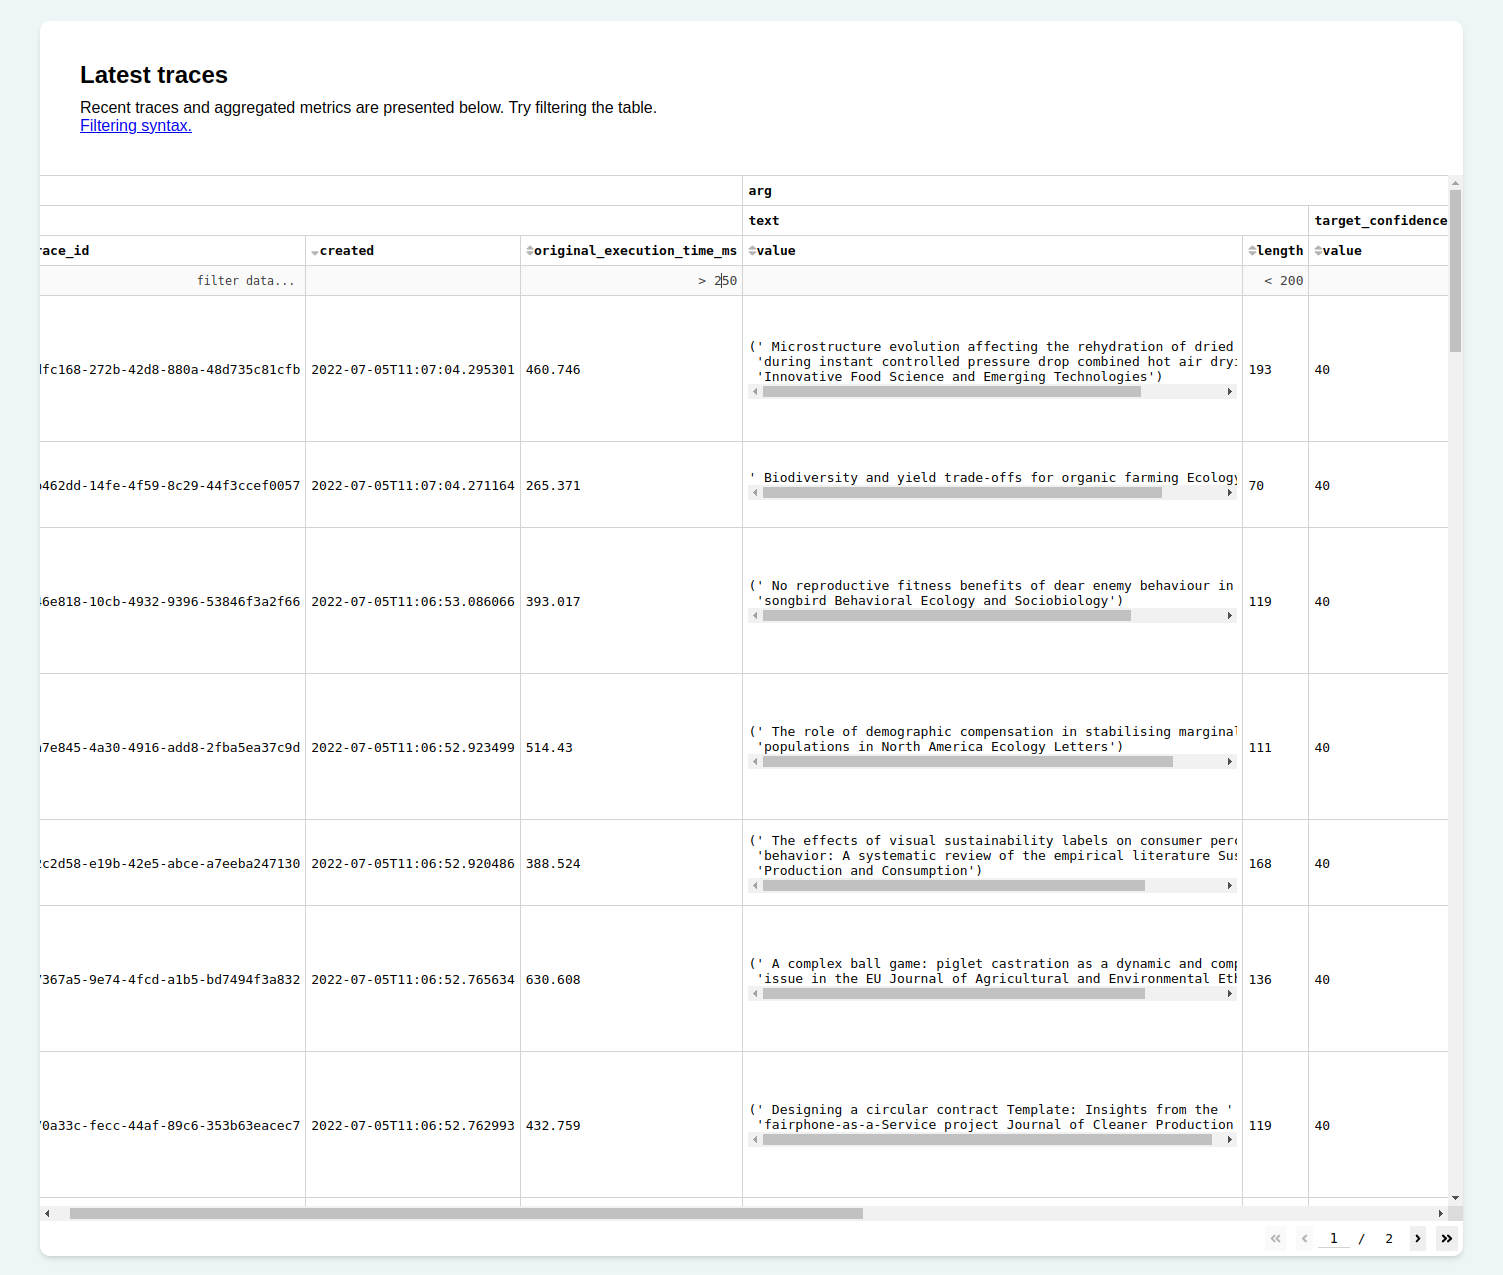
\includegraphics[width=1\textwidth]{figures/greatai-table.png}
    \captionsetup{width=.9\linewidth}
    \caption{A dynamically updating, tabular view of traces matching a user-defined filter. Useful for exploring historical predictions or debugging the cause of exceptions (which are also searchable). The filters set in the table affect the other diagrams of the dashboard.}
    \label{fig:greatai-table}
\end{figure}

\begin{figure}
    \centering
    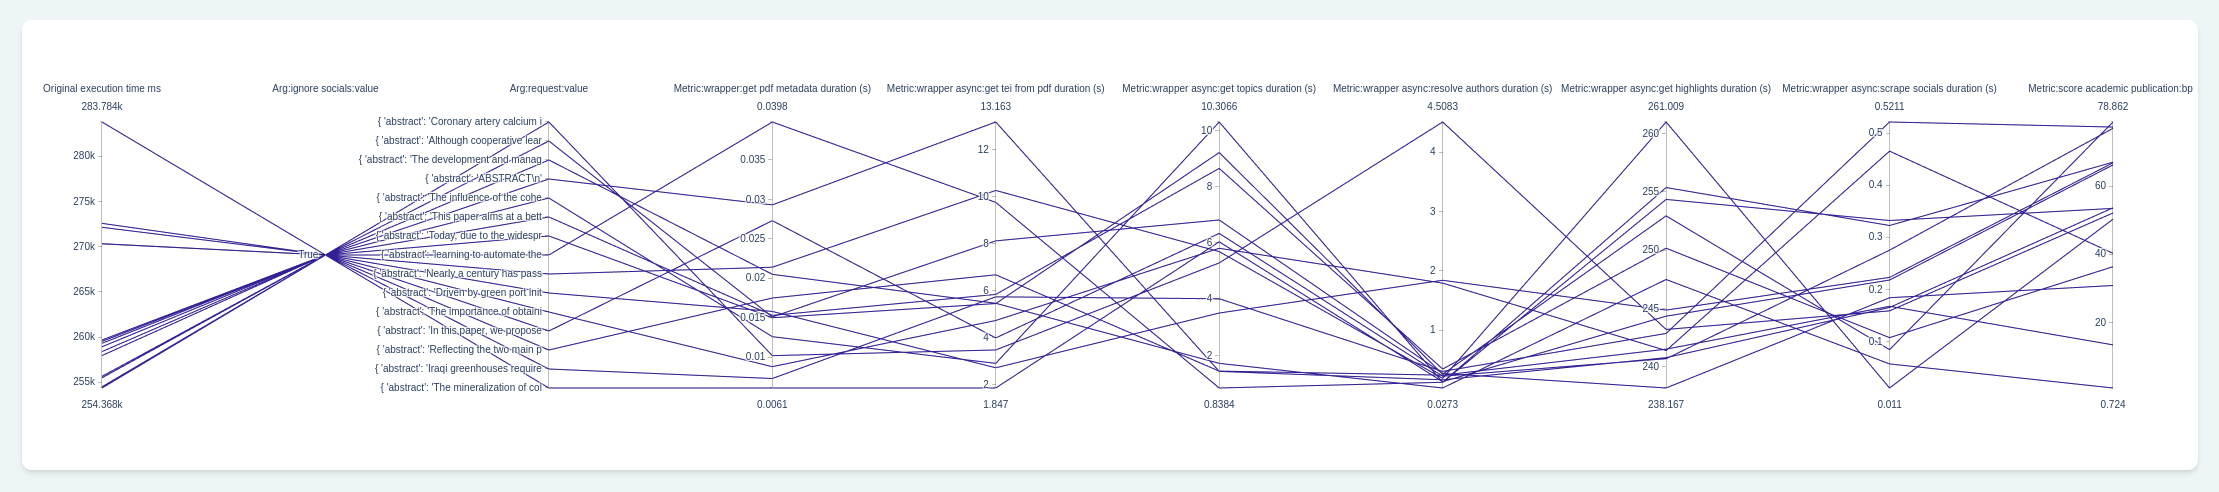
\includegraphics[width=1\textwidth]{figures/greatai-parallel.png}
    \captionsetup{width=.9\linewidth}
    \caption{A parallel coordinates view of the traces displayed in the table above. Adding new axes is as easy as calling \texttt{log\_metric} inside the inference function.}
    \label{fig:greatai-parallel}
\end{figure}


\chapter{Results \& discussion} \label{chapter:interviews}

It should not be surprising that neither data scientists nor software engineers can be replaced by software libraries. However, a non-negligible subset of their processes can be partially or fully automated, especially when it comes to packaging and deploying AI/ML services. The objective was to design a library with an API that finds the balance between being simple enough to adopt without friction yet useful enough to be adopted. Simplicity is subjective and will be discussed separately in Section \ref{section:interviews}. For now, let us look at the utility of \textit{GreatAI}.

\section{Features} \label{section:features}

For answering \textbf{RQ3} --- \textit{To what extent can \textit{GreatAI} automatically implement AI deployment best practices?} --- a comparison is presented in the following, demonstrating a subset of best practices that can be implemented/scaffolded/configured with little user input; hence, through a simple and streamlined API. Tables \ref{table:best-practices-1} and \ref{table:best-practices-2} summarise the implemented best practices in the context of methods found by prior surveys of scientific and grey literature \cite{serban2020adoption,serban2021practices,john2020architecting}.

In order to show an accurately nuanced representation, a \textit{Level of support} is determined for each best practice on a scale of \textit{Partially supported}, \textit{Supported}, and \textit{Fully automated}. For instance, \textit{Use static analysis to check code quality} from Table \ref{table:best-practices-1} is \textit{Supported} because the entire public interface of \textit{GreatAI} is correctly typed (including generics and asynchronous coroutines) and compatible with \href{https://mypy.readthedocs.io/en/stable/index.html#}{\texttt{mypy}} and \href{https://marketplace.visualstudio.com/items?itemName=ms-python.vscode-pylance}{\texttt{Pylance}}. This means that when \textit{GreatAI} is used in any Python project, various tools can be applied to statically check the soundness of the project's integration with \textit{GreatAI}. However, if the library's user does not use type hints in their code and it contains a more complex control flow, it can only be partially type-checked. In short, this best practice is supported, and a considerable part of it is already implemented by \textit{GreatAI}, but clients should still keep in mind that they might also need to make an effort to implement it fully.

This is not the case for \textit{Log production predictions with the model's version and input data} because, by default, it is automatically implemented when calling \texttt{@GreatAI.create}. Users can still specify the exact expected behaviour, e.g., where to store traces, additional metrics to log, or disabling the logging of sensitive input. Nevertheless, the best practice is already implemented reasonably well without input from the library's user.

\begin{table}
\centering
\begin{threeparttable}
\caption{A subset of AI lifecycle best practices and the level of support \textit{GreatAI} provides for them. The level of support is one of \textit{Fully automated} (\checkmark\checkmark), which means that no action is required from the user, \textit{Supported} (\checkmark) only automates the reasonably automatable aspects, while \textit{Partially supported} ($\sim$) provides some useful features, but the client is expected to build on top of these.}

\label{table:best-practices-1}
{\renewcommand{\arraystretch}{1.2} % for the vertical padding
\begin{tabular}{P{7cm}@{\hskip 0.5cm}l@{\hskip 0cm}c} \hline

\textbf{Best practice}                                                                    & \textbf{Implementation}                        & \textbf{Support}       \\\hline
Use sanity checks for all external data sources\textsuperscript{1}                        & \texttt{@parameter}                            & \checkmark             \\\hline
Check that input data is complete, balanced, and well-distributed\textsuperscript{1}      & \texttt{@parameter}                            & $\sim$                 \\\hline
Write reusable scripts for data cleaning and merging (for NLP)\textsuperscript{1}         & \texttt{utilities}                             & \checkmark\checkmark   \\\hline
Make datasets available on shared infrastructure\textsuperscript{1}                      & \texttt{large\_file}                           & \checkmark\checkmark   \\\hline
Test all feature extraction code (for NLP)\textsuperscript{1}                             & \texttt{utilities}                             & \checkmark\checkmark   \\\hline
Employ interpretable models when possible\textsuperscript{1}                              & \texttt{views}                                 & $\sim$                 \\\hline
Continuously measure model quality and performance\textsuperscript{1, 2}                  & Feedback API                                   & \checkmark             \\\hline
Use versioning for data, model, configurations and training scripts\textsuperscript{1, 2} & \texttt{@use\_model}, versioning               & \checkmark\checkmark   \\\hline
Run automated regression tests\textsuperscript{1}                                         & \texttt{*\_ground\_truth}                      & \checkmark             \\\hline
Use continuous integration\textsuperscript{1}                                             & Docker Image, WSGI application                 & \checkmark             \\\hline
Use static analysis to check code quality\textsuperscript{1}                              & Fully typed API with generics                  & \checkmark             \\\hline
Assure application security\textsuperscript{1}                                            & Code is automatically audited                  & $\sim$                 \\\hline
Automate model deployment, enable shadow deployment\textsuperscript{1, 2}                 & Docker Image \& scripts                        & \checkmark             \\\hline
Enable automatic rollbacks for production models\textsuperscript{1, 2}                    & Docker Image \& scripts                        & $\sim$                 \\\hline
Continuously monitor the behaviour of deployed models\textsuperscript{1, 2}               & Dashboard, metrics endpoints                   & \checkmark\checkmark   \\\hline
Log production predictions with the model's version and input data\textsuperscript{1}     & \texttt{@GreatAI.create}                       & \checkmark\checkmark   \\\hline

\end{tabular}}
\begin{tablenotes}
    \item[1] SE4ML best practices from Table 2 of \cite{serban2020adoption}, and Table 1 of \cite{serban2021practices}.
    \item[2] Reported state-of-the-art and state-of-practice practices from Tables 2, 3, and 4 of \cite{john2020architecting}.
\end{tablenotes}
\end{threeparttable}
\end{table}

\begin{table}
\centering
\begin{threeparttable}
\caption{A subset of AI lifecycle best practices and the level of support \textit{GreatAI} provides for them. The level of support is one of \textit{Fully automated} (\checkmark\checkmark), which means that no action is required from the user, \textit{Supported} ($\checkmark$) only automates the reasonably automatable aspects, while \textit{Partially supported} ($\sim$) provides some useful features but the client is expected to build on top of these.}

\label{table:best-practices-2}
{\renewcommand{\arraystretch}{1.2} % for the vertical padding
\begin{tabular}{P{7cm}@{\hskip 0.5cm}l@{\hskip 0cm}c} \hline

\textbf{Best practice}                                                                    & \textbf{Implementation}                        & \textbf{Support}       \\\hline
Execute validation techniques: error rates and cross-validation\textsuperscript{2}        & \texttt{*\_ground\_truth}                      & \checkmark             \\\hline
% Track models, dependencies, experiments, versions\textsuperscript{2}                    & \texttt{great\_ai.use\_model}, Dashboard       & \checkmark\checkmark   \\\hline
Store models in a single format for ease of use\textsuperscript{2}                        & \texttt{save\_model}                           & \checkmark\checkmark   \\\hline
Rewrite from data analysis to industrial development language\textsuperscript{2}          & Jupyter Notebook deployment                    & \checkmark             \\\hline
Equip with web interface, package image, provide REST API\textsuperscript{2}              & \texttt{@GreatAI.create}                       & \checkmark\checkmark   \\\hline
Provide simple API for serving batch and real-time requests\textsuperscript{2}             & \texttt{@GreatAI.create}                       & \checkmark\checkmark   \\\hline
For reproducibility, use standard runtime and configuration files\textsuperscript{2}      & \texttt{utilities.ConfigFile}, Dockerfile      & \checkmark             \\\hline
Integration with existing data infrastructure\textsuperscript{2}                          & GridFS, S3 support                             & \checkmark\checkmark   \\\hline
Select ML solution fully integrated with databases\textsuperscript{2}                     & MongoDB, PostgreSQL support                    & \checkmark\checkmark   \\\hline
Querying, visualising and understanding metrics and event logging\textsuperscript{2}      & Dashboard, Traces API                          & \checkmark\checkmark   \\\hline
% Monitor status and performance\textsuperscript{1, 2}                                    & Dashboard, Status (metadata) API               & \checkmark\checkmark   \\\hline
Measure accuracy of deployed model to ensure data drifts are noticed\textsuperscript{2}   & Feedback API                                   & \checkmark             \\\hline
Apply automation to trigger model retraining\textsuperscript{2}                           & Feedback API                                   & $\sim$                 \\\hline
% Employ Agile, DevOps-style workflows, allow automatic rollback\textsuperscript{2}       & Docker Image, WSGI application                 & \checkmark             \\\hline
% Deploy different versions of same application\textsuperscript{2}                        & Complex versioning support                     & $\sim$                 \\\hline
Allow experimentation with the inference code\textsuperscript{3}                          & Development mode \& auto-reload                & \checkmark\checkmark   \\\hline
Keep the model's API and documentation together\textsuperscript{3}                        & Dashboard and Swagger                          & \checkmark\checkmark   \\\hline
Parallelise feature extraction\textsuperscript{3}                                         & \texttt{parallel\_map}                         & \checkmark\checkmark   \\\hline
Cache predictions\textsuperscript{3}                                                      & \texttt{@GreatAI.create}                       & \checkmark\checkmark   \\\hline
Support asynchronous top-down chaining of models\textsuperscript{3}                       & All decorators support async                   & \checkmark\checkmark   \\\hline
Implement standard schemas for common prediction tasks\textsuperscript{3}                 & \texttt{views}                                 & \checkmark             \\\hline

\end{tabular}}
\begin{tablenotes}
    \item[2] Reported state-of-the-art and state-of-practice practices from Tables 2, 3, and 4 of \cite{john2020architecting}.
    \item[3] Additional software engineering best practices applicable to AI/ML deployments encountered while designing and using \textit{GreatAI}.
\end{tablenotes}
\end{threeparttable}
\end{table}

\FloatBarrier

In Table \ref{table:best-practices-2}, we added six additional best practices, which are generally well-known software engineering considerations that are also applicable to AI/ML deployments. These had not explicitly made it into the aforementioned surveys; however, according to the insights gained from Sections \ref{section:simple-case} and \ref{section:complex-case}, implementing them has a positive effect on deployment quality. In future research, attention could be given to their level of industry-wide adoption and quantitative utility.

Quantifying the number of implemented best practices would be misleading since their scope and importance cover a wide range; furthermore, there is some overlap between the different studies and even within the studies. However, it is still clear that a large number of best practices (17) can be given a \textit{Fully automated} implementation by \textit{GreatAI}'s design, and many others (16) can be augmented by the library. This proves the feasibility of designing simple APIs using the techniques of Chapter \ref{chapter:design} for decreasing the complexity of correctly deploying AI services while still implementing various best practices (\textbf{RQ2}).

\section{Interviews} \label{section:interviews}

One of the central takeaways of Section \ref{section:existing} is that, for example, Seldon Core is useful for implementing or helping to implement most of the best practices. Regardless, it also has an initial threshold that must be surmounted before implementing even a single one. According to the adoption rate surveys, this may discourage a large portion of practitioners from using it or other similar frameworks. The presented solution offers a different mix of features: the initial threshold is virtually non-existent; hence, best practices can be applied immediately. But at the same time, it only covers a more limited range of practices. 

Our hypothesis is that the latter approach aligns better with the expectations of professionals. To verify this, we conducted a series of interviews with the cooperation of ten industry practitioners with varying levels of Software Engineering (SE) and Data Science (DS) experience. In this section, the question of generalisability (\textbf{RQ4}) is investigated using the interview methodology described in Section \ref{section:interview-setup}. The participants were gathered through the recommendations of my friends and colleagues. All of the final interviewees have had at least some expertise in both DS (with a median of 2.5 years) and SE (with a median of 2 years).

\subsection{Best practices survey} \label{subsection:best-practices-survey-results}

The practitioners were first asked to fill out a questionnaire about their latest AI/ML project involving deployment. This point-in-time measurement (shown in Appendix \ref{appendix:practices}) served as a baseline for the deployment quality they are used to. Analysing the results show that the amount of software engineering experience has a moderately strong correlation ($r_{Pearson} = 0.67$ with $p = 0.0033$) with the overall number and extent of implemented deployment best practices. This is illustrated in Figure \ref{fig:adoption}. Interestingly but unsurprisingly, there is no similar statistically significant relationship regarding the amount of data science experience. 

The y-axis of Figure \ref{fig:adoption} is calculated by discarding the \textit{Not applicable} answers and projecting the 5-point Likert scale to a range from 0 to 1, which is subsequently averaged over all questions. The overall mean adoption rate/extent is just above 0.5, which equates to the \textit{Neither agree nor disagree} label. These data are in line with the findings of Serban et al. \cite{serban2020adoption}.

Because the survey's 15 questions were compiled from the \textit{Fully automated} rows of Tables \ref{table:best-practices-1} and \ref{table:best-practices-2}, that means that when using \textit{GreatAI}, they are all implemented automatically. Consequently, the adoption rate/extent is doubled immediately just by wrapping the inference function with \texttt{@GreatAI.create}: this is the added value of \textit{GreatAI}\footnote{As explained earlier, measuring quality as a function of best practice count would be dubious. Thus, the achieved magnitude of the doubling is irrelevant; however, the direction of change is not.}. Moreover, this provides further evidence for answering \textbf{RQ3} showing the extent of automatically implemented practices over non-\textit{GreatAI} deployments.

\begin{figure}
    \centering
    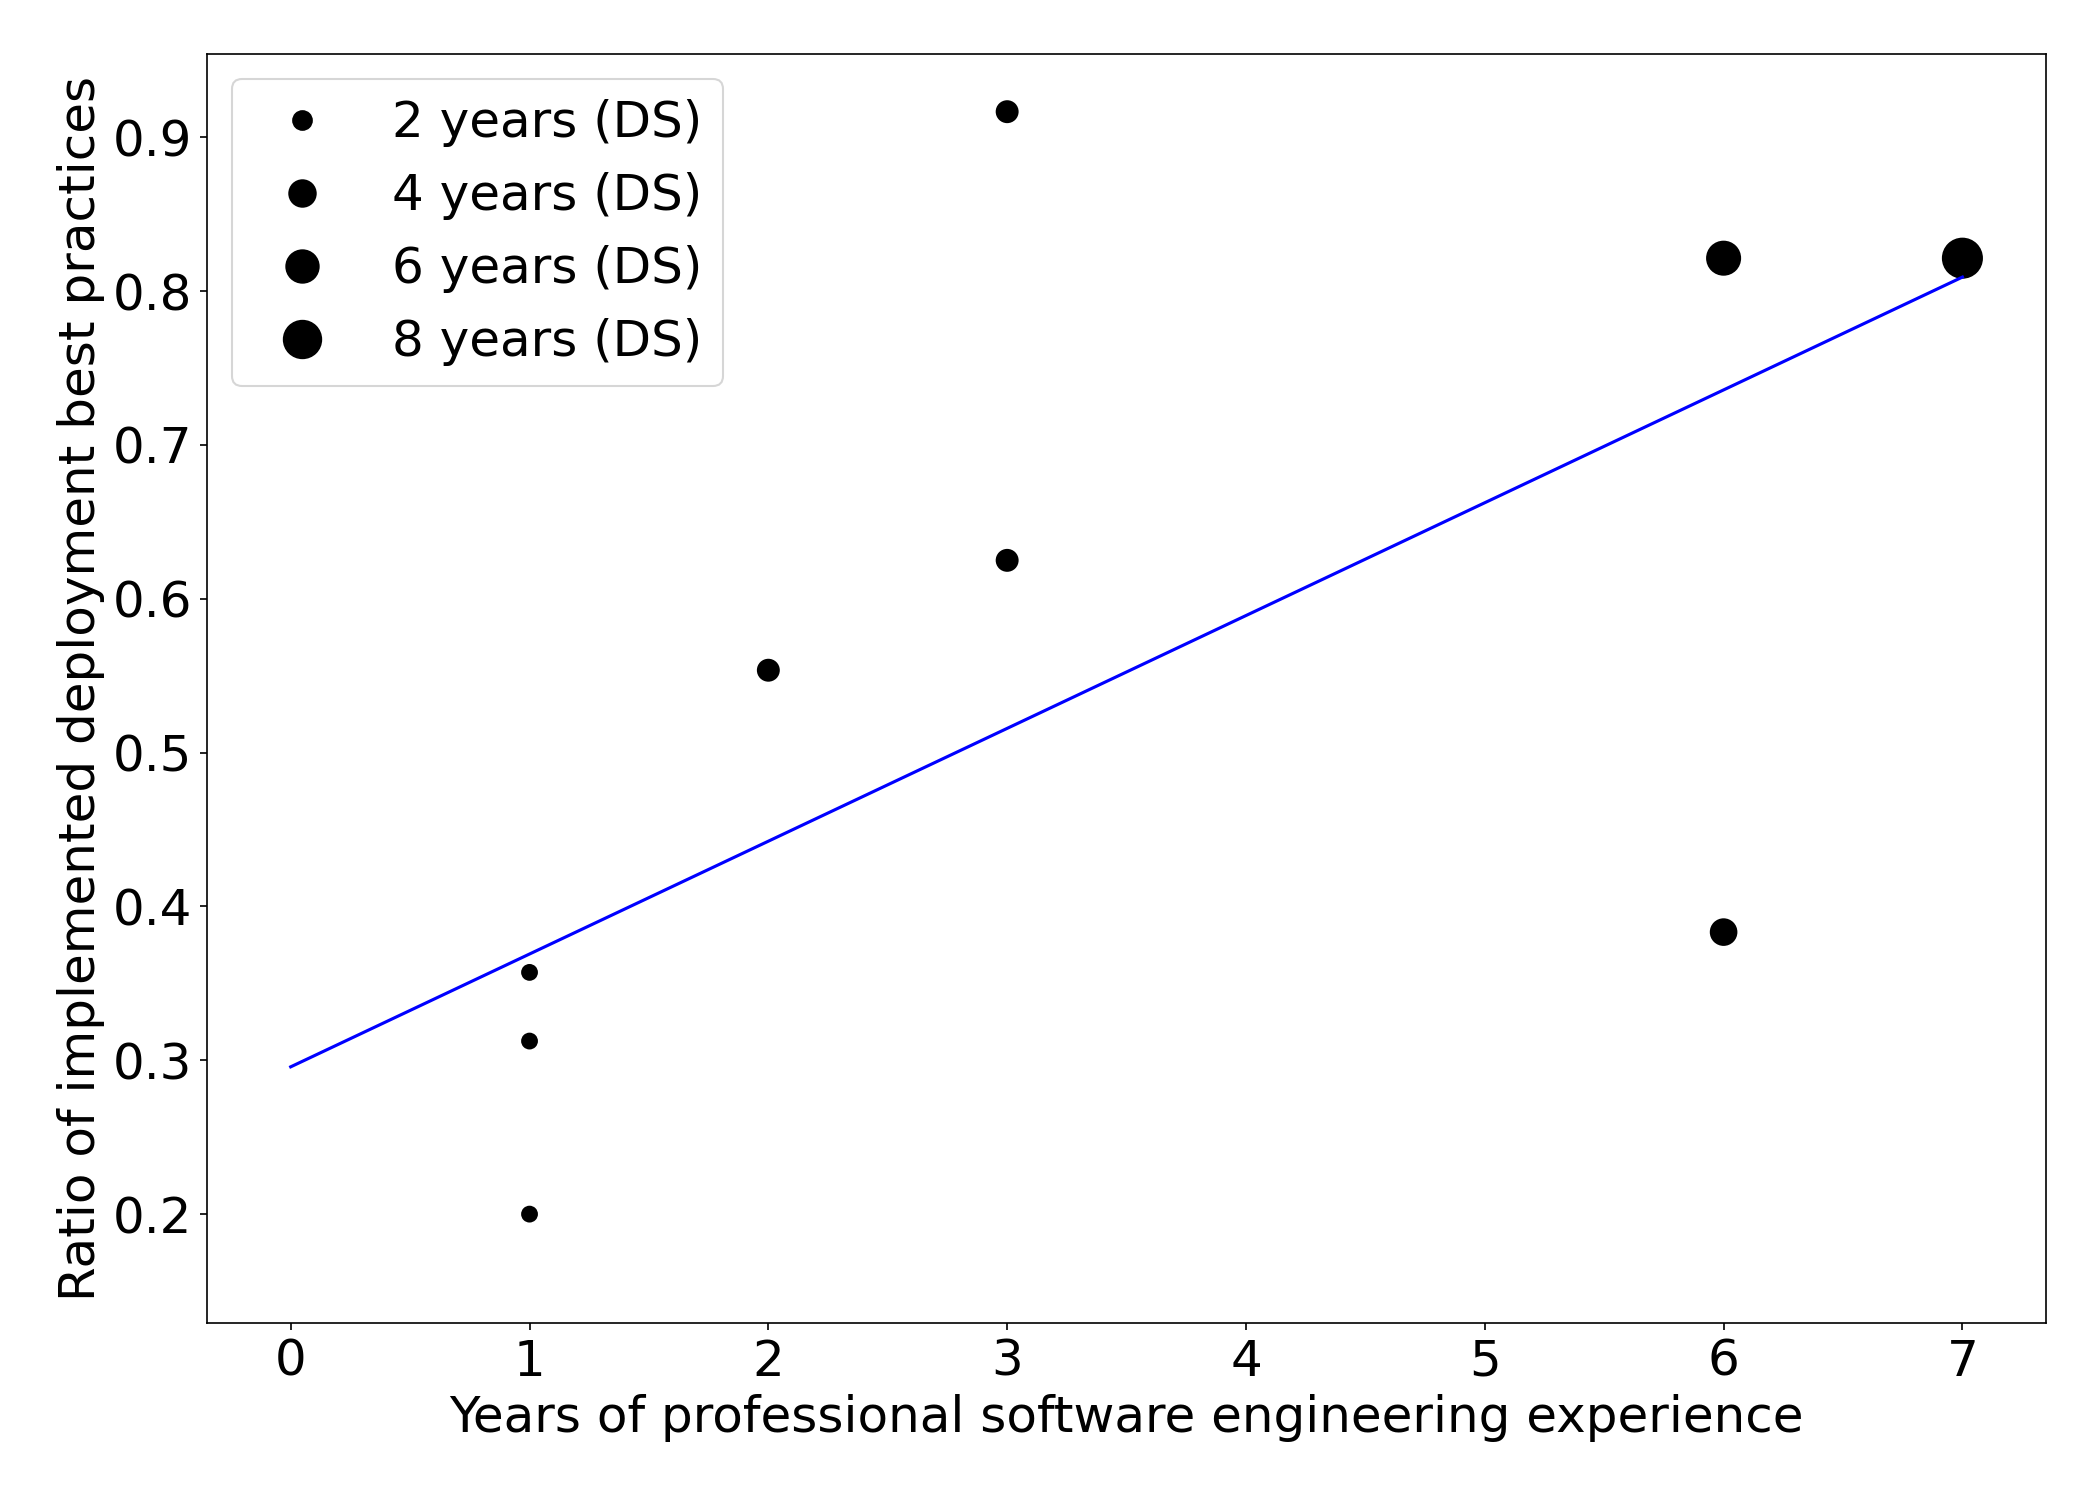
\includegraphics[width=0.6\linewidth]{figures/best-practices.png}
    \captionsetup{width=.9\linewidth}
    \caption{Best practices adoption rate as a function of Software Engineering (SE) and Data Science (DS) experience. SE experience is shown on the horizontal axis, while the point sizes denote the practitioners' experience in DS. The correlation between the axes is significant ($r_{Pearson} = 0.67$ with $p = 0.0033$).}
    \label{fig:adoption}
\end{figure}

\subsection{Technology acceptance}

\begin{table}[H]
\centering
\captionsetup{width=.9\linewidth}
\caption{Technology acceptance model survey (presented in Appendix \ref{appendix:questions}, sample size = 10) results per variable. The input values range from 1 to 7.}
\label{table:tam}
{\renewcommand{\arraystretch}{1.1} % for the vertical padding
\begin{tabular}{|r|l|l|l|} \hline
                            & \textbf{Perceived ease of use} & \textbf{Perceived utility} & \textbf{Intention to use} \\\hline
\textbf{Median}             & 5.8                          & 6.4                      & 6.3                     \\\hline
\textbf{Mean}               & 5.5                          & 6.1                      & 6.0                     \\\hline
\textbf{Standard deviation} & 1.0                          & 0.9                      & 1.3                     \\\hline
\textbf{Cronbach's alpha}   & 0.77                         & 0.88                     & 0.95                     \\\hline
\end{tabular}}
\end{table}

The participants filled out a form (shown in Appendix \ref{appendix:questions}) after finishing their first deployment with \textit{GreatAI} to provide data for creating the technology acceptance model of the problem context. The survey contained ten questions from three categories, which could be rated on a 7-point Likert scale. The summary of the answers is presented in Table \ref{table:tam}. The high Cronbach's alpha values indicate strong internal consistency \cite{nunnally1994psychometric} for each TAM dimension; thus, averaging the responses per category is semantically meaningful.

Following the methodology of \cite{cruz2019catalog}, the connections between the Perceived Utility (PU), Perceived Ease Of Use (PEOU), and Intention To Use (ITU) dimensions of TAM were analysed. Two statistically significant ($P \leq 0.05$) correlations were uncovered: between PU and ITU ($r_{Pearson} = 0.81$ with $p = 0.0048$); and PEOU and ITU ($r_{Pearson} = 0.80$ with $p = 0.0068$). Learning from the findings of prior case studies, it is reasonable to believe that both the \textit{perceived utility} and the \textit{perceived ease of use} play an equally important role in influencing professionals' \textit{intention to use} the deployment framework.

The assessment of \textit{ease of use} lags behind the rest, but it is still quite high. It may be possible that PEOU would go up with further use. Nevertheless, the high \textit{perceived utility} implies that \textit{GreatAI} shows its value early on. This, combined with the correlations uncovered within the context's technology acceptance model, validates the hypothesis that focusing on good API design is just as necessary as providing practical features.

\subsection{Task solving \& exit interviews}

In order to give qualitative depth to the previously presented quantitative results, it is time to discuss the main segment of the interviews. The participants' backgrounds covered a vast and fascinating cross-section of industrial AI/ML. The financial sector was represented by a researcher working on market prediction models for the Hungarian State Treasury and two people building an upcoming digital bank's core services. Image processing contexts were illustrated by professionals predicting Sun activity at the European Space Agency and different ones creating pose-recognition at a startup for people with disabilities using 3D cameras. Moreover, investigating companies' AI use as part of due diligence processes and intrusion detection from network packet traces are just some of the other core activities the interviewees had been doing recently. 

Stemming from this diversity, these semi-structured interviews could be expected to provide valuable insights into the generalisability of \textit{GreatAI}. The methodology of Section \ref{section:interview-setup} was followed by applying reflective journaling and thematic analysis. After labelling each aspect of the feedback, and two iterations of merging redundant or related topics, we ended up with three overarching themes: \textit{Functionality}, \textit{API}, and \textit{Responsibility to adopt}. As we will soon see, these correspond to the \textit{perceived utility}, \textit{perceived ease of use}, and \textit{intention to use} components of TAM fairly well.

\paragraph{Functionality} The library's feature-set was complimented during most interviews, with one participant noting that, although the overall number of features is relatively small, most of them are utilised in most cases. Similarly, the \texttt{utilities} submodule was appreciated for helping greatly in the interview task, but non-NLP researchers noted its likely inadequacy for their area. Still, they would like to see ``bundle'' or ``toolbox''-style modules for their fields because it would save them from a lot of copy-pasting.

The effortless parallel feature extraction and large file handling support were highlighted multiple times for the reason that the particular interviewees had not encountered other libraries providing these features. Other concrete features, such as the searchable \textit{exceptions} column in the Dashboard's table and the \textit{feedback} mechanism, were also popular. One professional highlighted the latter for coercing users to consider a human-in-the-loop approach which was said to be often expected in modern systems.

When reflecting on the framework from a bird's eye view, the generality and extensibility of the API were emphasised. As explained by a senior engineer, this is mainly because once you commit to using it, it is important not to find yourself at a dead end for a specific use case forcing you to look for a different library. However, two participants also noted that for complete generality, \texttt{MATLAB} support would be necessary. Regarding non-functional features, private hosting (especially in banking and government), open-source auditability, and good scalability (by means of an external database) were the top subjects of praise.

\paragraph{API} Regarding the surface through which clients interact with the library, the feedback is also positive but more nuanced. Many participants liked that the functions' behaviour is easy to guess from their names. The decorator syntax caused minor confusion but consulting the documentation solved the issues in all three cases. The CLI app \texttt{great-ai} was appreciated for having a close to trivial signature; the participant noted that she strives to use as few CLI commands as feasible. Surprisingly, even the practitioners with more data science background appreciated the Docker support. Nonetheless, one expert had a feature request for a configuration GUI because his colleagues are used to handling MATLAB App Designer applications.

The recurring theme of the discussions focused on the question of ``\textit{How simple is too simple?}''. The argument is that an API cannot be simpler than the domain in which it exists. More precisely, it can only be simpler at the cost of losing transparency. Let us take the example of saving models using \texttt{save\_model()}. If a project is set up correctly, it either has an initial \texttt{configure()} call to the storage provider backend, or it has an appropriately named credentials file in the project's root, for instance, \texttt{s3.ini} or \texttt{mongo.ini}. Once set up, it is trivial to use as long as we do not divert from the happy path. However, if an issue arises, such as an upgrade or migration of MongoDB, debugging the application is non-trivial for its lack of transparency.

In other words, we could say that the average (cognitive) complexity is low while the worst-case is as high --- if not higher --- than without using \texttt{save\_model()}. This proved to be somewhat controversial. However, ultimately, optimising the happy path of the AI/ML development lifecycle was deemed worthwhile by the participants in most cases. With the argument that the majority of the time spent during a project is spent on this path anyway. However, this raises the question of who exactly are the target users of \textit{GreatAI} and who will fix arising issues?

\paragraph{Responsibility to adopt} Let us first look at some insightful anecdotes that surfaced during the interviews. Especially in more research-oriented environments, production deployment pipelines can be of questionable robustness. This phenomenon was demonstrated by one account of a simple single-machine deployment pipeline: it is an interplay of \texttt{cron} jobs calling a series of shell and MATLAB scripts resembling a Rube Goldberg machine. But connecting a couple of Google Colab accounts to a GitHub repository and Weights\&Biases\footnote{\href{https://wandb.ai/site}{wandb.ai}} to implement parallel model training can also be found in the wild.

Moreover, various research companies were mentioned that for multiple years used to or still have an R\&D department consisting solely of data scientists. In one extreme case, the staff was described as more than 30 data scientists and 0 other technical employees. In such a setup, it is unreasonable to expect even professionals to have the capabilities and focus to set up the required foundation for handling all best practices. All but one interviewee verified this assumption. They also referred to their previous projects, which usually required many researchers and experts from various fields, and too often, software engineers had not been prioritised to be included.

Doing software engineering without software engineers is difficult. \textit{GreatAI} is not a viable replacement for any well-trained expert, though it is still better than nothing. During the interviews, we realised that the likely underlying reason for not employing AI engineers or software engineers as part of AI/ML projects is a lack of awareness. This was theorised by some and demonstrated by six participants who had, even though followed some, not explicitly sought out information on AI deployment best practices. Thus, raising awareness --- especially by presenting a value proposition, e.g. lower maintenance costs and better long-term quality --- might be crucial for improving AI deployments in general. Verifying this hypothesis could be a worthwhile direction for future research.

During the larger discussions, \textit{GreatAI} was deemed appropriate for raising awareness since it showcases how even a simple library is able to implement a lot of best practices. Additionally, it was noted that it could also be considered for one-person projects where --- by definition --- it is admissible to have no SE expert on the ``team''. To further help such cases, integrating a one-click Heroku\footnote{\href{https://www.heroku.com/}{heroku.com}} app deployment was also recommended to simplify the entire last portion of the lifecycle. 

\subsection{Discussion of interviews}

The overall takeaway from this is that most features were well-received, and the high mean value of \textit{perceived utility} is credible. The criticism of being NLP-centric is also justified: the initial scope of the proof-of-principle framework was limited to this domain. Nonetheless, learning the experts' opinion that they wish to have a similarly specific solution to their problem contexts is reassuring because it proves that the API is not only generalisable but is expected to be generalised. At the same time, it is crucial to admit that no one-size-fits-all solution can exist for such a diverse domain. Therefore, allowing customisability and easy extension of the system must remain central design questions.

Regarding the API's level of abstraction, we have to agree with the experts that the problem of deployment cannot be ``magically'' solved by a trivial API. However, solving deployment problems can be streamlined, at least in simpler cases. At the same time, the complex ones can be left to the professionals with relevant knowledge. This parallels the AI-libraries that have inspired \textit{GreatAI}. For instance, Hugging Face \texttt{transformers} streamlines fine-tuning and applying SOTA models, but it does not provide any facilities to help you create the next SOTA architecture because that is a vastly more complex task that most users are not expected to tackle.

In order to reach its goal of improving best practice adoption, \textit{GreatAI} can help raise awareness by presenting a verifiable value proposition, i.e. a couple of lines of code can already result in more maintainable, robust, high-quality deployments. This might prompt users or technical decision-makers to invest more in software engineering in AI/ML projects. Additionally, it can help the effectiveness of AI/software engineers by handling the grunt work of implementing some best practices, leaving them with more resources to focus on the complex and creative aspects of \textit{GREAT} deployments.
  
In summary, the answer to \textit{How suitable is the design of GreatAI for helping to apply best practices in other contexts?} (\textbf{RQ4}) is --- unsurprisingly --- subjective. Combining the high value of \textit{intention to use} from Table \ref{table:tam}, the generally positive feedback regarding the library's added value, and the numerous feature requests for fitting it to specific needs, we conclude that there is some chance of suitability for generalisability. The existence of this potential is already exciting and presents an opportunity for experimenting with building on the design of \textit{GreatAI}.

\subsection{Threats to validity}

Two potential threats to the validity of the experiments and their results are identified. Firstly, the claimed utility of the framework derived in Subsection \ref{subsection:best-practices-survey-results} does not take into account the practical significance of the implemented features and, therefore, may be subject to bias. However, the \textit{perceived utility} evaluations indicate that the participating engineers and scientists identify practical value in the features of \textit{GreatAI}. Nevertheless, in the future, we intend to extend the range of implemented best practices, which would in turn, give higher confidence about the achievable quantitative improvement through using the library.

Secondly, the survey answers and, in general, the interviewees may be subject to bias. The small sample size of practitioners can reasonably lead to some groups being over- or under-represented. The presence of selection bias is also plausible. These could be mitigated by gathering more data in future research. Coming from the exploratory nature of this analysis, many insights could be gained from the collected data. However, for confidently generalising the results, more data are needed.

\section{Future work} 

The primary purpose of the library was to serve as a proxy through which its design decisions could be tested and evaluated in their practical context. For this reason, its design aimed to be a proof-of-principle for validating hypotheses and answering research questions. After successfully doing that, it has been turned into a practical software library suitable for production-use\footnote{Available at \href{https://pypi.org/project/great-ai/}{pypi.org/project/great-ai} and \href{https://hub.docker.com/repository/docker/schmelczera/great-ai}{hub.docker.com/repository/docker/schmelczera/great-ai}.}. 
 
The library's main limitations come from its bias toward NLP deployments. This is not unreasonable given the design's exploratory nature and the context of the case studies. Nevertheless, future work must focus on introducing and balancing support for many more fields' deployments. Although \textit{GreatAI} has already proved its utility, it has also shown that generalising and extending its functionality would be worthwhile. Therefore, many potential improvements are presented below.

\subsection{More ML fields}

The cases presented in Chapter \ref{chapter:case} revolved around NLP. This, of course, heavily influenced the design process. The two most notable effects can be found in the REST API's \texttt{/predict} endpoint and some \texttt{utilities} functions. The former is streamlined to accept JSON-compatible data (which caters to textual and tabular data), while the latter gives robust feature extraction support only for textual input. However, in practice, sound, image, and video are also widely taken as input. Furthermore, with the rise of multimodal models \cite{gao2020survey}, even different combinations of them may be simultaneously taken as input.

Supporting the easy, direct upload of larger non-JSON files --- e.g. by saving them to S3 and showing a preview of them on the Dashboard's traces table --- and extending \texttt{utilities} to handle multimedia formats should be sufficient for counteracting the NLP bias. Hence, widely expanding the scope of applicability of \textit{GreatAI}. As we have seen in Section \ref{section:architecture}, the architecture is otherwise adequately general; therefore, incremental extensions can be applied.

\subsection{More best practices}

In order to greatly simplify its API, each \textit{GreatAI} Trace is a single document with a well-defined schema that clients can also extend by calling \texttt{log\_metric}. MongoDB provides a convenient (and popular) method for persisting such documents; however, if there is some existing database in the environment, storing Traces in that can be favourable. PostgreSQL \cite{momjian2001postgresql} is a popular choice, and it also features good JSON document support. Hence, introducing first-class integration for PostgreSQL could benefit some clients.

Data-intensive services can fall into three broad categories: online systems, batch processing, and stream processing (near-teal-time systems) \cite{kleppmann2017designing}. As of yet, \textit{GreatAI} only provides streamlined support for the first two. Thus, developer experience could be improved by providing simple, direct integration with popular message queues/protocols, such as \href{https://kafka.apache.org/}{Apache Kafka} \cite{kreps2011kafka}, \href{https://aws.amazon.com/sqs/}{AWS SQS} \cite{garfinkel2007evaluation}, or \href{https://www.amqp.org/}{AMQP} \cite{vinoski2006advanced}. Moreover, some metrics of \textit{GreatAI}, such as the cache statistics, versions, and derived data from traces, can already be conveniently queried from its REST API. Nevertheless, adding support for the de facto standard metric gathering tool, Prometheus\footnote{\href{https://prometheus.io/}{prometheus.io}}, could save the library's users from one more integration step.

The common theme among the opportunities mentioned above is that they could be implemented reasonably well without any user input, which aligns with the library's philosophy. Of course, the open-source nature of \textit{GreatAI} already allows anyone to provide support for a wide range of integrations. Additionally, the scope could be reasonably extended, i.e. more practices could be incorporated by including more criteria next to the \textit{GREAT} ones.

\chapter{Conclusion} \label{chapter:conclusion}

Concerned by the asymmetry between the industry's adoption of accessible AI/ML-libraries and existing solutions for their robust deployment, we investigated this phenomenon's causes and potential resolution. When looking at various recent case studies, a recurring theme was revealed: \textit{transitioning} from prototypes to production-ready AI/ML deployments is a source of adversity for small and large enterprises alike. Even though several frameworks and platforms exist for facilitating this step, surveys on the execution of best practices continue to expose the industry's shortcomings. This signals that existing libraries are underutilised, which may lead to poor deployments that underperform or develop issues that go unnoticed and might inflict societal harm.

We hypothesised that presenting a library which implements best practices and is also optimised for ease of adoption could help increase the overall quality of industrial AI/ML deployments. To test this, we designed and implemented a framework based on the principles of cognitive science and the prior art of software design. Subsequently, we tested and refined the design in an iterative process. First, we developed and deployed a model for classifying the domains of academic publications. Then, we fine-tuned and deployed a SciBERT model for generating publications' technology-transfer summaries. \textit{GreatAI} had been proven helpful; therefore, after feeding back the insights gained into its design, we turned it into an open-source library. Furthermore, \textit{GreatAI} has been successfully integrated into every production deployment of ScoutinScience since then and receives thousands of monthly downloads.

During the refinement of the framework, six previously unaddressed AI/ML deployment best practices were identified. Including these, the framework fully implements 17 best practices while it provides support for another 16. We validated the value provided by implementing or helping to implement these practices through interviews with ten industry professionals from various subfields.

The interview participants completed two questionnaires, the results of one of which indicated that using \textit{GreatAI} in an example task increased the number of implemented best practices, on average, by 49\% compared with their latest project. We also calculated the technology acceptance model of the context; a significantly strong correlation was measured between the \textit{perceived ease of use}, the \textit{perceived utility} and the \textit{intention to use} dimensions. Overall, proving that ease of use is just as important as core functionality when adopting AI deployment frameworks.

The open-ended exit interviews revealed that value can be derived from the library even in its current form and that the API's design has the opportunity to generalise to other fields of industrial AI/ML applications. However, they also highlighted that adoption issues do not necessarily come from a lack of willingness but a lack of awareness. Even if the returns achievable from good deployments are well worth the investment. Nevertheless, this value proposition needs to be conveyed and proved to data science professionals and technical decision-makers; and \textit{GreatAI} might just be the ideal candidate for doing that.

\textit{GreatAI} may have the potential to bridge the gap between data science and software engineering. Stemming from the bidirectional nature of bridges, we can look at the framework from two perspectives: for professionals closer to the field of data science, it provides an automatic scaffolding of software facilities that are required for deploying, monitoring, and iterating on their models. For software engineers, it highlights the necessary steps needed for robust and improvable deployments. At the same time, it also saves them from the menial work of manually implementing these constructs. While most importantly, it proves that increasing the adoption rate of AI/ML deployment best practices is feasible by designing narrower and deeper APIs.

Good deployments benefit all of us. Accordingly, continued research into the means of good deployments remains crucial. However, next to that --- as the presented results have shown --- better deployments can also be achieved by facilitating the \textit{transition} step of the AI lifecycle with a focus on adoptability. Having automated implementations, even if for just the straightforward best practices, leaves professionals additional time to tackle the more complex deployment challenges and fewer opportunities to miss critical steps. Overall, resulting in more general, robust, end-to-end, automated, and trustworthy AI deployments.


\bibliographystyle{splncs04}
\bibliography{ref}

\appendix

\chapter{Best practices assessment} \label{appendix:practices}

Similarly to the approach of \cite{serban2020adoption}, participants are asked about their team's level of adoption of AI/ML deployment best practices. The questions come from the entries of Tables \ref{table:best-practices-1} and \ref{table:best-practices-2} where \textit{GreatAI} was determined to provide a support level of \textit{Fully automated}.

\textbf{How well did the previous AI deployment that you collaborated on implement the following best practices?} \textit{Each statement can be rated on a 5-point Likert scale or as ``Not applicable''.}

\begin{enumerate}
\item Write reusable scripts for data cleaning and merging
\item Make datasets available on shared infrastructure
\item Use versioning for data, model, configurations and training scripts
\item Continuously monitor the behaviour of deployed models
\item Log production predictions with the model's version and input data
\item Store models in a single format for ease of use
\item Equip with a web interface, package image, provide REST API
\item Provide simple API for serving batch and real-time requests
\item Integration with existing data infrastructure
\item Querying, visualising and understanding metrics and event logging
\item Allow experimentation with the inference code
\item Keep the model and its documentation together
\item Parallelise feature extraction
\item Cache predictions
\item Allow robustly composing inference functions
\end{enumerate}

\chapter{TAM questionnaire} \label{appendix:questions}

Following the methodology for the parsimonious technology acceptance model of Wu et al. \cite{wu2011user}, each statement can be rated on a 7-point Likert scale.

\paragraph{Perceived usefulness (PU)}
\begin{enumerate}
 \item I believe the use of \textit{GreatAI} improves the quality of AI deployments.
 \item I believe the use of \textit{GreatAI} would increase my productivity.
 \item I believe the use of \textit{GreatAI} can lead to robust and trustworthy deployments.
 \item Overall, I found \textit{GreatAI} useful when working with AI.
\end{enumerate}

\paragraph{Perceived ease of use (PEOU)}
\begin{enumerate}
 \item I found the  \textit{GreatAI} easy to learn.
 \item I found it is easy to employ \textit{GreatAI} in practice.
 \item I found it is easy to integrate \textit{GreatAI} into an existing project.
 \item Overall, I found \textit{GreatAI} easy to use.
\end{enumerate}

\paragraph{Intention to use (ITU)}
\begin{enumerate}
 \item Assuming \textit{GreatAI} is applicable to my task, I predict that I will use it on a regular basis in the future.
 \item Overall, I intend to use the \textit{GreatAI} in my personal or professional projects.
\end{enumerate}



\end{document}
